\documentclass{jhps}
\usepackage{grffile}
\usepackage{amssymb}
\usepackage{mathtools}
\usepackage{booktabs}
\usepackage{multirow}
\usepackage{adjustbox}
\usepackage{footnote}
\usepackage{framed}
\usepackage{textcomp}
%\usepackage{verbatim}
\usepackage{adjustbox}
\usepackage{enumitem}
\usepackage{pmboxdraw} % to use UTF-8 inside a verbatim/listing environment
 % may use if needed
 %\usepackage{float}
 %\usepackage{array}
 %\usepackage{longtable}
 %\usepackage{comment}
 %\usepackage{pdflscape}
 %\usepackage{adjustbox}
 %\usepackage{tabularx}

\graphicspath{
{./assets/},
{./assets/fig/}
}

\begin{document}

\JHPSissue{0}   % keep 0 until the issue is assigned
\JHPSkeywords{performance analysis, monitoring, time series, job analysis}   % add 2-5 keywords

  % Author macro takes Name, Institution, Optional Link to the person, Optional Email
\JHPSauthor{Julian Kunkel}{University of Reading\\Reading, UK}{https://hps.vi4io.org/about/people/julian_kunkel}{j.m.kunkel@reading.ac.uk}
\JHPSauthor{Eugen Betke}{DKRZ\\Hamburg, Germany}{}{betke@dkrz.de}   % use empty email here

\title{A Workflow for Identifying Jobs with Similar I/O Behavior Utilizing Time Series Analysis}

  % add the section numbers to the listings/figures/tables
\counterwithin{lstlisting}{section}
\counterwithin{figure}{section}
\counterwithin{table}{section}

\maketitle


\begin{abstract}

One goal of support staff at a data center is to identify inefficient jobs and to improve their efficiency.
Therefore, a data center deploys monitoring systems that capture the behavior of the executed jobs.
While it is easy to utilize statistics to rank jobs based on the utilization of computing, storage, and network, it is tricky to find patterns in 100,000 jobs, i.e., is there a class of jobs that aren't performing well.
Similarly, when support staff investigates a specific job in detail, e.g., because it is inefficient or highly efficient, it is relevant to identify related jobs to such a blueprint.
This allows staff to understand the usage of the exhibited behavior better and to assess the optimization potential.

\medskip

In this article, our goal is to identify jobs similar to an arbitrary reference job. In particular, we describe a methodology that utilizes temporal I/O similarity to identify jobs related to the reference job.
Practically, we apply several previously developed time series algorithms and also utilize the Kolmogorov-Smirnov-Test to compare the distribution of the metrics.
A study is conducted to explore the effectiveness of the approach by investigating  related jobs for three reference jobs.
The data stem from DKRZ's supercomputer Mistral and include more than 500,000 jobs that have been executed for more than 6 months of operation. Our analysis shows that the strategy and algorithms are effective to identify similar jobs and reveal interesting patterns in the data.
It also shows the need for the community to jointly define the semantics of similarity depending on the analysis purpose.
%203 days.
\end{abstract}


\section{Introduction}

Supercomputers execute 1000s of jobs every day.
Support staff at a data center have two goals.
Firstly, they provide a service to users to enable them the convenient execution of their applications.
Secondly, they aim to improve the efficiency of all workflows -- represented as batch jobs -- in order to allow the data center to serve more workloads.

In order to optimize a single job, its behavior and resource utilization must be monitored and then assessed.
Rarely, users will liaise with staff and request a performance analysis and optimization explicitly.
Therefore, data centers deploy monitoring systems and staff must pro-actively identify candidates for optimization.
Monitoring and analysis tools such as TACC Stats \cite{evans2014comprehensive}, Grafana \cite{chan2019resource}, and XDMod \cite{simakov2018workload} provide various statistics and time-series data for job execution.

The support staff should focus on workloads for which optimization is beneficial, for instance, the analysis of a job that is executed once on 20 nodes may not be a good return of investment.
By ranking jobs based on their utilization, it is easy to find a job that exhibits extensive usage of computing, network, and I/O resources.
However, would it be beneficial to investigate this workload in detail and potentially optimize it?
For instance, a pattern that is observed in many jobs bears potential as the blueprint for optimizing one job may be applied to other jobs as well.
This is particularly true when running one application with similar inputs but also different applications may lead to similar behavior.
Knowing details about a problematic or interesting job may be transferred to similar jobs.
Therefore, it is useful for support staff (or a user) that investigates a resource-hungry job to identify similar jobs that are executed on the supercomputer.

It is non-trivial to identify jobs with similar behavior from the pool of executed jobs.
Re-executing the same job will lead to slightly different behavior, a program may be executed with different inputs or using a different configuration (e.g., number of nodes).
Job names are defined by users; while a similar name may hint to be a similar workload, finding other applications with the same I/O behavior would not be possible.

In the paper \cite{Eugen20HPS}, the authors developed several distance measures and algorithms for the clustering of jobs based on the time series and their I/O behavior.
These distance measures can be applied to jobs with different runtime and number of nodes utilized but differ in the way they define similarity.
They showed that the metrics can be used to cluster jobs, however, it remained unclear if the method can be used by data center staff to explore similar jobs effectively.
In this paper, we refine these algorithms slightly, include another algorithm, and apply them to rank jobs based on their temporal similarity to a reference job.

We start by introducing related work in \Cref{sec:relwork}.
In \Cref{sec:methodology}, we describe briefly the data reduction and the algorithms for similarity analysis.
We also utilize the Kolmogorov-Smirnov-Test to illustrate the benefits and drawbacks of the different methods.
Then, we perform our study by applying the methodology to three reference jobs with different behavior, therewith, assessing the effectiveness of the approach to identify similar jobs.
In \Cref{sec:evaluation}, the reference jobs are introduced and quantitative analysis of the job pool is made based on job similarity.
In \Cref{sec:timelines}, the 100 most similar jobs are investigated in more detail, and selected timelines are presented.
The paper is concluded in \Cref{sec:summary}.

\section{Related Work}
\label{sec:relwork}

Related work can be classified into distance measures, analysis of HPC application performance, inter-comparison of jobs in HPC, and I/O-specific tools.

%% DISTANCE MEASURES
The ranking of similar jobs performed in this article is related to clustering strategies.
Levenshtein (Edit) distance is a widely used distance metric indicating the number of edits needed to convert one string to another \cite{navarro2001guided}.
The comparison of the time series using various metrics has been extensively investigated.
In \cite{khotanlou2018empirical}, an empirical comparison of distance measures for the clustering of multivariate time series is performed.
14 similarity measures are applied to 23 data sets.
It shows that no similarity measure produces statistically significant better results than another.
However, the Swale scoring model \cite{morse2007efficient} produced the most disjoint clusters.
%In this model, gaps imply a cost.

% Lock-Step Measures and Elastic Measures

% Analysis of HPC application performance
The performance of applications can be analyzed using one of many tracing tools such as Vampir \cite{weber2017visual} that record the behavior of an application explicitly or implicitly by collecting information about the resource usage with a monitoring system.
Monitoring systems that record statistics about hardware usage are widely deployed in data centers to record system utilization by applications.
There are various tools for analyzing the I/O behavior of an application \cite{TFAPIKBBCF19}.

% time series analysis for inter-comparison of processes or jobs in HPC
For Vampir, a popular tool for trace file analysis, in \cite{weber2017visual} the Comparison View is introduced that allows them to manually compare traces of application runs, e.g., to compare optimized with original code.
Vampir generally supports the clustering of process timelines of a single job, allowing to focus on relevant code sections and processes when investigating many processes.

Chameleon \cite{bahmani2018chameleon} extends ScalaTrace for recording MPI traces but reduces the overhead by clustering processes and collecting information from one representative of each cluster.
For the clustering, a signature is created for each process that includes the call-graph.
In \cite{halawa2020unsupervised}, 11 performance metrics including CPU and network are utilized for agglomerative clustering of jobs showing the general effectiveness of the approach.

In \cite{rodrigo2018towards}, a characterization of the NERSC workload is performed based on job scheduler information (profiles).
Profiles that include the MPI activities have shown effective to identify the code that is executed \cite{demasi2013identifying}.
Many approaches for clustering applications operate on profiles for compute, network, and I/O \cite{emeras2015evalix,liu2020characterization,bang2020hpc}.
For example, Evalix \cite{emeras2015evalix} monitors system statistics (from proc) in 1-minute intervals but for the analysis, they are converted to a profile removing the time dimension, i.e., compute the average CPU, memory, and I/O over the job runtime.

% I/O-specific tools
PAS2P \cite{mendez2012new} extracts the I/O patterns from application traces and then allows users to manually compare them.
In \cite{white2018automatic}, a heuristic classifier is developed that analyzes the I/O read/write throughput time series to extract the periodicity of the jobs -- similar to Fourier analysis.
The LASSi tool \cite{AOPIUOTUNS19} periodically monitors Lustre I/O statistics and computes a "risk" factor to identify I/O patterns that stress the file system.
In contrast to existing work, our approach allows a user to identify similar activities based on the temporal I/O behavior recorded by a data center-wide deployed monitoring system.


\section{Methodology}
\label{sec:methodology}

The purpose of the methodology is to allow users and support staff to explore all executed jobs on a supercomputer in order of their similarity to the reference job.
Therefore, we first need to define how a job's data is represented, then describe the algorithms used to compute the similarity, and, the methodology to investigate jobs.

\subsection{Job Data}
On the Mistral supercomputer at DKRZ, the monitoring system \cite{betke20} gathers in ten seconds intervals on all nodes nine I/O metrics for the two Lustre file systems together with general job metadata from the SLURM workload manager.
The results are 4D data (time, nodes, metrics, file system) per job.
The distance measures should handle jobs of different lengths and node count.
In the open access article \cite{Eugen20HPS}\footnote{\url{https://zenodo.org/record/4478960/files/jhps-incubator-06-temporal-29-jan.pdf}}, we discussed a variety of options from 1D job-profiles to data reductions to compare time series data and the general workflow and pre-processing in detail. 
We will be using this representation.
In a nutshell, for each job executed on Mistral, they partitioned it into 10 minutes segments\footnote{We found in preliminary experiments that 10 minutes provide sufficient resolution while it reduces noise, i.e., the variation of the statistics when re-running the same job.} and compute the arithmetic mean of each metric, categorize the value into NonIO (0), HighIO (1), and CriticalIO (4) for values below 99-percentile, up to 99.9-percentile, and above, respectively. 
The values are chosen to be 0, 1, and 4 because we arithmetically derive metrics: naturally the value of 0 will indicate that no I/O issue appears; we weight critical I/O to be 4x as important as high I/O.
This strategy ensures that the same approach can be applied to other HPC systems regardless of the actual distribution of these statistics on that data center.
After the mean value across nodes is computed for a segment, the resulting numeric value is encoded either using binary (I/O activity on the segment: yes/no) or hexadecimal representation (quantizing the numerical performance value into 0-15) which is then ready for similarity analysis.
By pre-filtering jobs with no I/O activity -- their sum across all dimensions and time series is equal to zero, the dataset is reduced from 1 million jobs to about 580k jobs.

\paragraph{Binary coding}
Binary coding is a data reduction technique that represents monitoring data as a sequence of numbers, where each number stands for a specific I/O behavior.
It is applied on the hypercube, produced by the previous pre-processing steps (segmentation and categorization).
This hypercube has four dimensions (nodes, metrics, file systems and time) and is filled with categories.
The data is reduced in two steps.
First, reduction of two dimensions (nodes and file systems) and aggregation by the sum() function creates a new two-dimensional data structure (metrics and time) filled with integer values.
Second, reduction of a dimension (metrics) and mapping of integer values to a unique number (behavior mapping) creates a one dimensional data structure (time) filled with I/O behavior.
Behavior mapping is a function that maps 9 metrics to 9-bit numbers where each bit represents activity of a metric.
If the value of a metric is LowIO then the bit is set to 0 (compute intense state), else (for values HighIO and CriticalIO) it is set to 1 (IO intense state).
The following example shows a 15 segment long binary coding:

\begin{lstlisting}
jobA (after coding): [1:5:0:0:0:0:0:0:96:96:96:96:96:96:96], 'length':15
\end{lstlisting}

\paragraph{Hexadecimal coding}
Hexadecimal coding is a data reduction technique, that can be applied to the hypercube to obtain further data reduction.
After the first two pre-processing steps (segmentation and categorization), a four dimensional hypercube (nodes, metrics, file systems and time) stores performance categories.
Hexadecimal coding operates in two steps.
First, it aggregates two dimensions (nodes and file systems) by the mean() function.
What remains are two dimensions (metrics and time) and the mean values between 0 an 4.
Second, the mean values are quantized to 16 levels -- 0 = [0,0.25), 1 = [0.25,0.5), $ \ldots $ , F = [3.75, 4].
The following example shows a five segment long hexadecimal coding:

\begin{lstlisting}
jobB: 'length': 6, 'coding':
  'metric_read'	: [0:2:2:2:9],
  'metric_write'   : [0:0:0:0:0],
  ...,
  'metric_md_other': [0:0:0:F:F]
\end{lstlisting}

\subsection{Algorithms for Computing Similarity}
We reuse the B and Q algorithms developed in~\cite{Eugen20HPS}: B-all, B-aggz(eros), Q-native, Q-lev, and Q-phases.
They differ in the way data similarity is defined; either the time series is encoded in binary or hexadecimal quantization, the distance measure is the Euclidean distance or the Levenshtein-distance.
B-all determines similarity between binary codings by means of Levenshtein distance.
B-aggz is similar to B-all, but computes similarity on binary codings where subsequent segments of zero activities are replaced by just one zero.
Q-lev determines similarity between quantized codings by using Levenshtein distance.
Q-native uses a performance-aware similarity function, i.e., the distance between two jobs for a metric is $\frac{|m_{job1} - m_{job2}|}{16}$.
There are various options for how a longer job is embedded in a shorter job, for example, a larger input file may stretch the length of the I/O and compute phases; another option can be that more (model) time is simulated. In this article, we consider these different behavioral patterns and attempt to identify situations where the I/O pattern of a long job is contained in a shorter job. Therefore, for jobs with different lengths, a sliding-windows approach is applied which finds the location for the shorter job in the long job with the highest similarity.
Q-phases extract phase information and performs a phase-aware and performance-aware similarity computation.
The Q-phases algorithm extracts I/O phases from our 10-minute segments and computes the similarity between the most similar I/O phases of both jobs.
In this paper, we add a similarity definition based on Kolmogorov-Smirnov-Test that compares the probability distribution of the observed values which we describe in the following.

\paragraph{Kolmogorov-Smirnov (KS) algorithm.}
% Summary
For the analysis, we perform two preparation steps.
Dimension reduction by computing means across the two file systems and by concatenating the time series data of the individual nodes (instead of averaging them).
This reduces the four-dimensional dataset to two dimensions (time, metrics).
% Aggregation
The reduction of the file system dimension by the mean function ensures the time series values stay in the range between 0 and 4, independently of how many file systems are present on an HPC system.
Unlike the previous similarity definitions, the concatenation of time series on the node dimension preserves the individual I/O information of all nodes while it still allows comparison of jobs with a different number of nodes.
%No aggregation is performed on the metric dimension.

% Filtering
%Zero-jobs are jobs with no sign of significant I/O load and are of little interest in the analysis.
%Their sum across all dimensions and time series is equal to zero.
%Furthermore, we filter those jobs whose time series have less than 8 values.

% Similarity
For the analysis we use the kolmogorov-smirnov-test 1.1.0 Rust library from the official Rust Package Registry ``cargo.io''.
The similarity function calculates the mean inverse of reject probability $p_{\text{reject}}$ computed with the ks-test across all metrics $M$: $sim = \frac{\sum_m 1 - p_{\text{reject}(m)}}{|M|}$.

%\begin{equation}\label{eq:ks_similarity}




\subsection{Methodology}
Our strategy for localizing similar jobs works as follows:
\begin{itemize}
  \item A user\footnote{This can be support staff or a data center user that was executing the job.} provides a reference job ID and selects a similarity algorithm.
  \item The system iterates over all jobs of the job pool computing the similarity to the reference job using the specified algorithm.
  \item It sorts the jobs based on the similarity to the reference job.
  \item It visualizes the cumulative job similarity allowing the user to understand how job similarity is distributed.
  \item The user starts the inspection by looking at the most similar jobs first.
\end{itemize}
The user can decide about the criterion when to stop inspecting jobs; based on the similarity, the number of investigated jobs, or the distribution of the job similarity.
For the latter, it is interesting to investigate clusters of similar jobs, e.g., if there are many jobs between 80-90\% similarity but few between 70-80\%.

For the inspection of the jobs, a user may explore the job metadata, searching for similarities, and explore the time series of a job's I/O metrics.

\section{Reference Jobs}%
\label{sec:refjobs}

For this study, we chose several reference jobs with different compute and I/O characteristics:
\begin{itemize}
	\item Job-S: performs post-processing on a single node. This is a typical process in climate science where data products are reformatted and annotated with metadata to a standard representation (so-called CMORization). The post-processing is I/O intensive.
  \item Job-M: a typical MPI parallel 8-hour compute job on 128 nodes which write time series data after some spin up.   %CHE.ws12
	\item Job-L: a 66-hour 20-node job.
  The initialization data is read at the beginning.
  Then only a single master node writes constantly a small volume of data; in fact, the generated data is too small to be categorized as I/O relevant.
\end{itemize}

The segmented timelines of the jobs are visualized in \Cref{fig:refJobs} -- remember that the mean value is computed across all nodes on which the job ran.
This coding is also used for the Q algorithms, thus this representation is what the algorithms will analyze; B algorithms merge all timelines together as described in~\cite{Eugen20HPS}.
The figures show the values of active metrics ($\neq 0$); if few are active, then they are shown in one timeline, otherwise, they are rendered individually to provide a better overview.
For example, we can see in \Cref{fig:job-S}, that several metrics increase in Segment\,6. 
We can also see an interesting result of our categorized coding, the write bytes are bigger than 0 while write calls are 0\footnote{The reason is that a few write calls transfer many bytes; less than our 90\%-quantile, therefore, write calls will be set to 0.}.
\Cref{fig:refJobsHist} summarizes hexadecimal codings of Job-S and Job-M to histograms:
A specific histogram contains the metric of each node at every timestep -- without being averaged across the nodes.
Essentially, this data is used to compare jobs using Kolmogorov-Smirnov-Test.
The metrics at Job-L are not shown as they have only a handful of instances where the value is not 0, except for write\_bytes: the first process is writing out at a low rate.
In \Cref{fig:job-L}, the mean value is mostly rounded down to 0 except for the first segment as primarily Rank\,0 is doing I/O.

\begin{figure}
\begin{subfigure}{0.8\textwidth}
\centering
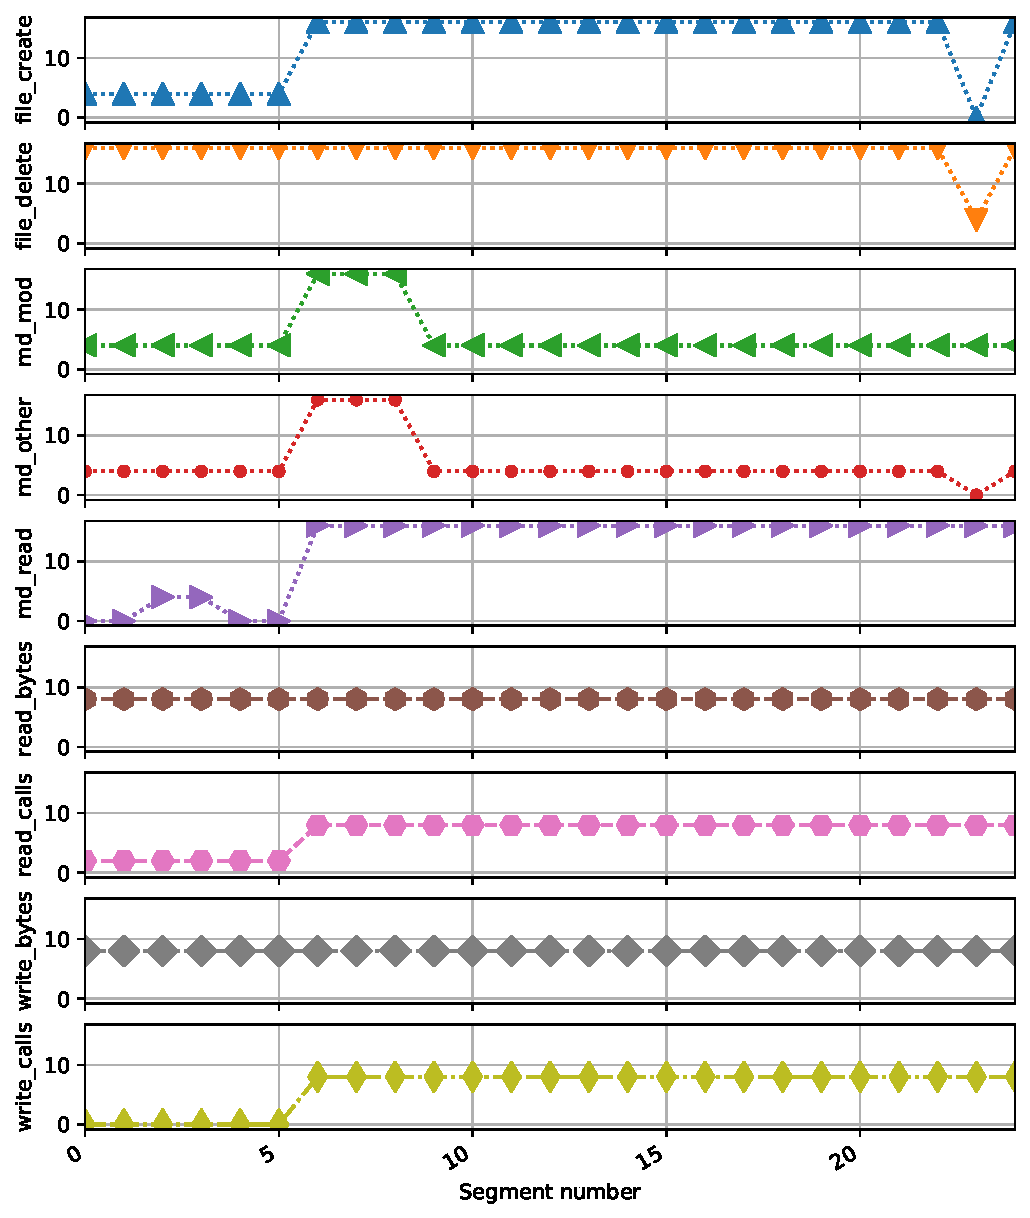
\includegraphics[width=\textwidth]{job-timeseries4296426}
\caption{Job-S (runtime=15,551\,s, segments=25)}\label{fig:job-S}
\end{subfigure}
\centering


\begin{subfigure}{0.8\textwidth}
\centering
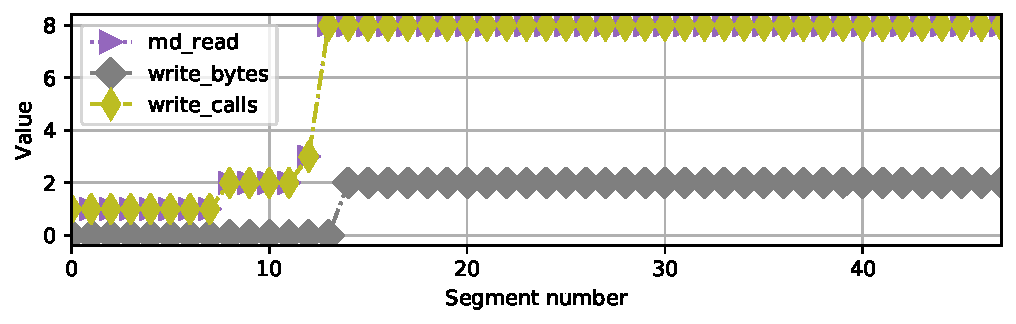
\includegraphics[width=\textwidth]{job-timeseries5024292}
\caption{Job-M (runtime=28,828\,s, segments=48)}\label{fig:job-M}
\end{subfigure}
\centering


\caption{Reference jobs: segmented timelines of mean I/O activity}%
\label{fig:refJobs}
\end{figure}


\begin{figure}\ContinuedFloat%

\begin{subfigure}{0.8\textwidth}
\centering
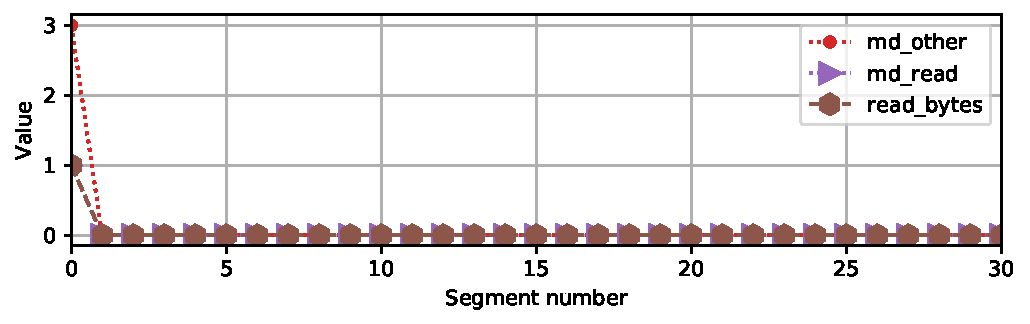
\includegraphics[width=\textwidth]{job-timeseries7488914-30}
\caption{Job-L (first 30 segments of 400; remaining segments are zero)}%
\label{fig:job-L}
\end{subfigure}
\centering
\caption{Reference jobs: segmented timelines of mean I/O activity}
\end{figure}


\begin{figure}
\begin{subfigure}{0.49\textwidth} % TODO war 0.8
\centering
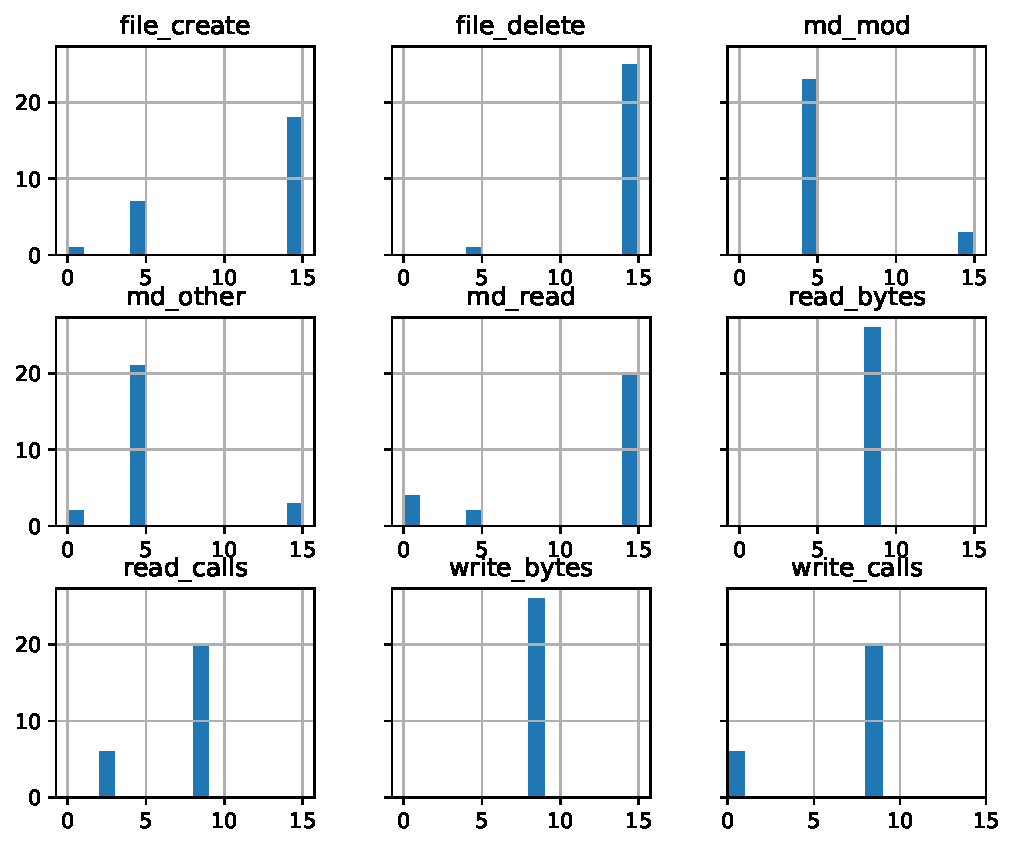
\includegraphics[width=\textwidth]{job-ks-0hist4296426}
\caption{Job-S}\label{fig:job-S-hist}
\end{subfigure}
\centering
\begin{subfigure}{0.49\textwidth}
\centering
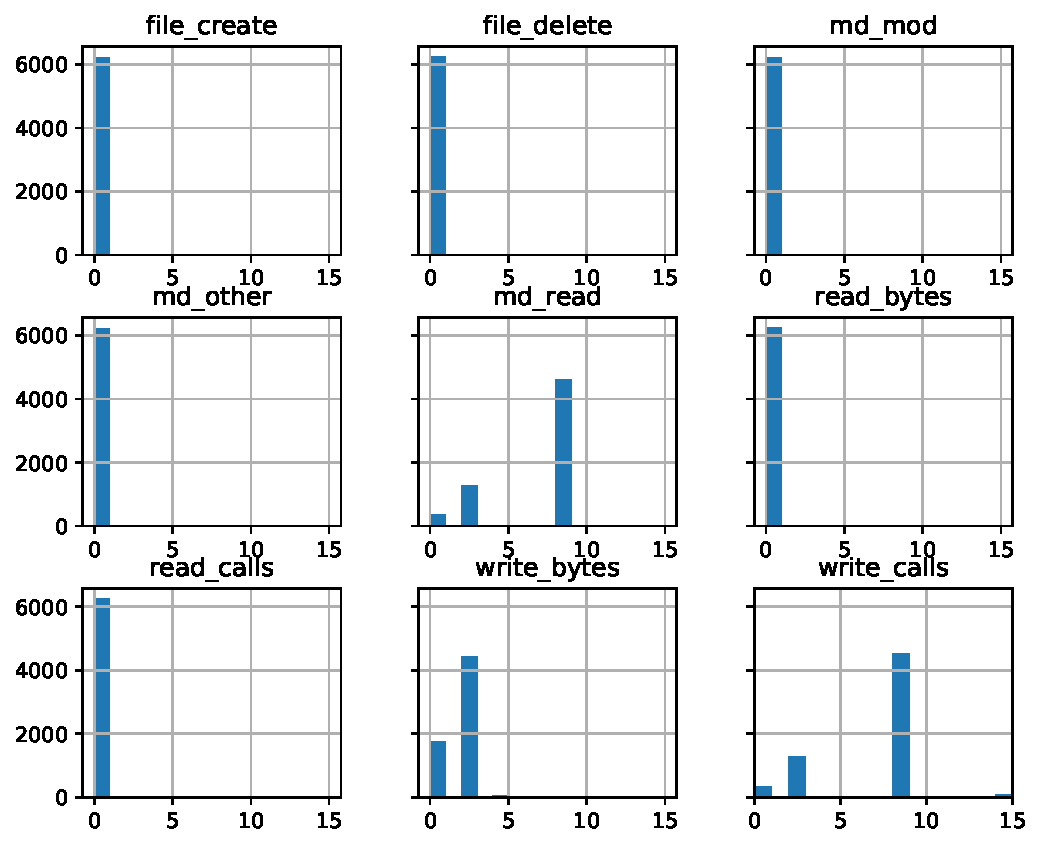
\includegraphics[width=\textwidth]{job-ks-1hist5024292}
\caption{Job-M}\label{fig:job-M-hist}
\end{subfigure}
\centering


\caption{Reference jobs: histogram of I/O activities}%
\label{fig:refJobsHist}
\end{figure}

%\begin{figure}\ContinuedFloat
%\begin{subfigure}{0.8\textwidth}
%\centering
%\includegraphics[width=\textwidth]{job-ks-2hist7488914}
%\caption{Job-L}
%\label{fig:job-L}
%\end{subfigure}
%\centering
%\caption{Reference jobs: histogram of I/O activities}
%\end{figure}



\section{Evaluation}%
\label{sec:evaluation}

In the following, we assume a reference job is given (we use Job-S, Job-M, and Job-L) and we aim to identify similar jobs.
For each reference job and algorithm, we created CSV files with the computed similarity to all other jobs from our job pool (worth 203 days of production of Mistral).
During this process, the runtime of the algorithm is recorded.
Then we inspect the correlation between the similarity and number of found jobs.
Finally, the quantitative behavior of the 100 most similar jobs is investigated.



\subsection{Performance}

To measure the performance for computing the similarity to the reference jobs, the algorithms are executed 10 times on a compute node at DKRZ which is equipped with two Intel Xeon E5-2680v3 @2.50GHz and 64GB DDR4 RAM.
A boxplot for the runtimes is shown in \Cref{fig:performance}.
The runtime is normalized for 100k jobs, i.e., for B-all it takes about 41\,s to process 100k jobs out of the 500k total jobs that this algorithm will process.
Generally, the B algorithms are fastest, while the Q algorithms often take 4-5x as long.
Q\_phases is slow for Job-S and Job-M while it is fast for Job-L. 
The reason is that just one phase is extracted for Job-L.
The Levenshtein based algorithms take longer for longer jobs -- proportional to the job length as it applies a sliding window.
The KS algorithm is faster than the others by 10x, but it operates on the statistics of the time series.
Note that the current algorithms are sequential and executed on just one core.
They could easily be parallelized which would then allow for an online analysis.

\begin{figure}
\centering
  \begin{subfigure}{0.48\textwidth}
  \centering
  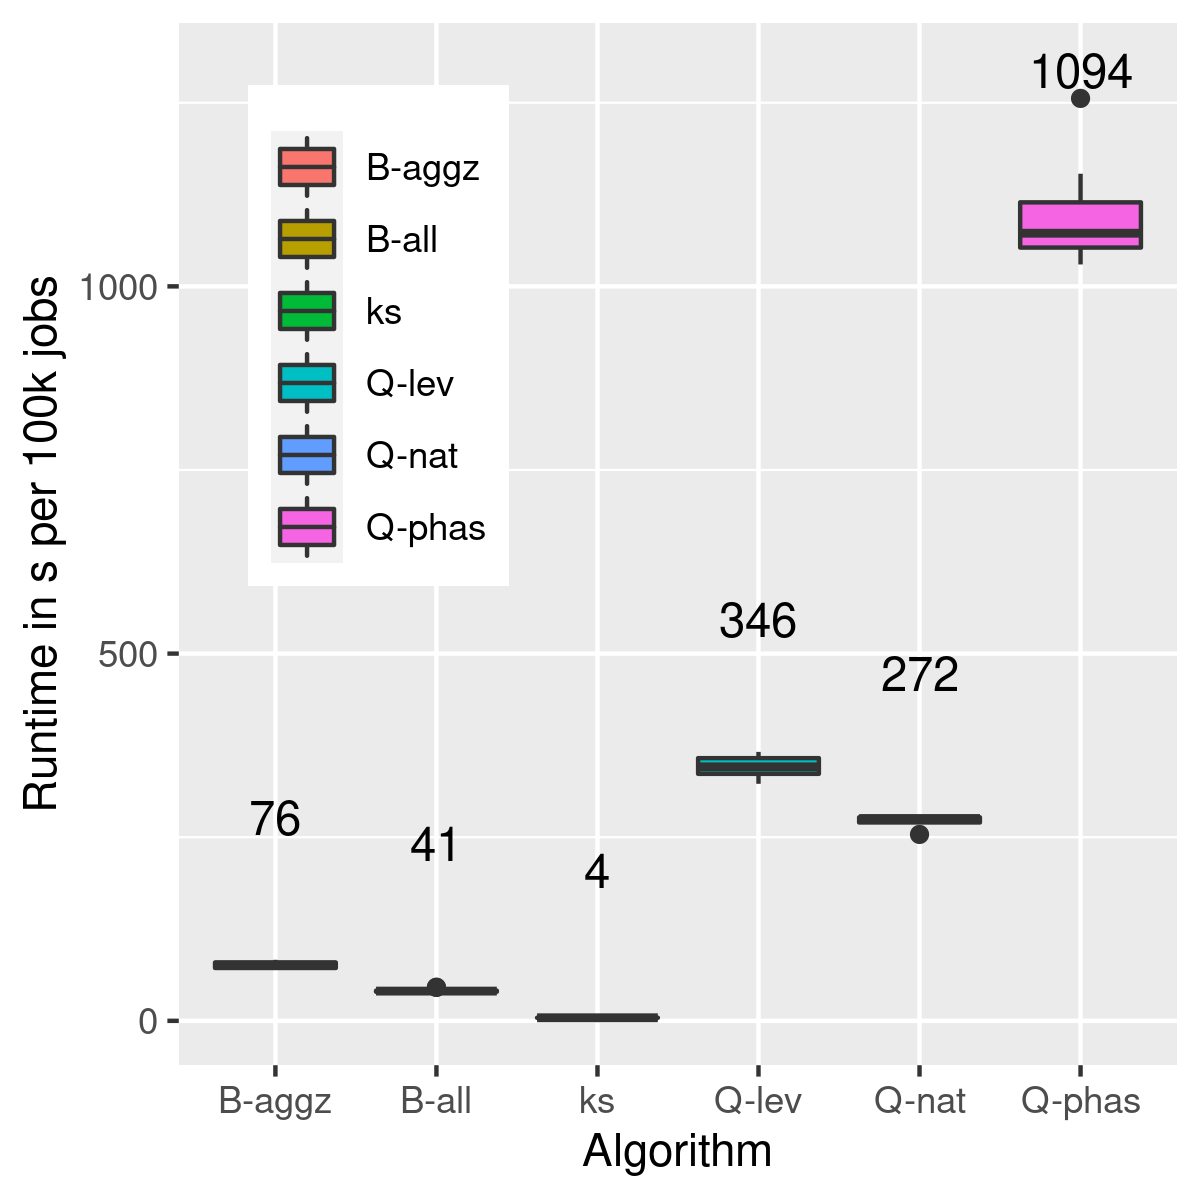
\includegraphics[width=\textwidth]{progress_4296426-out-boxplot}
  \caption{Job-S (segments=25)}\label{fig:perf-job-S}
  \end{subfigure}
  \begin{subfigure}{0.48\textwidth}
  \centering
  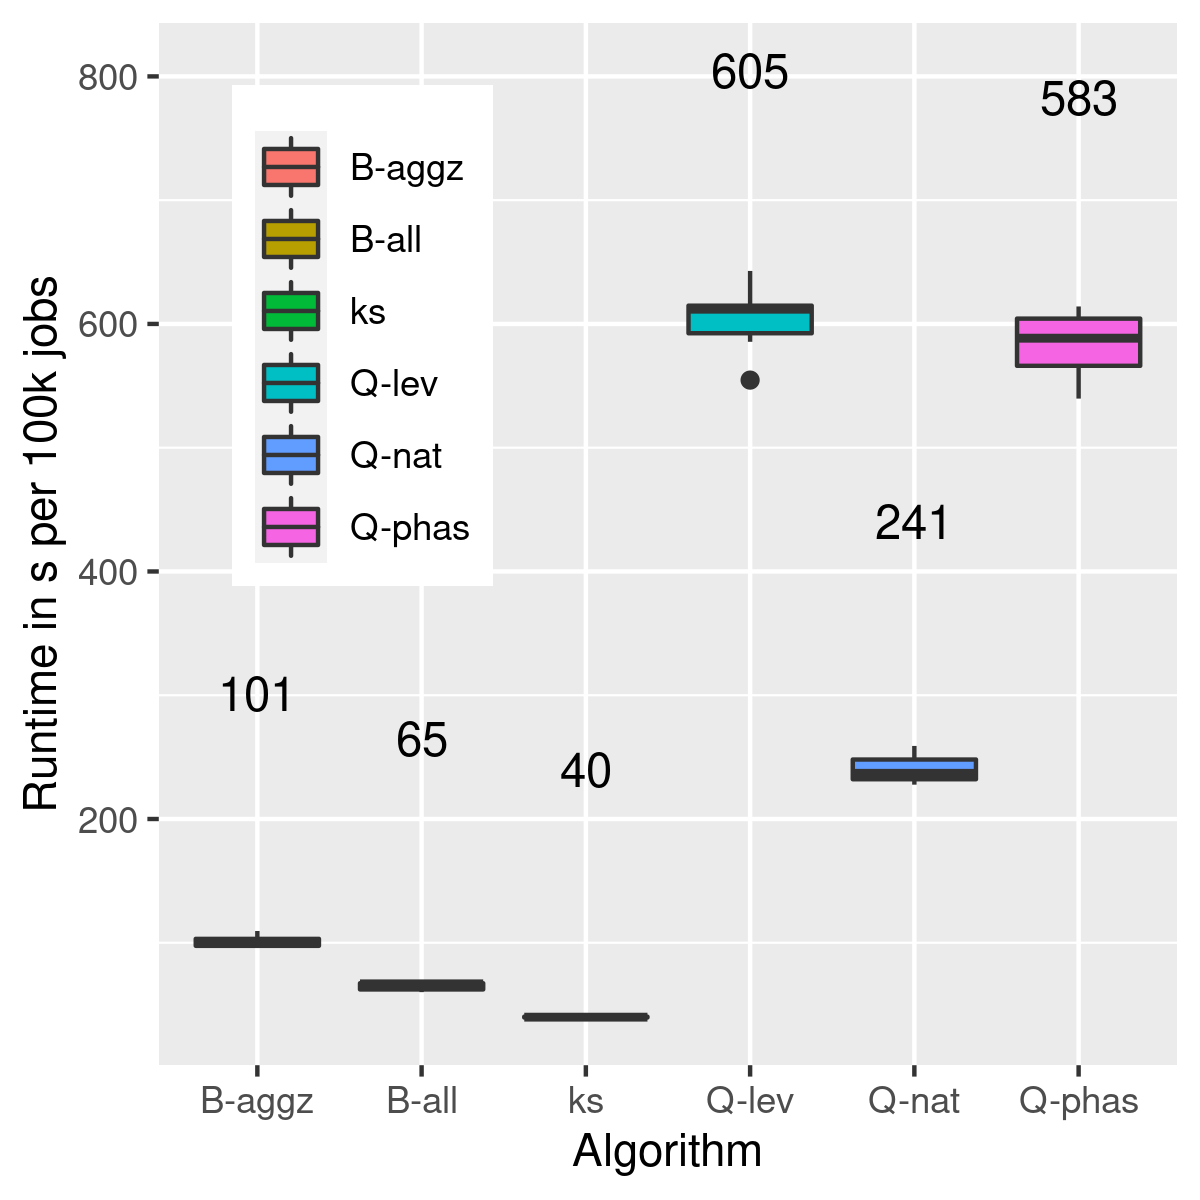
\includegraphics[width=\textwidth]{progress_5024292-out-boxplot}
  \caption{Job-M (segments=48)}\label{fig:perf-job-M}
  \end{subfigure}
  \begin{subfigure}{0.48\textwidth}
  \centering
  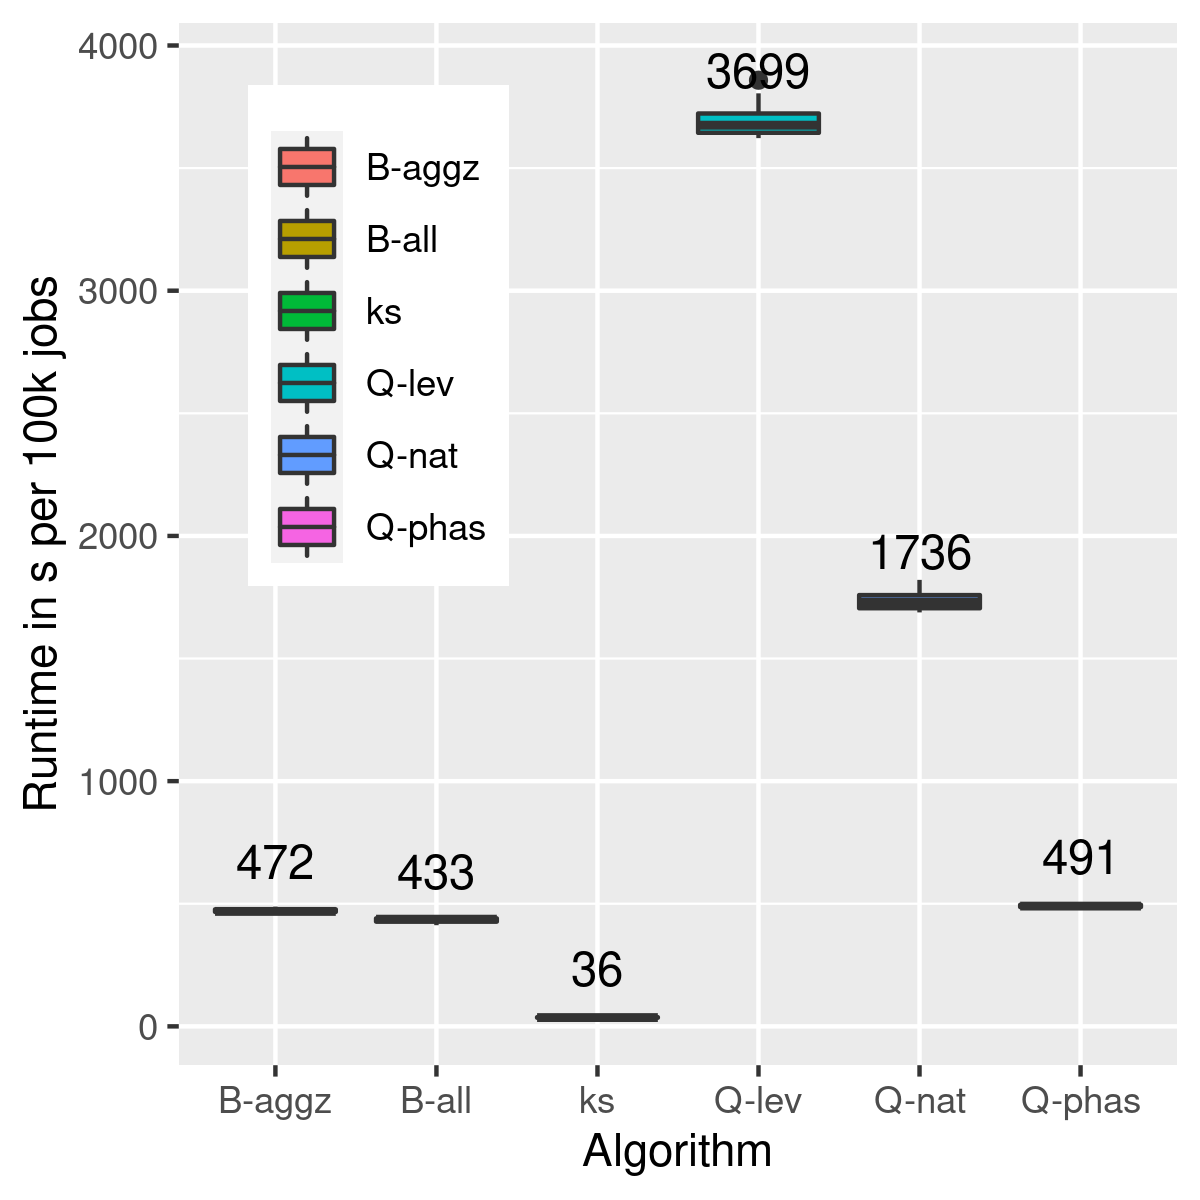
\includegraphics[width=\textwidth]{progress_7488914-out-boxplot}
  \caption{Job-L (segments=400)}\label{fig:perf-job-L}
  \end{subfigure}

  \caption{Runtime of the algorithms to compute the similarity to reference jobs}%
  \label{fig:performance}
\end{figure}


\subsection{Quantitative Analysis}

In the quantitative analysis, we explore the different algorithms how the similarity of our pool of jobs behaves to our reference jobs.
% TODO full paper
%The cumulative distribution of similarity to a reference job is shown in %\Cref{fig:ecdf}.
%For example, in \Cref{fig:ecdf-job-S}, we see that about 70\% have a similarity of less than 10\% to Job-S for Q-native.
%B-aggz shows some steep increases, e.g., more than 75\% of jobs have the same low similarity below 2\%.
%The different algorithms lead to different curves for our reference jobs, e.g., for Job-S, Q-phases bundles more jobs with low similarity compared to the other jobs; in Job-L, it is the slowest.
% This indicates that the algorithms
The support team in a data center may have time to investigate the most similar jobs.
Time for the analysis is typically bound, for instance, the team may analyze the 100 most similar jobs and rank them; we refer to them as the Top\,100 jobs, and \textit{Rank\,i} refers to the job that has the i-th highest similarity to the reference job -- sometimes these values can be rather close together as we see in the histogram in
\Cref{fig:hist} for the actual number of jobs with a given similarity.
As we focus on a feasible number of jobs, we crop it at 100 jobs (total number of jobs is still given).
It turns out that both B algorithms produce nearly identical histograms, and we omit one of them.
In the figures, we can see again a different behavior of the algorithms depending on the reference job.
Especially for Job-S, we can see clusters with jobs of higher similarity (e.g., at Q-lev at SIM=75\%) while for Job-M, the growth in the relevant section is more steady.
For Job-L, we find barely similar jobs, except when using the Q-phases and KS algorithms.
Q-phases find 393 jobs that have a similarity of 100\%, thus they are indistinguishable, while KS identifies 6880 jobs with a similarity of at least 97.5\%.
Practically, the support team would start with Rank\,1 (most similar job, e.g., the reference job) and walk down until the jobs look different, or until a cluster of jobs with close similarity is analyzed.

%  TODO full paper?
% \begin{figure}
%
% \begin{subfigure}{0.8\textwidth}
% \centering
% \includegraphics[width=\textwidth]{job_similarities_4296426-out/ecdf}
% \caption{Job-S} \label{fig:ecdf-job-S}
% \end{subfigure}
% \centering
%
% \begin{subfigure}{0.8\textwidth}
% \centering
% \includegraphics[width=\textwidth]{job_similarities_5024292-out/ecdf}
% \caption{Job-M} \label{fig:ecdf-job-M}
% \end{subfigure}
% \centering
%
% \begin{subfigure}{0.8\textwidth}
% \centering
% \includegraphics[width=\textwidth]{job_similarities_7488914-out/ecdf}
% \caption{Job-L} \label{fig:ecdf-job-L}
% \end{subfigure}
% \centering
% \caption{Quantitative job similarity -- empirical cumulative density function}
% \label{fig:ecdf}
% \end{figure}


\begin{figure}
\centering

\begin{subfigure}{0.67\textwidth}
\centering
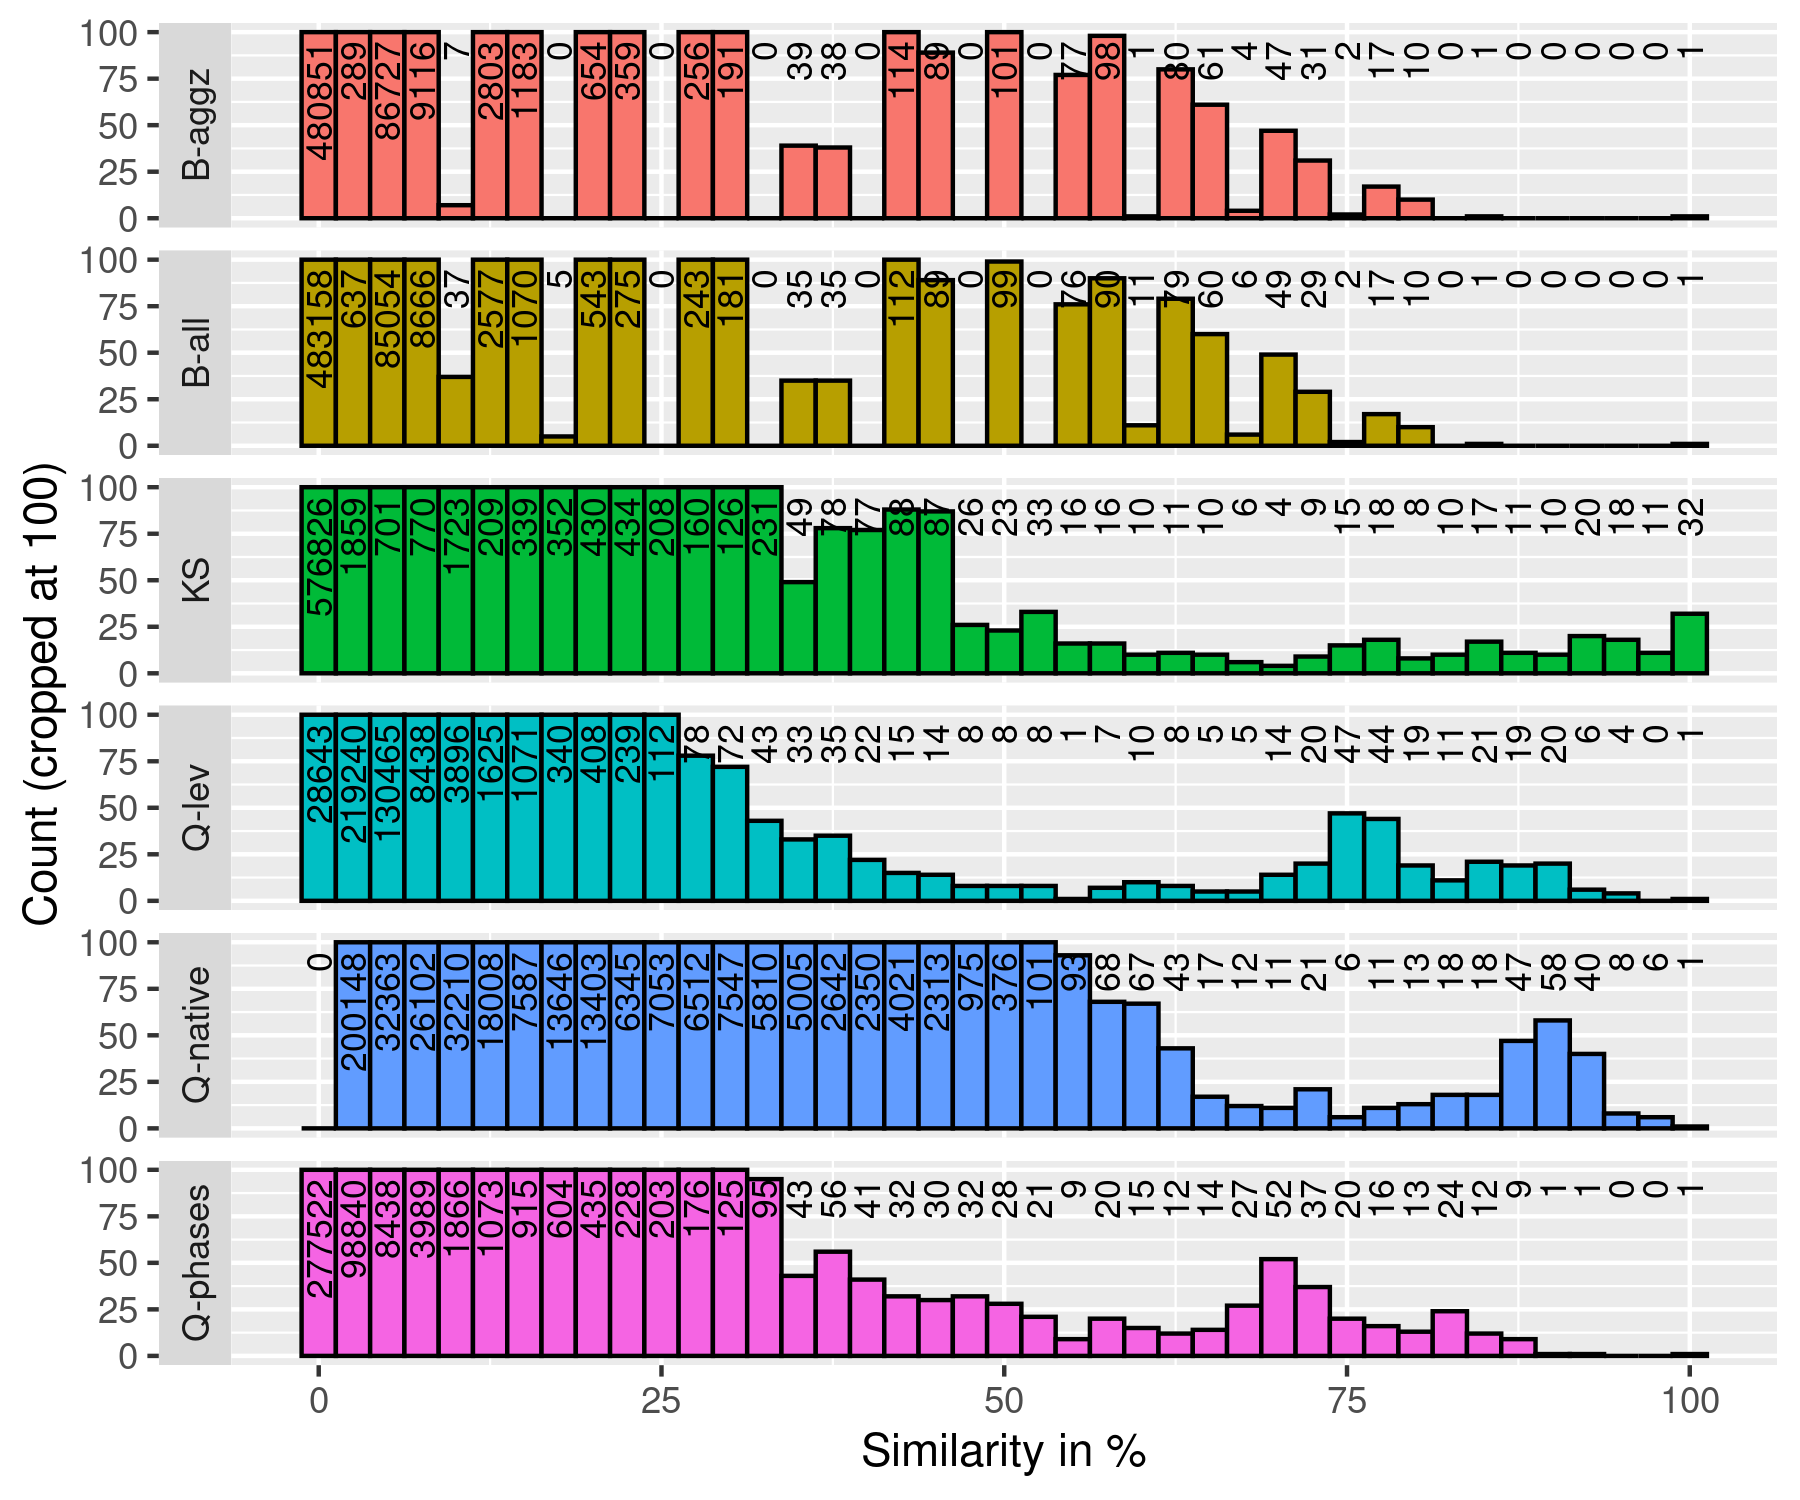
\includegraphics[width=\textwidth,trim={0 0 0 2.0cm},clip]{job_similarities_4296426-out/hist-sim}
\caption{Job-S}\label{fig:hist-job-S}
\end{subfigure}

\begin{subfigure}{0.67\textwidth}
\centering
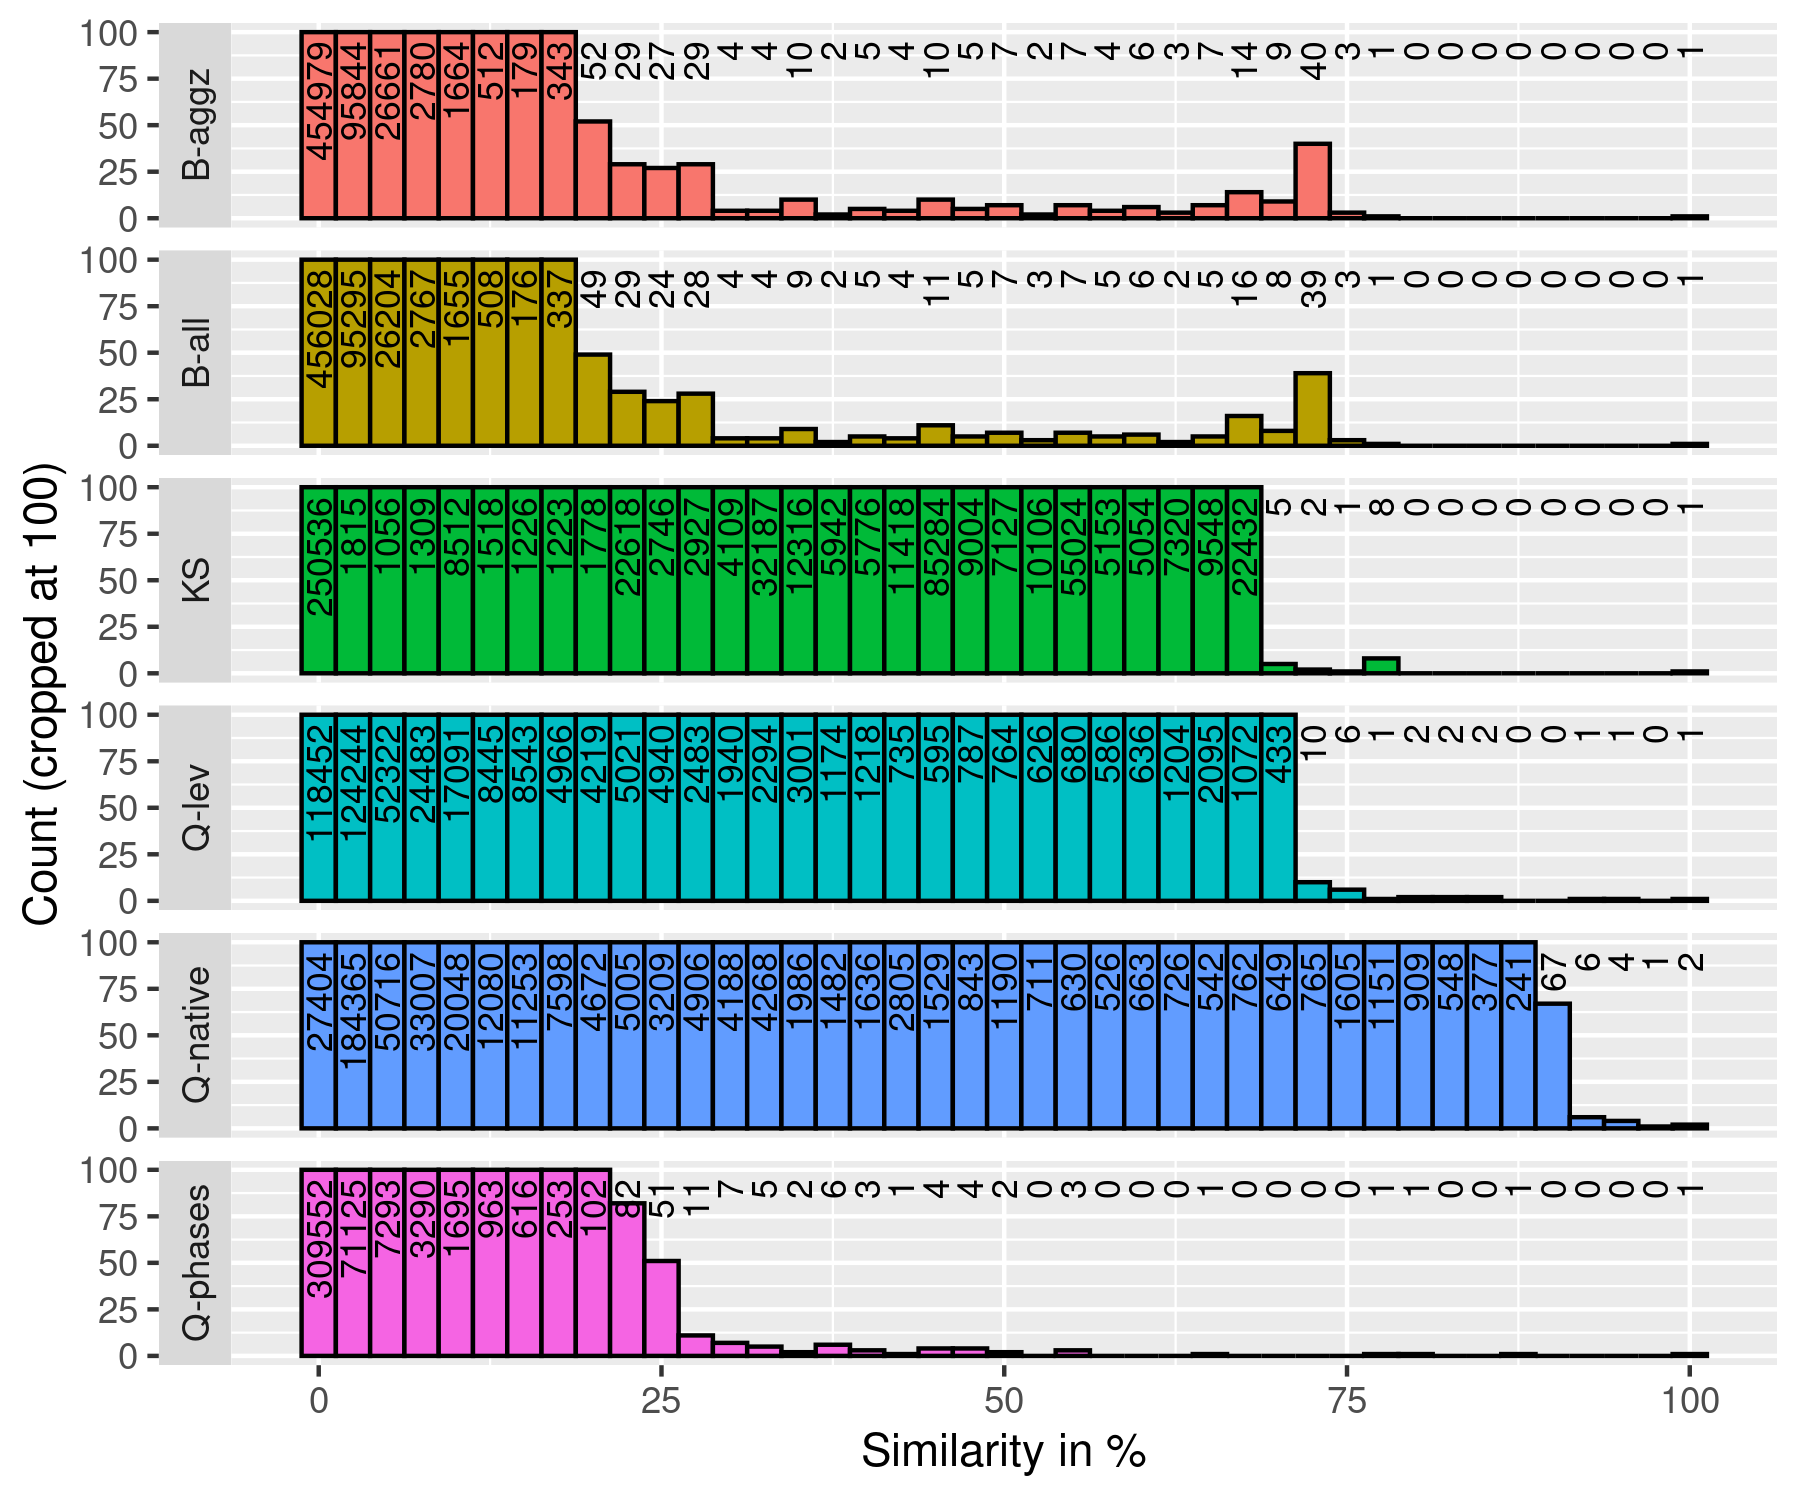
\includegraphics[width=\textwidth,trim={0 0 0 2.0cm},clip]{job_similarities_5024292-out/hist-sim}
\caption{Job-M}\label{fig:hist-job-M}
\end{subfigure}

\begin{subfigure}{0.67\textwidth}
\centering
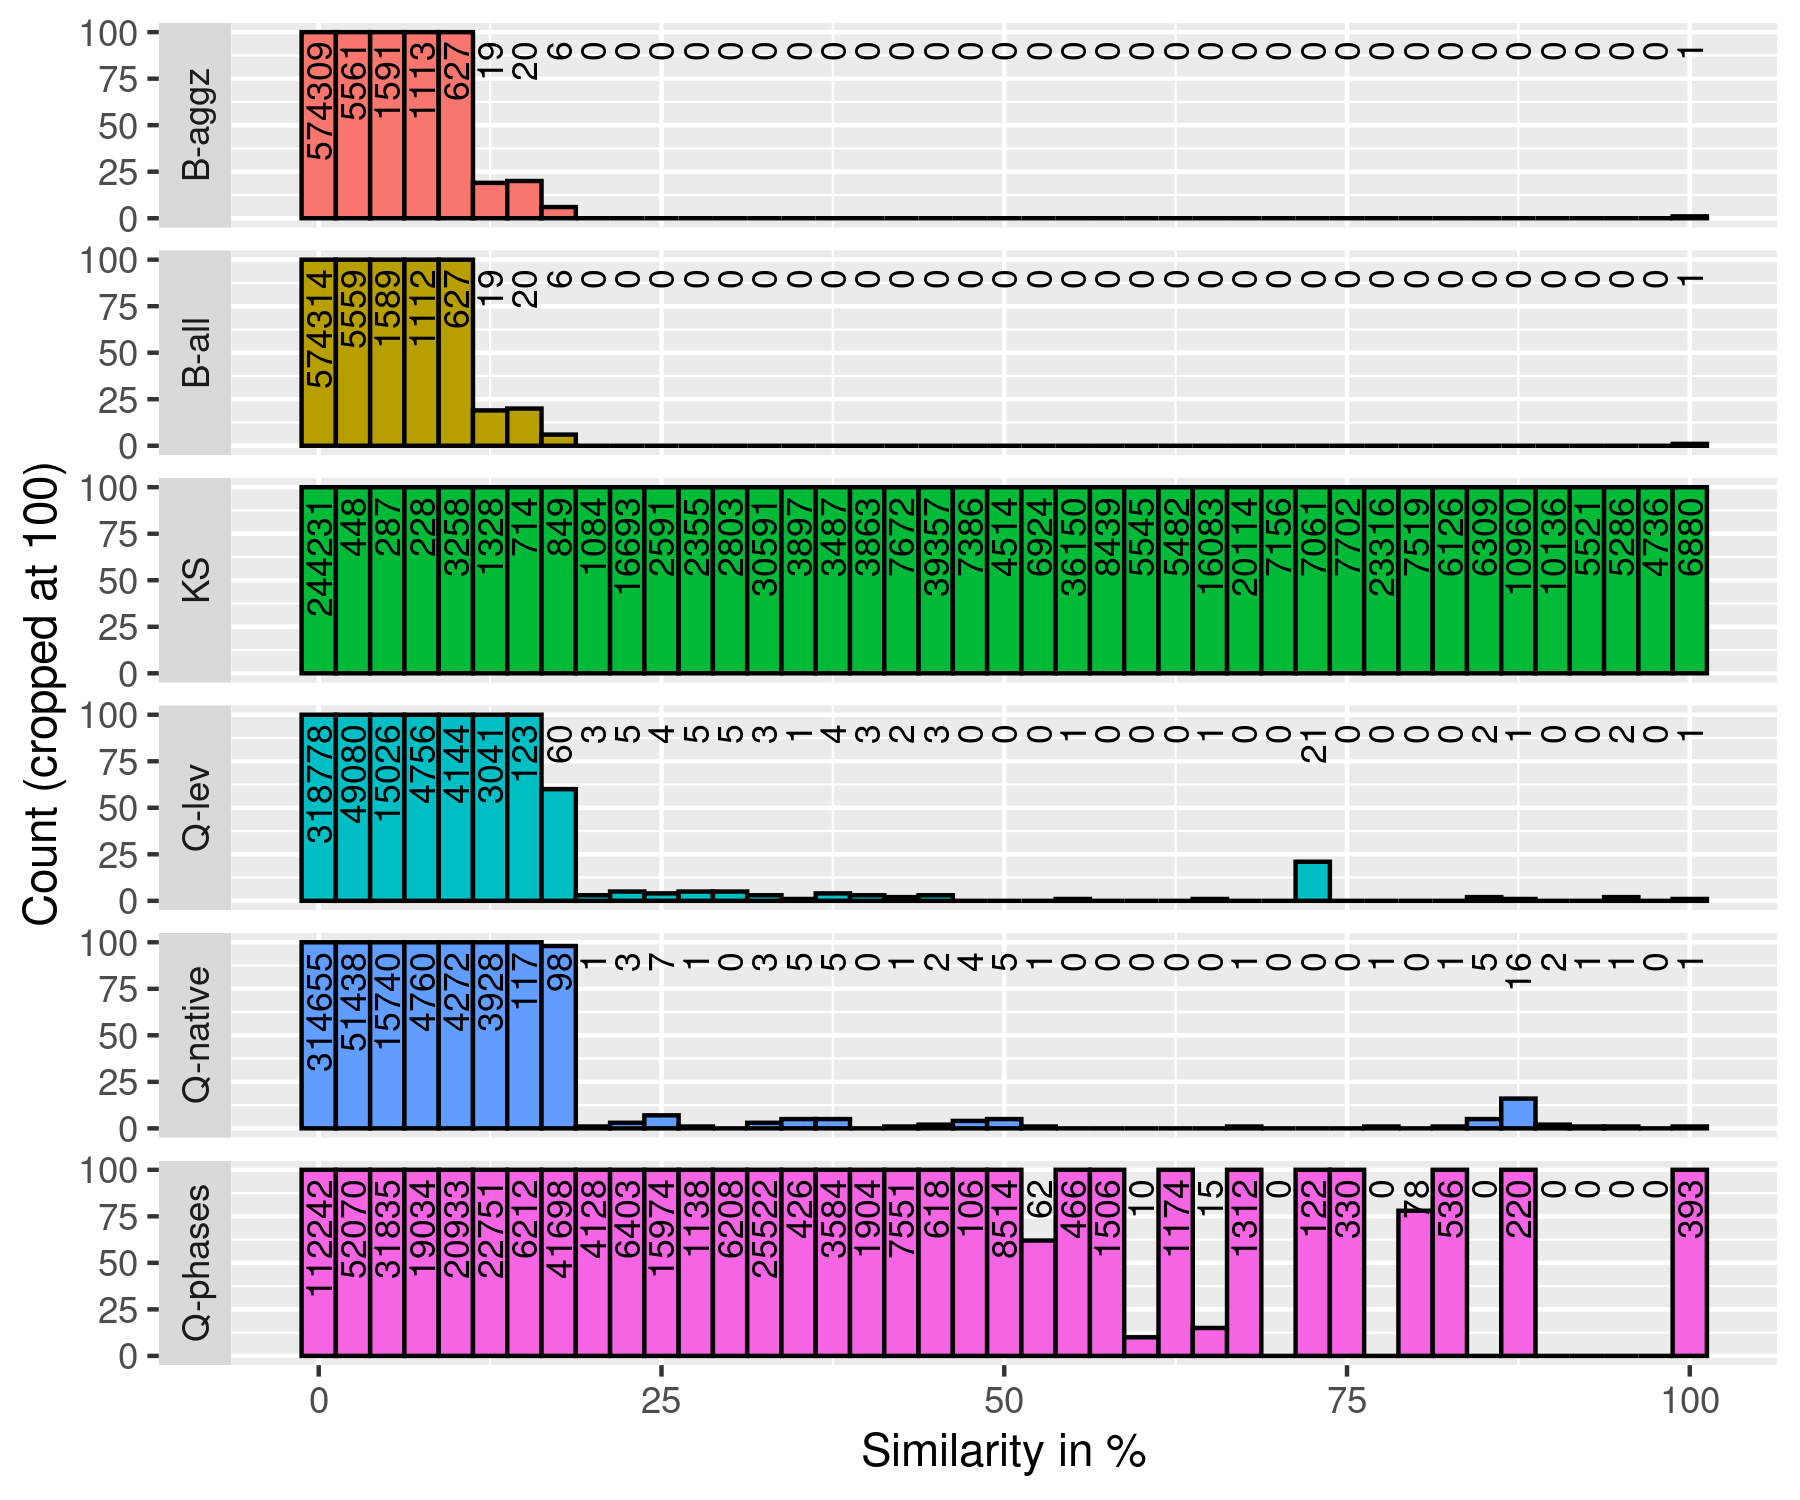
\includegraphics[width=\textwidth,trim={0 0 0 2.0cm},clip]{job_similarities_7488914-out/hist-sim}
\caption{Job-L}\label{fig:hist-job-L}
\end{subfigure}
\centering
\caption{Histogram for the number of jobs (bin width: 2.5\%, numbers are the actual job counts). B-aggz is nearly identical to B-all and therefore omitted.}%
\label{fig:hist}
\end{figure}

\subsubsection{Inclusivity and Specificity}

When analyzing the overall population of jobs executed on a system, we expect that some workloads are executed several times (with different inputs but with the same configuration) or are executed with slightly different configurations (e.g., node counts, timesteps).
Thus, potentially our similarity analysis of the job population may just identify the re-execution of the same workload.
Typically, the support staff would identify the re-execution of jobs by inspecting job names which are user-defined generic strings%\footnote{%
%As they can contain confidential data, it is difficult to anonymize them without perturbing the meaning.
%Therefore, they are not published in our data repository.
%}

To understand if the analysis is inclusive and identifies different applications, we use two approaches with our Top\,100 jobs:
We explore the distribution of users (and groups), runtime, and node count across jobs.
The algorithms should include different users, node counts, and across runtime.
To confirm the hypotheses presented, we analyzed the job metadata comparing job names which validate our quantitative results discussed in the following.


\paragraph{User distribution.}
To understand how the Top\,100 are distributed across users, the data is grouped by userid and counted.
\Cref{fig:userids} shows the stacked user information, where the lowest stack is the user with the most jobs and the topmost user in the stack has the smallest number of jobs.
For Job-S, we can see that about 70-80\% of jobs stem from one user, for the Q-lev and Q-native algorithms, the other jobs stem from a second user while B algorithms include jobs from additional users (5 in total).
For Job-M, jobs from more users are included (13); about 25\% of jobs stem from the same user; here, Q-lev, Q-native, and KS include more users (29, 33, and 37, respectively) than the other three algorithms.
For Job-L, the two Q algorithms include (12 and 13) a bit more diverse user community than the B algorithms (9) but Q-phases cover 35 users.
We didn't include the group analysis in the figure as user count and group id is proportional, at most the number of users is 2x the number of groups.
Thus, a user is likely from the same group and the number of groups is similar to the number of unique users.

\paragraph{Node distribution.}
\Cref{fig:nodes-job} shows a boxplot for the node counts in the Top\,100 -- the red line marks the reference job.
All algorithms reduce over the node dimensions, therefore, we naturally expect a big inclusion across the node range as long as the average I/O behavior of the jobs is similar.
For Job-M and Job-L, we can observe that indeed the range of similar nodes is between 1 and 128.
For Job-S, all 100 top-ranked jobs use one node.
As post-processing jobs use typically one node and the number of post-processing jobs is a high proportion, it appears natural that all Top\,100 are from this class of jobs, which is confirmed by investigating the job metadata.
The boxplots have different shapes which is an indication that the different algorithms identify a different set of jobs -- we will analyze this later further.

\paragraph{Runtime distribution.}
The job runtime of the Top\,100 jobs is shown using boxplots in \Cref{fig:runtime-job}.
While all algorithms can compute the similarity between jobs of different length, the B algorithms and Q-native penalize jobs of different length preferring jobs of very similar length.
For Job-M and Job-L, Q-phases and KS are able to identify much shorter or longer jobs.
For Job-L, for Q-phases and KS, the job itself isn't included in the chosen Top\,100 (see \Cref{fig:hist-job-L}, 393 jobs have a similarity of 100\%) which is the reason why the job runtime isn't shown in the figure itself.
Also, as there are only few jobs of similar lengths to Job-L and the B-* algorithms penalize job-length differences, the Top\,100 similar jobs have a significant difference in job length.

\begin{figure}[bt]
\begin{subfigure}{0.48\textwidth}
\centering
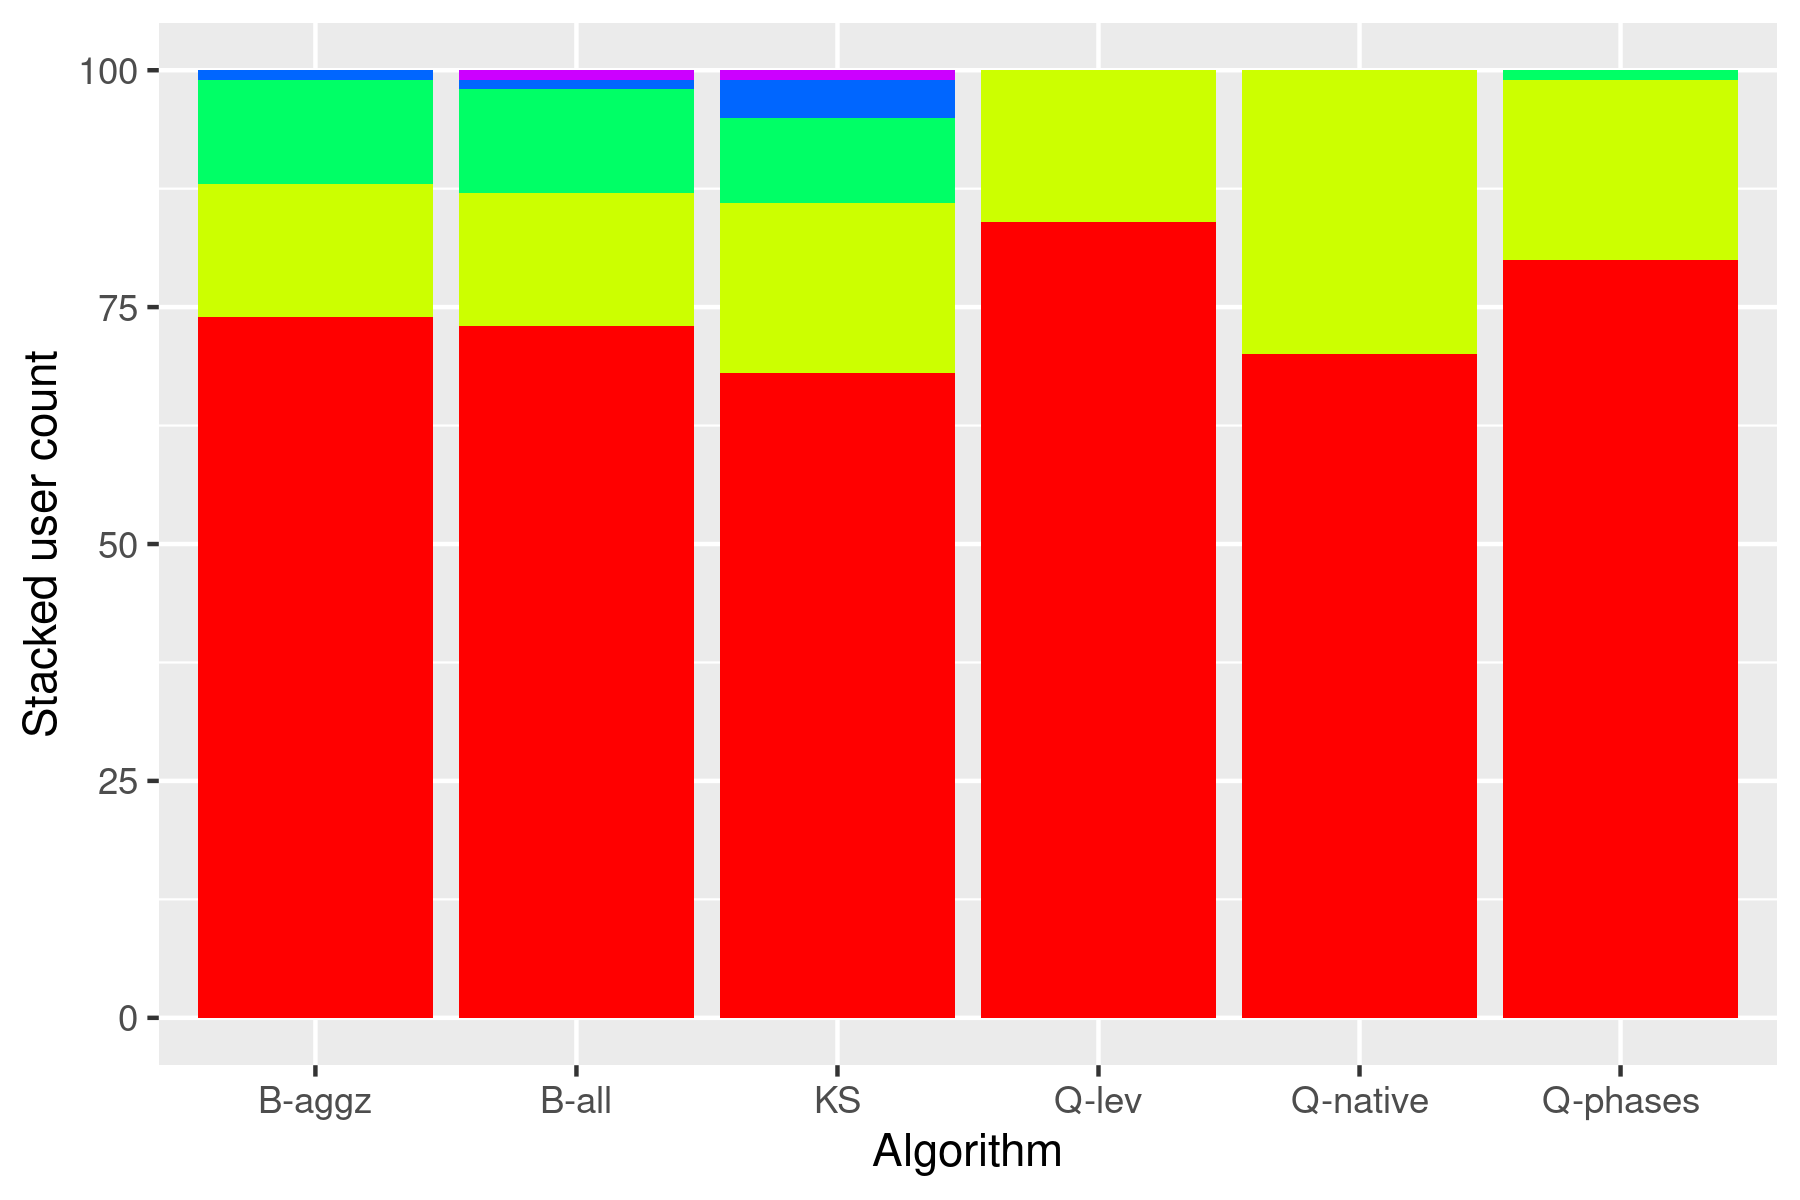
\includegraphics[width=\textwidth]{job_similarities_4296426-out/user-ids}
\caption{Job-S}\label{fig:users-job-S}
\end{subfigure}
\begin{subfigure}{0.48\textwidth}
\centering
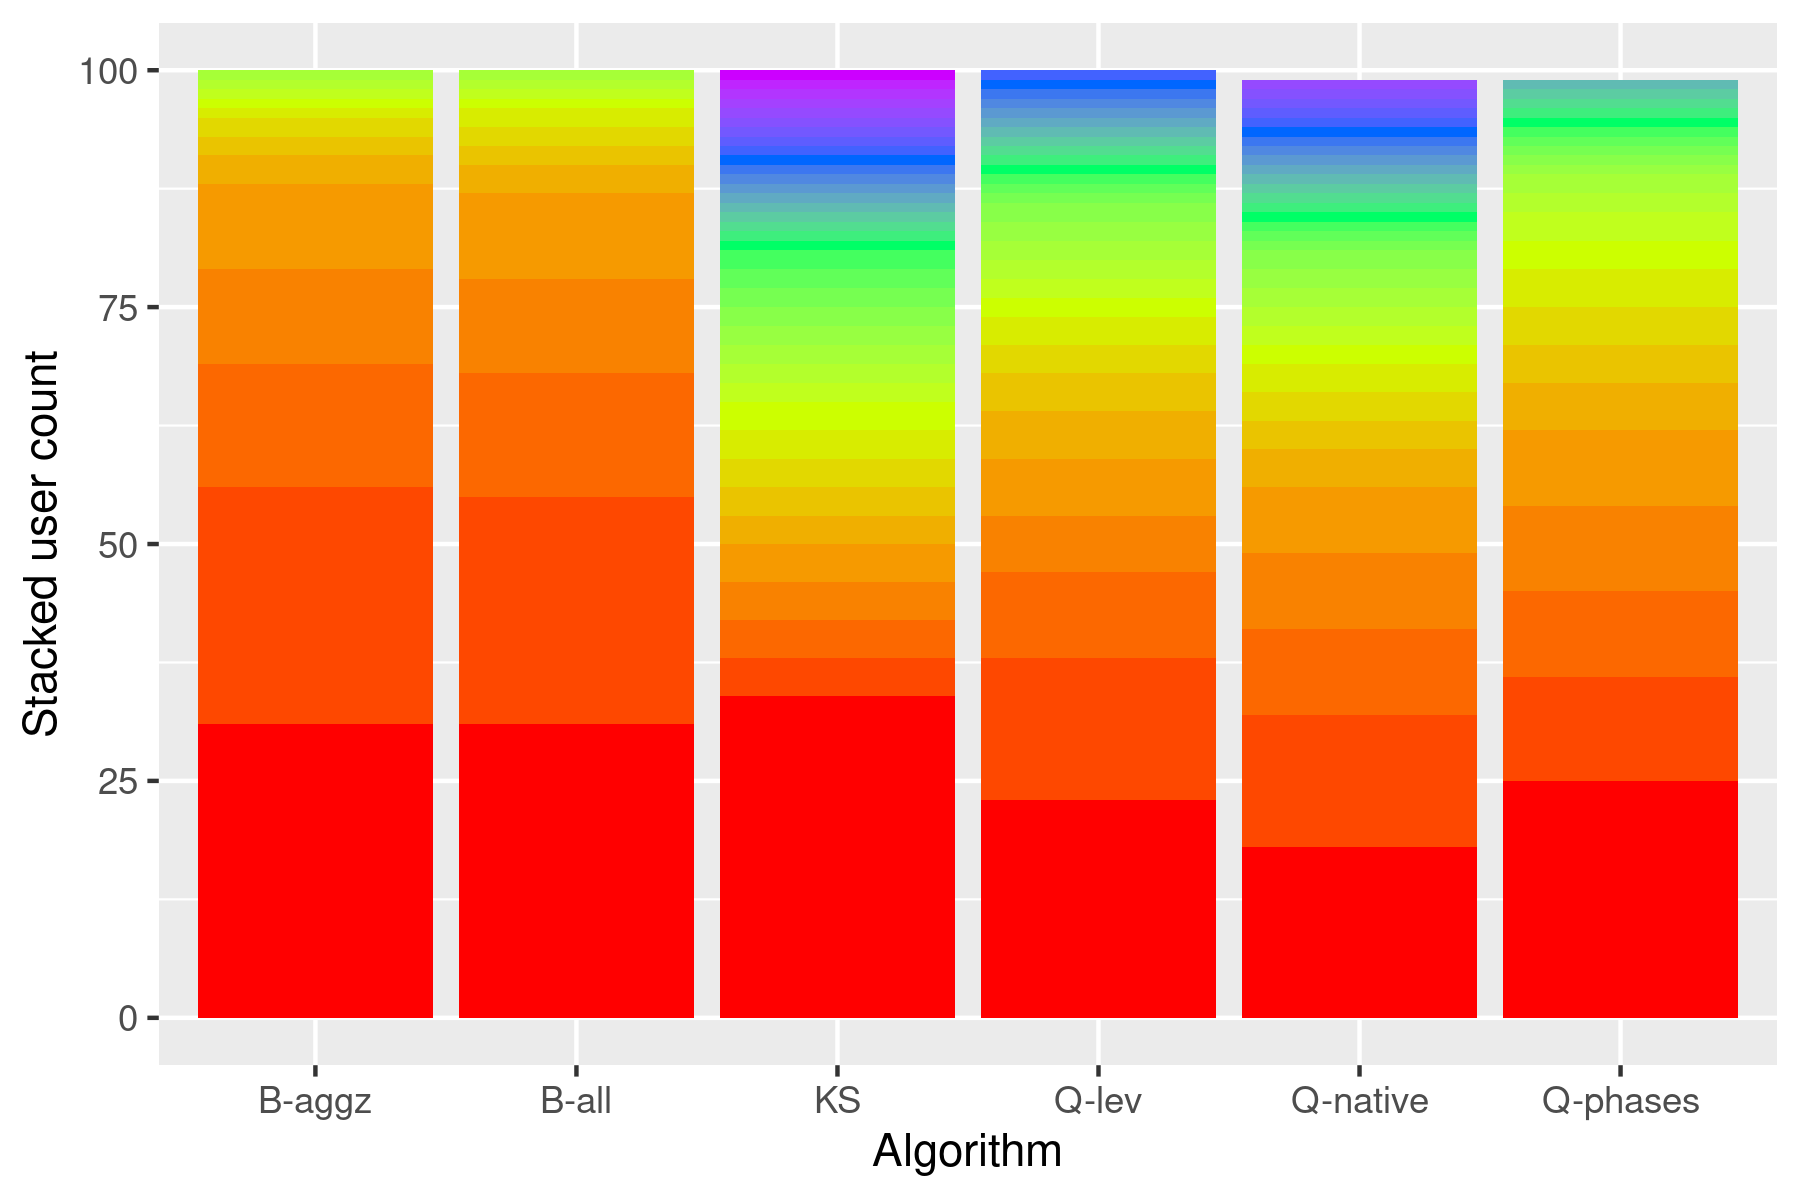
\includegraphics[width=\textwidth]{job_similarities_5024292-out/user-ids}
\caption{Job-M}\label{fig:users-job-M}
\end{subfigure}
\begin{subfigure}{0.48\textwidth}
\centering
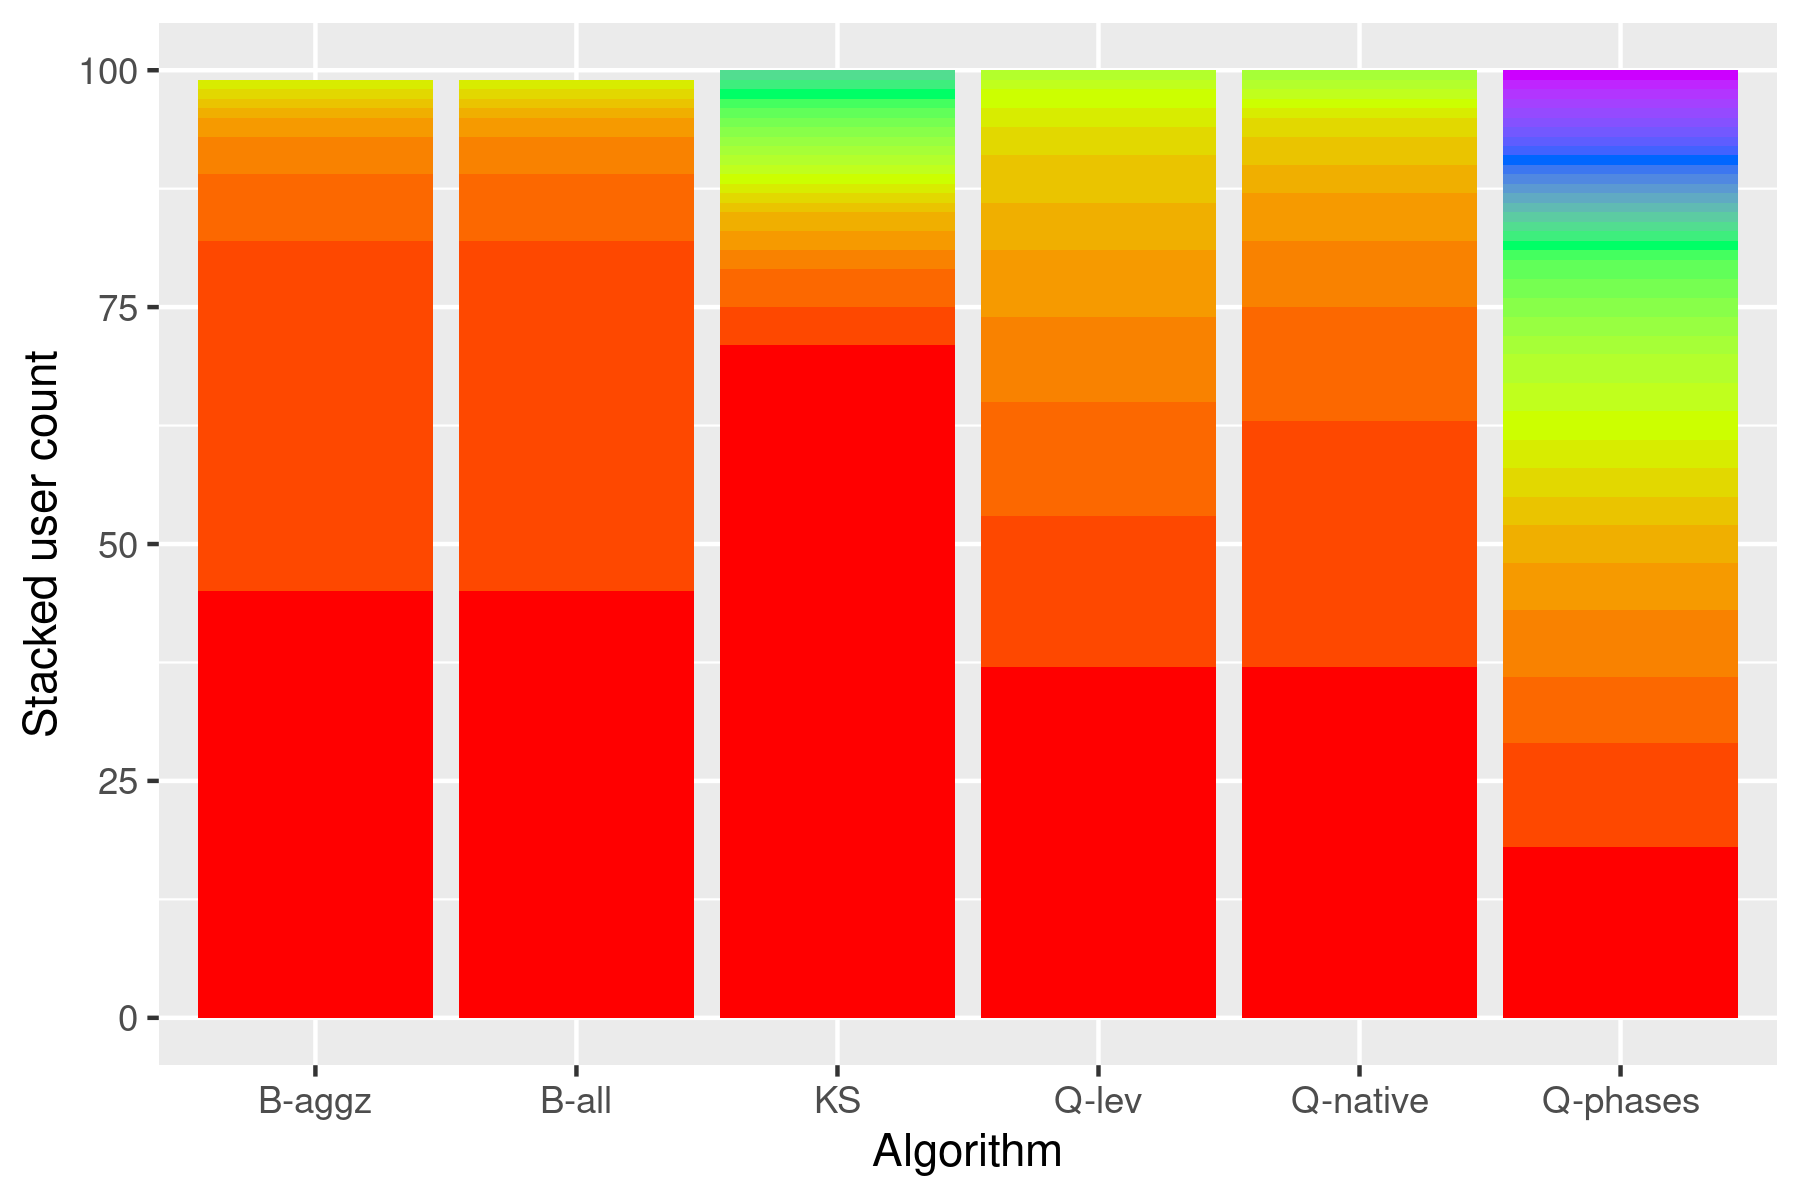
\includegraphics[width=\textwidth]{job_similarities_7488914-out/user-ids}
\caption{Job-L}\label{fig:users-job-L}
\end{subfigure}

\caption{User information for all 100 top-ranked jobs. Each color represents a specific user for the given data.}
\label{fig:userids}
\end{figure}

\begin{figure}
%\begin{subfigure}{0.31\textwidth}
%\centering
%\includegraphics[width=\textwidth]{job_similarities_4296426-out/jobs-nodes}
%\caption{Job-S} \label{fig:nodes-job-S}
%\end{subfigure}
\begin{subfigure}{0.48\textwidth}
\centering
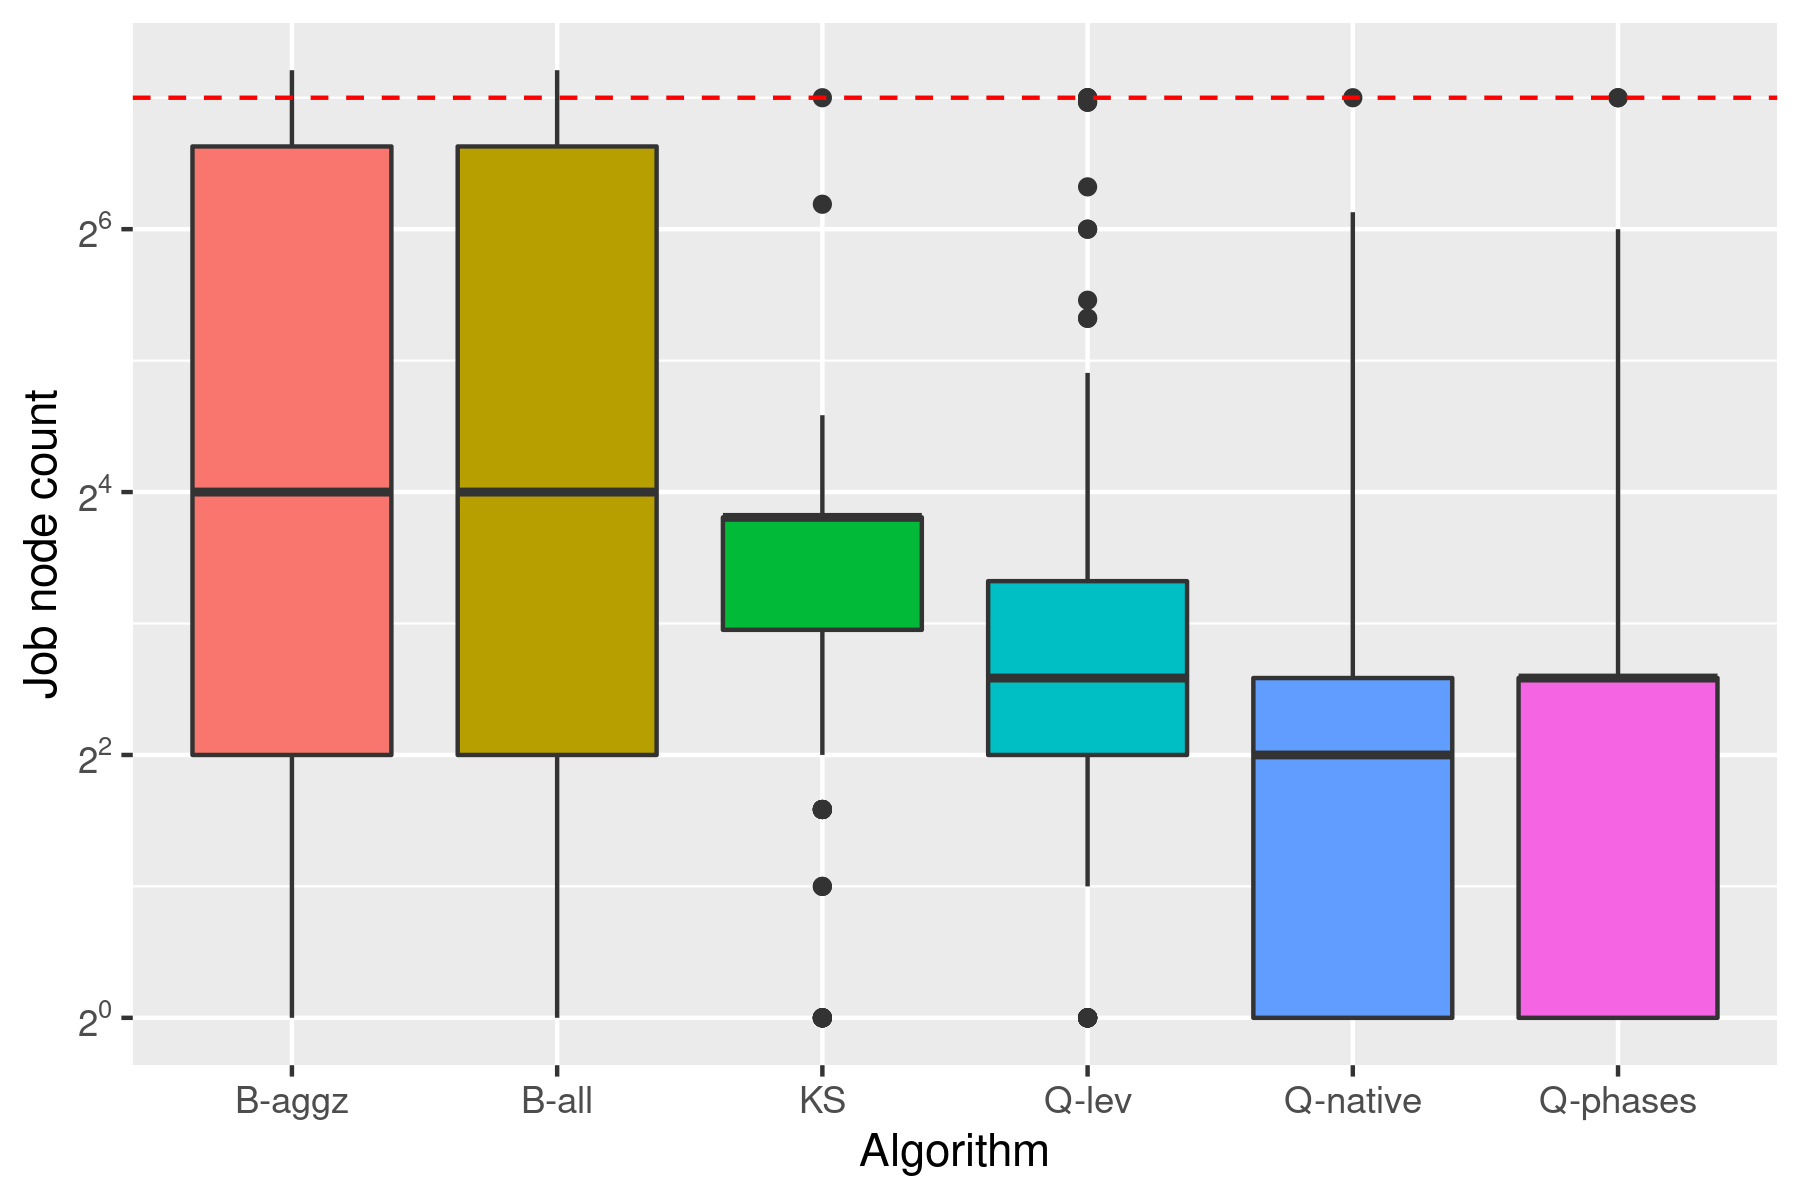
\includegraphics[width=\textwidth]{job_similarities_5024292-out/jobs-nodes}
\caption{Job-M (ref. job runs on 128 nodes)}\label{fig:nodes-job-M}
\end{subfigure}
\begin{subfigure}{0.48\textwidth}
\centering
\includegraphics[width=\textwidth]{job_similarities_7488914-out/jobs-nodes}
\caption{Job-L (reference job runs on 20 nodes)}\label{fig:nodes-job-L}
\end{subfigure}
\centering
\caption{Distribution of node counts for Top 100 (for Job-S always nodes=1)}%
\label{fig:nodes-job}
\end{figure}

\begin{figure}
\begin{subfigure}{0.7\textwidth}
\centering
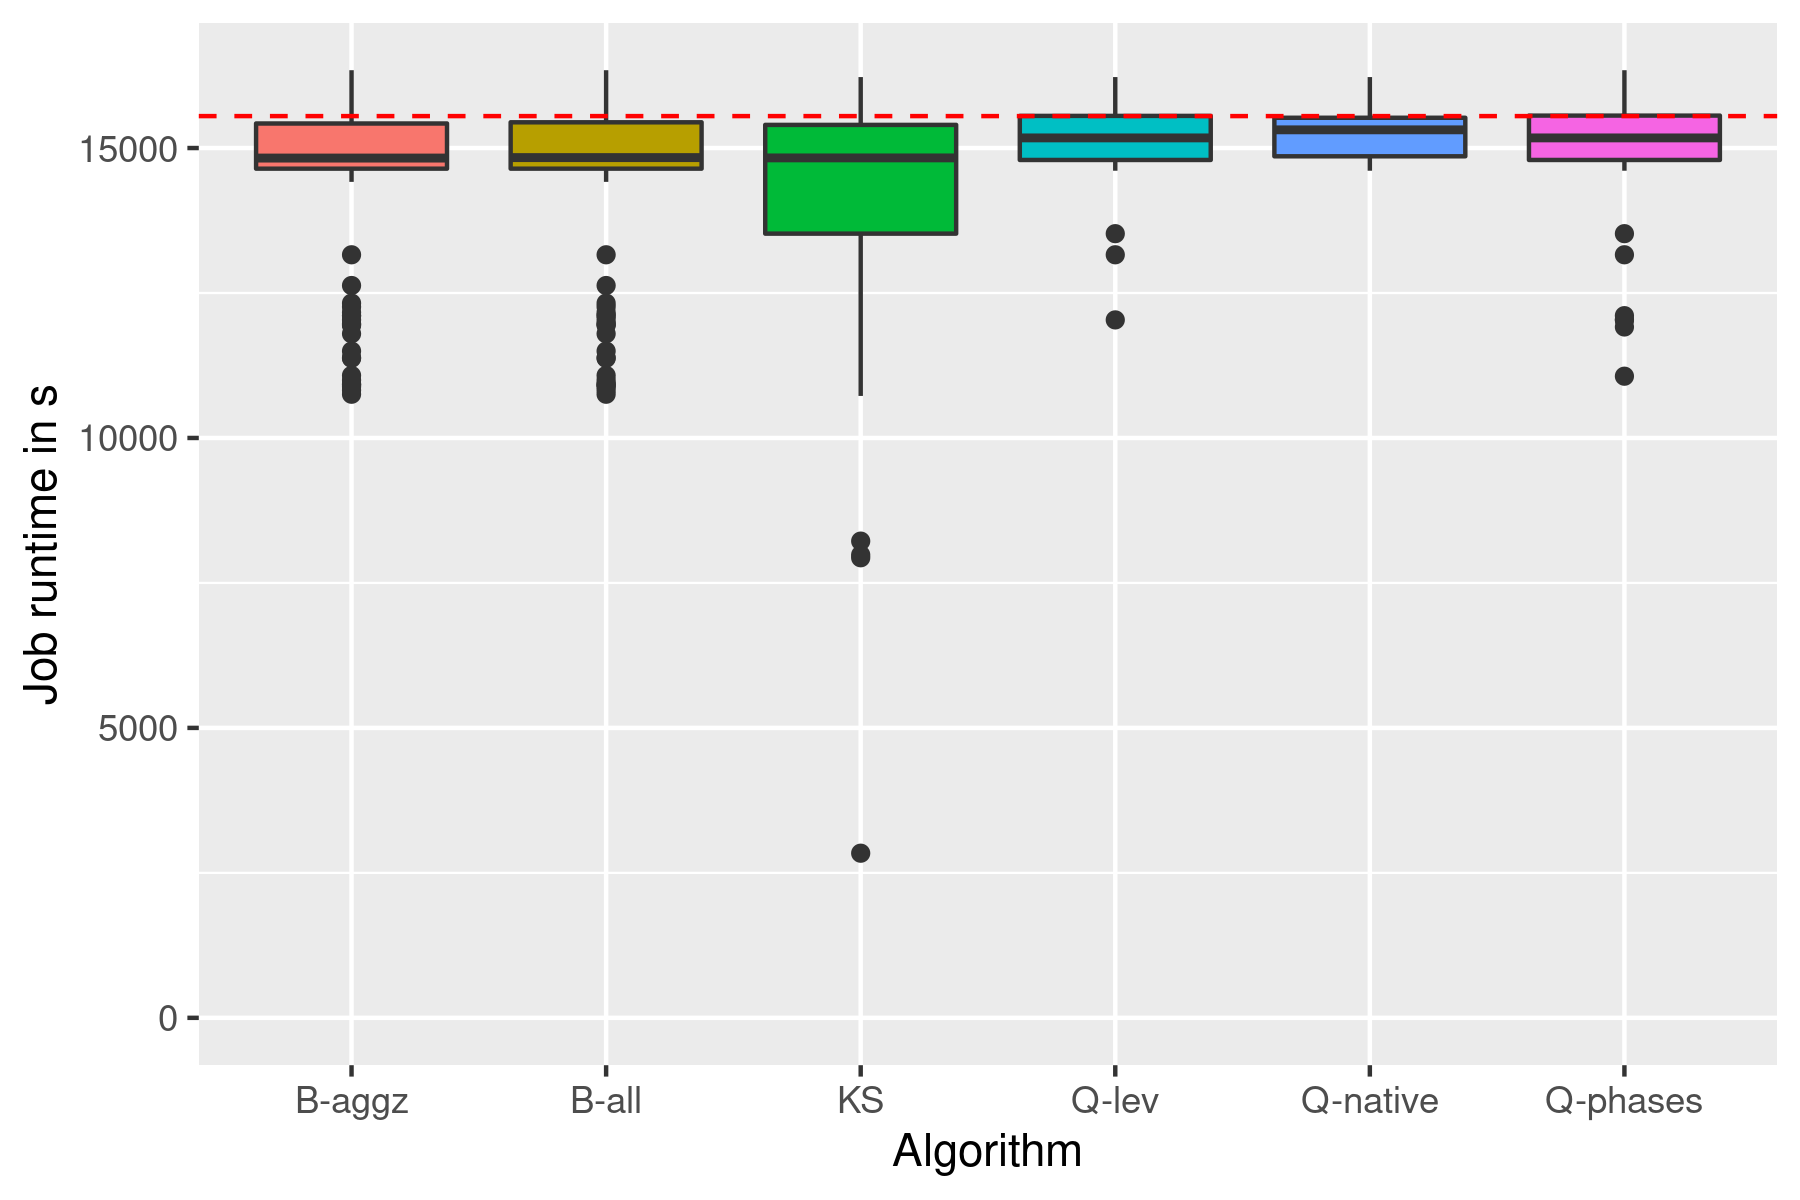
\includegraphics[width=\textwidth]{job_similarities_4296426-out/jobs-elapsed}
\caption{Job-S ($job=15,551s$)}\label{fig:runtime-job-S}
\end{subfigure}
\begin{subfigure}{0.7\textwidth}
\centering
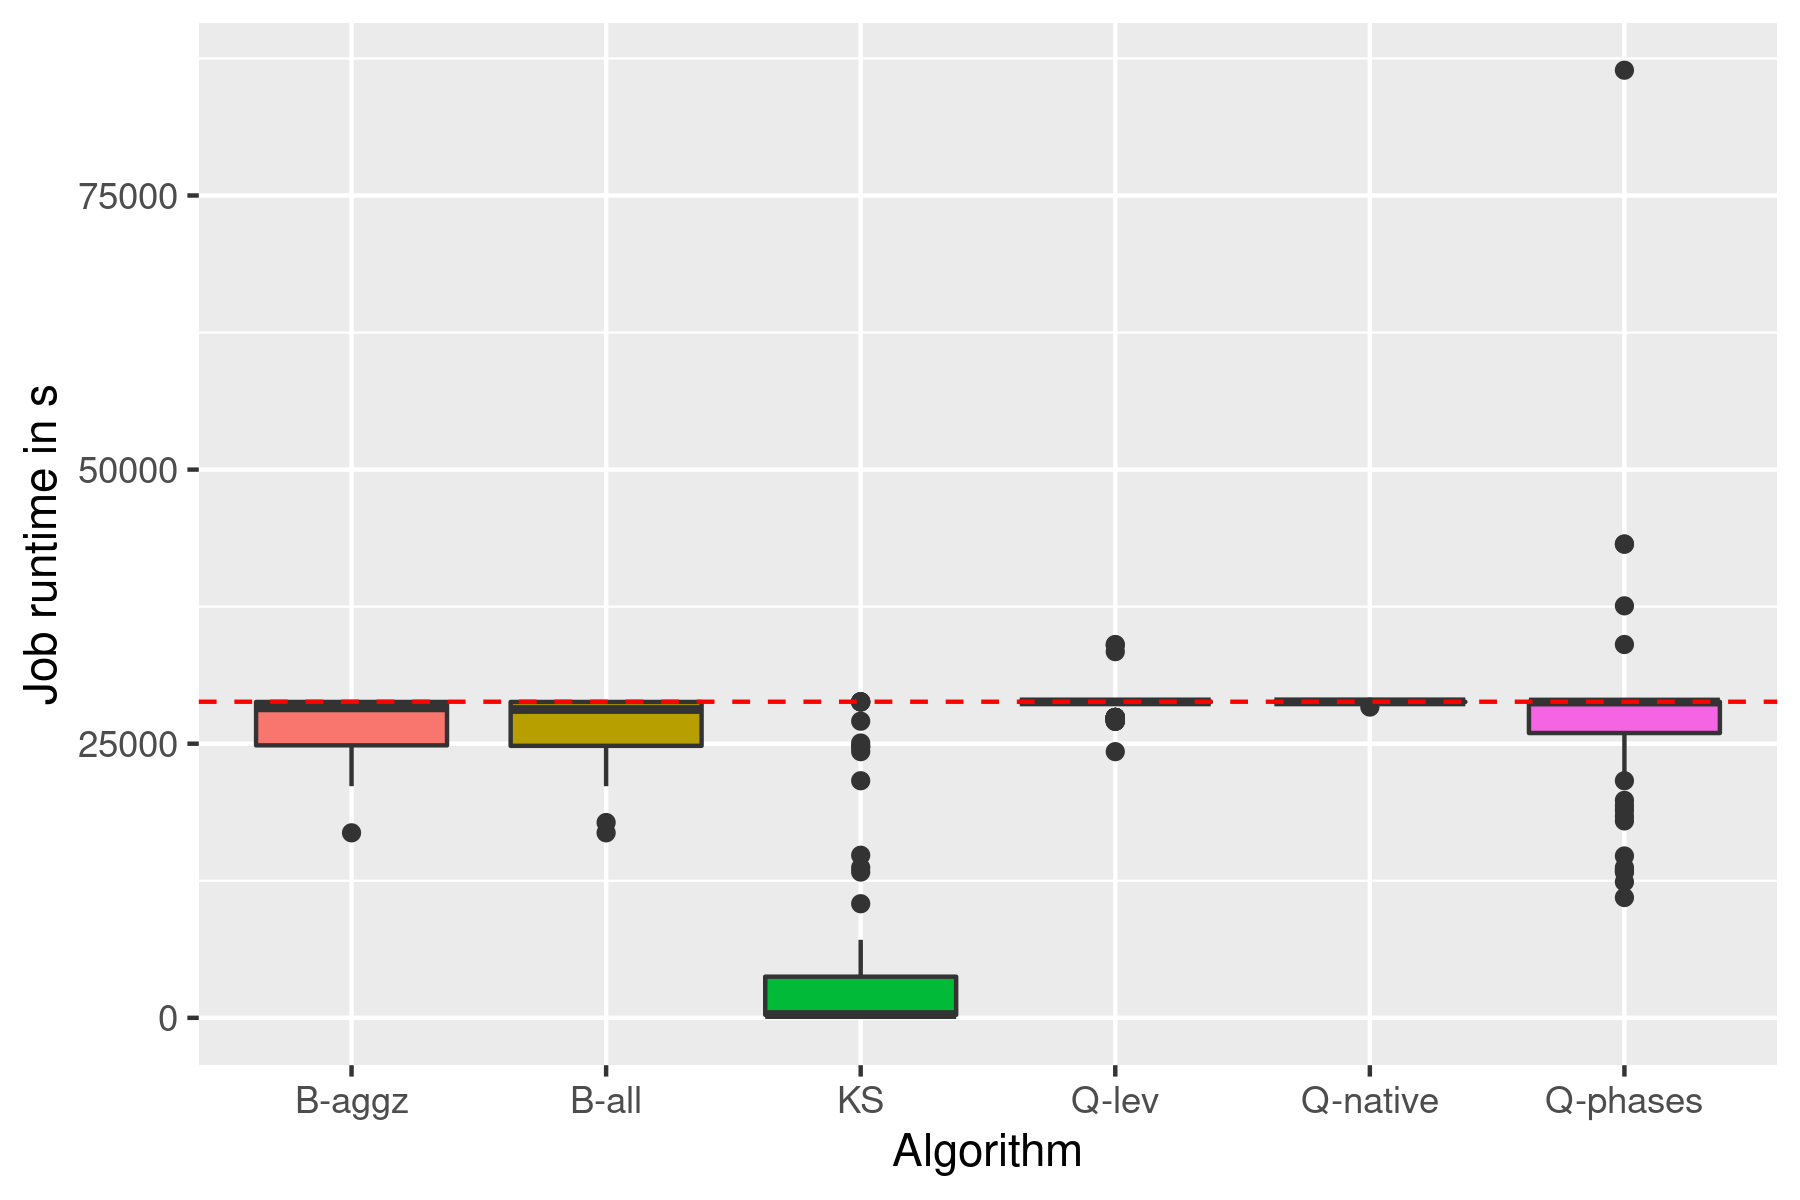
\includegraphics[width=\textwidth]{job_similarities_5024292-out/jobs-elapsed}
\caption{Job-M ($job=28,828s$)}\label{fig:runtime-job-M}
\end{subfigure}
\begin{subfigure}{0.7\textwidth}
\centering
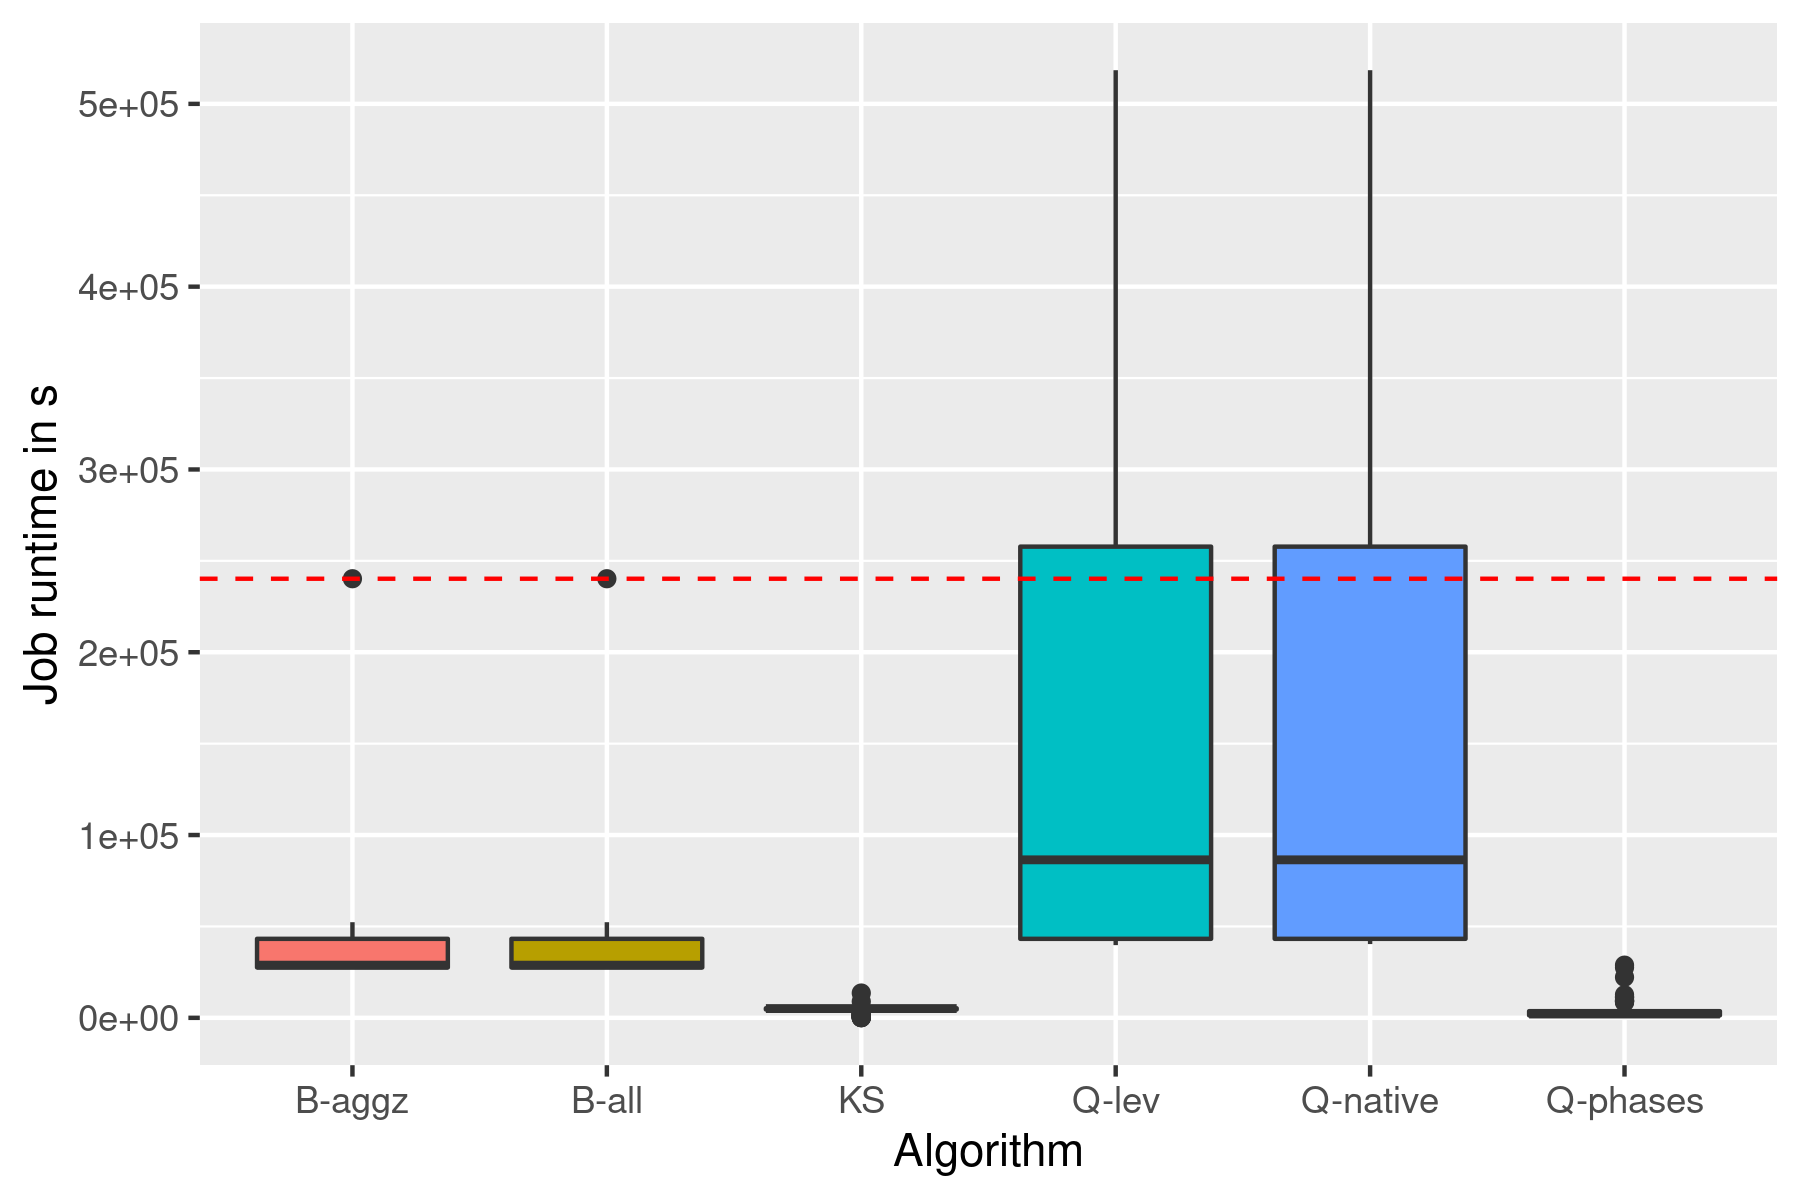
\includegraphics[width=\textwidth]{job_similarities_7488914-out/jobs-elapsed}
\caption{Job-L ($job=240ks$)}\label{fig:runtime-job-L}
\end{subfigure}
\centering
\caption{Distribution of runtime for all 100 top-ranked jobs}%
\label{fig:runtime-job}
\end{figure}

\subsubsection{Algorithmic differences}
To verify that the different algorithms behave differently, the intersection for the Top\,100 is computed for all combinations of algorithms and visualized in \Cref{fig:heatmap-job}.
B-all and B-aggz overlap with at least 99 ranks for all three jobs.
While there is some reordering, both algorithms lead to a comparable set.
All algorithms have a significant overlap for Job-S.
For Job-M, however, they lead to a different ranking, and Top\,100, particularly KS determines a different set.
Generally, Q-lev and Q-native are generating more similar results than other algorithms.
From this analysis, we conclude that one representative from B is sufficient as it generates very similar results while the other algorithms identify mostly disjoint behavioral aspects. % and, therefore, should be analyzed individually


\begin{figure}[t]
\begin{subfigure}{0.48\textwidth}
\centering
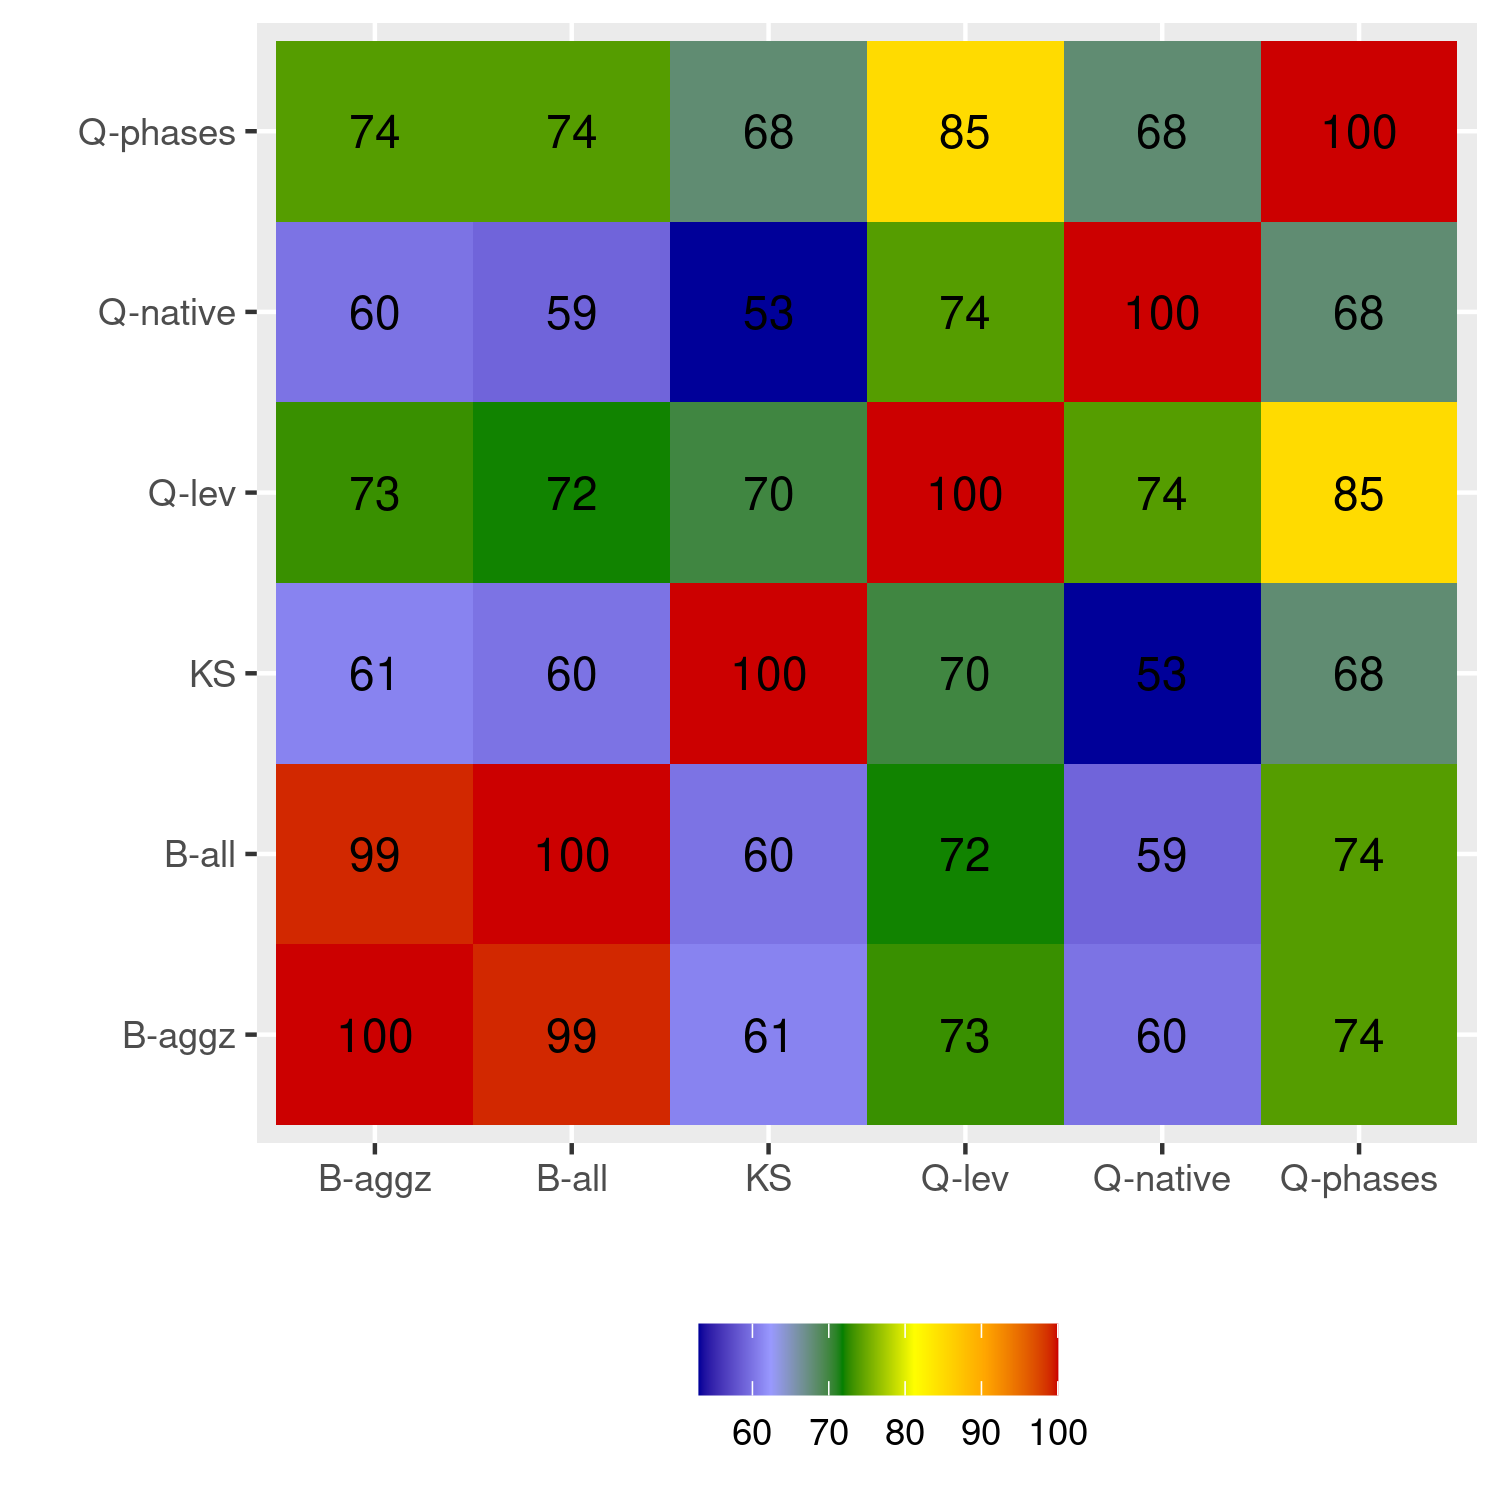
\includegraphics[width=\textwidth]{job_similarities_4296426-out/intersection-heatmap}
\caption{Job-S}\label{fig:heatmap-job-S}
\end{subfigure}
\begin{subfigure}{0.48\textwidth}
\centering
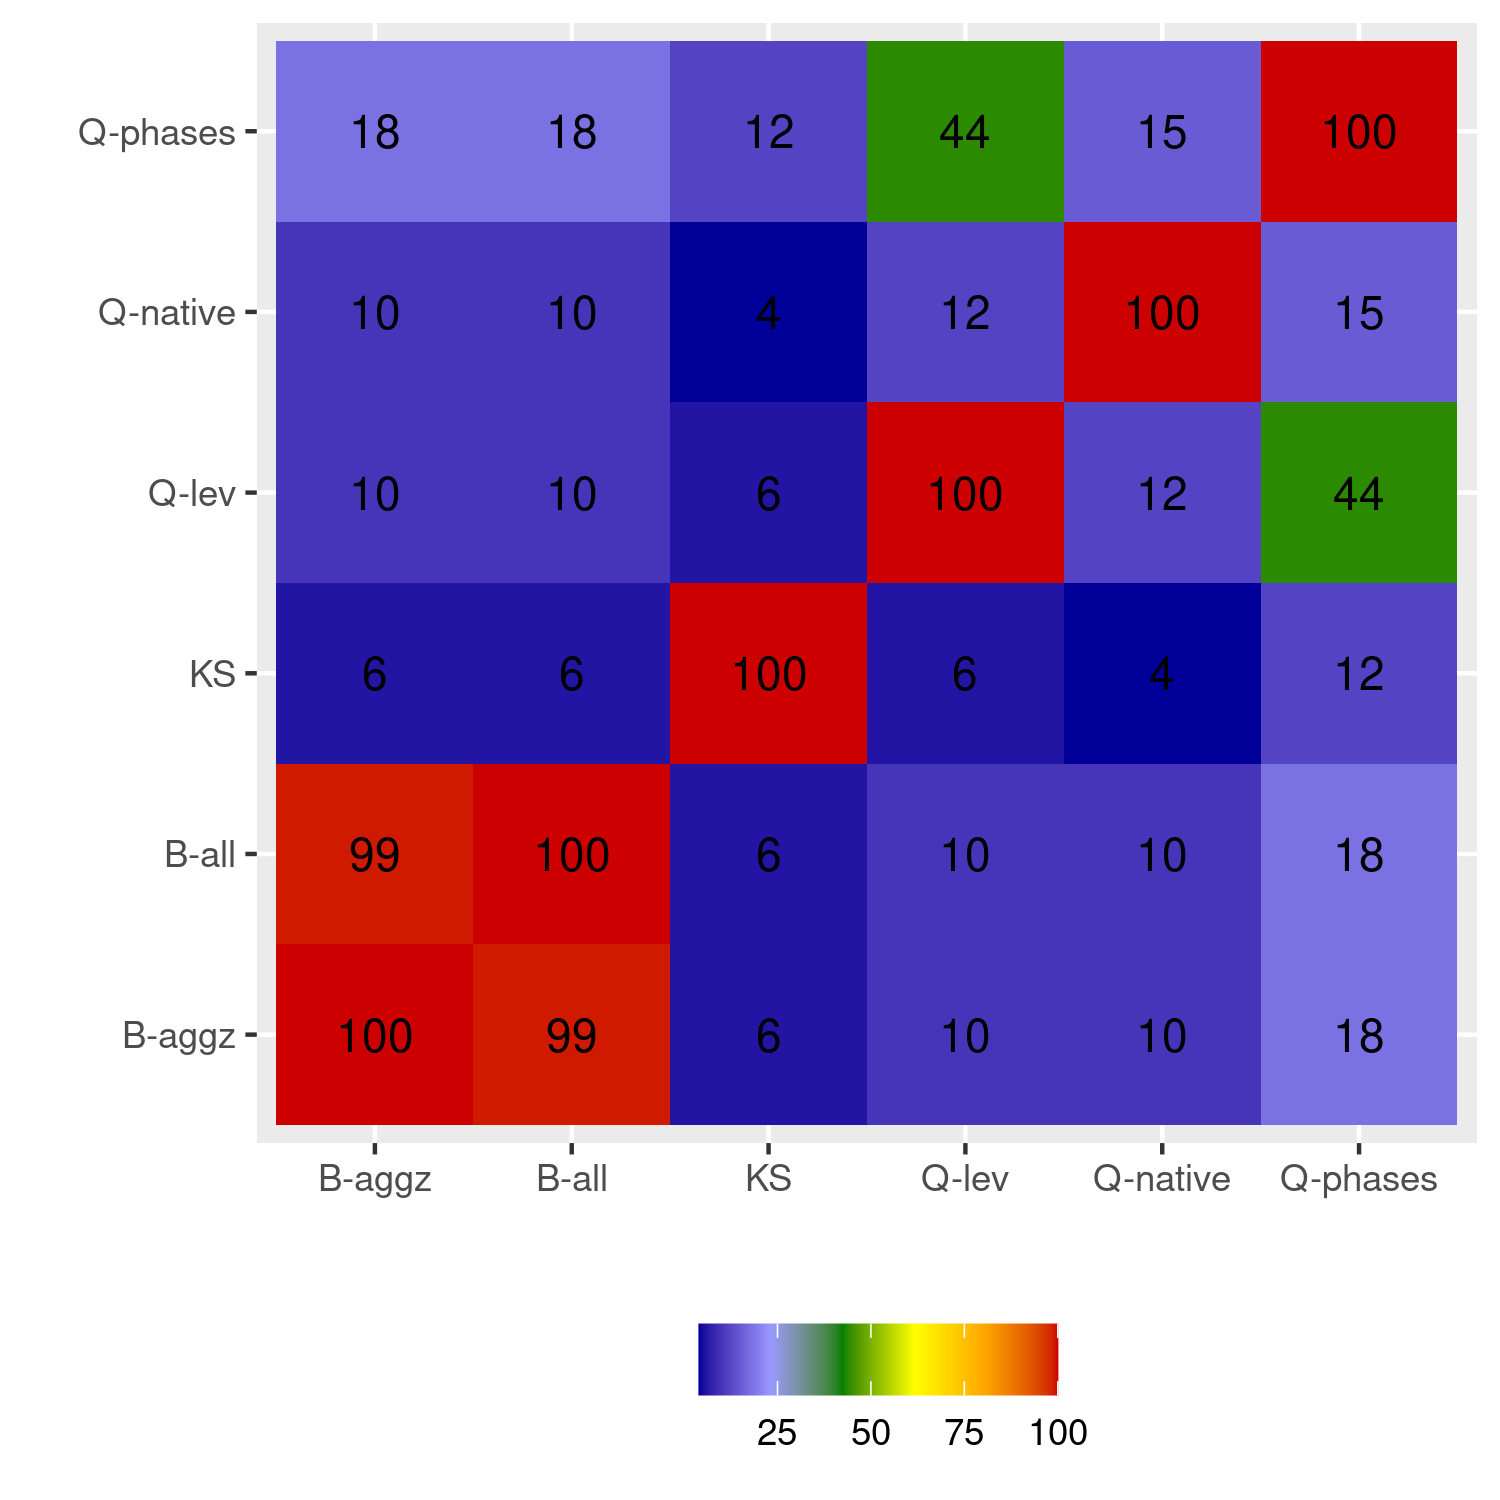
\includegraphics[width=\textwidth]{job_similarities_5024292-out/intersection-heatmap}
\caption{Job-M}\label{fig:heatmap-job-M} %,trim={2.5cm 0 0 0},clip
\end{subfigure}
\begin{subfigure}{0.52\textwidth}
\centering
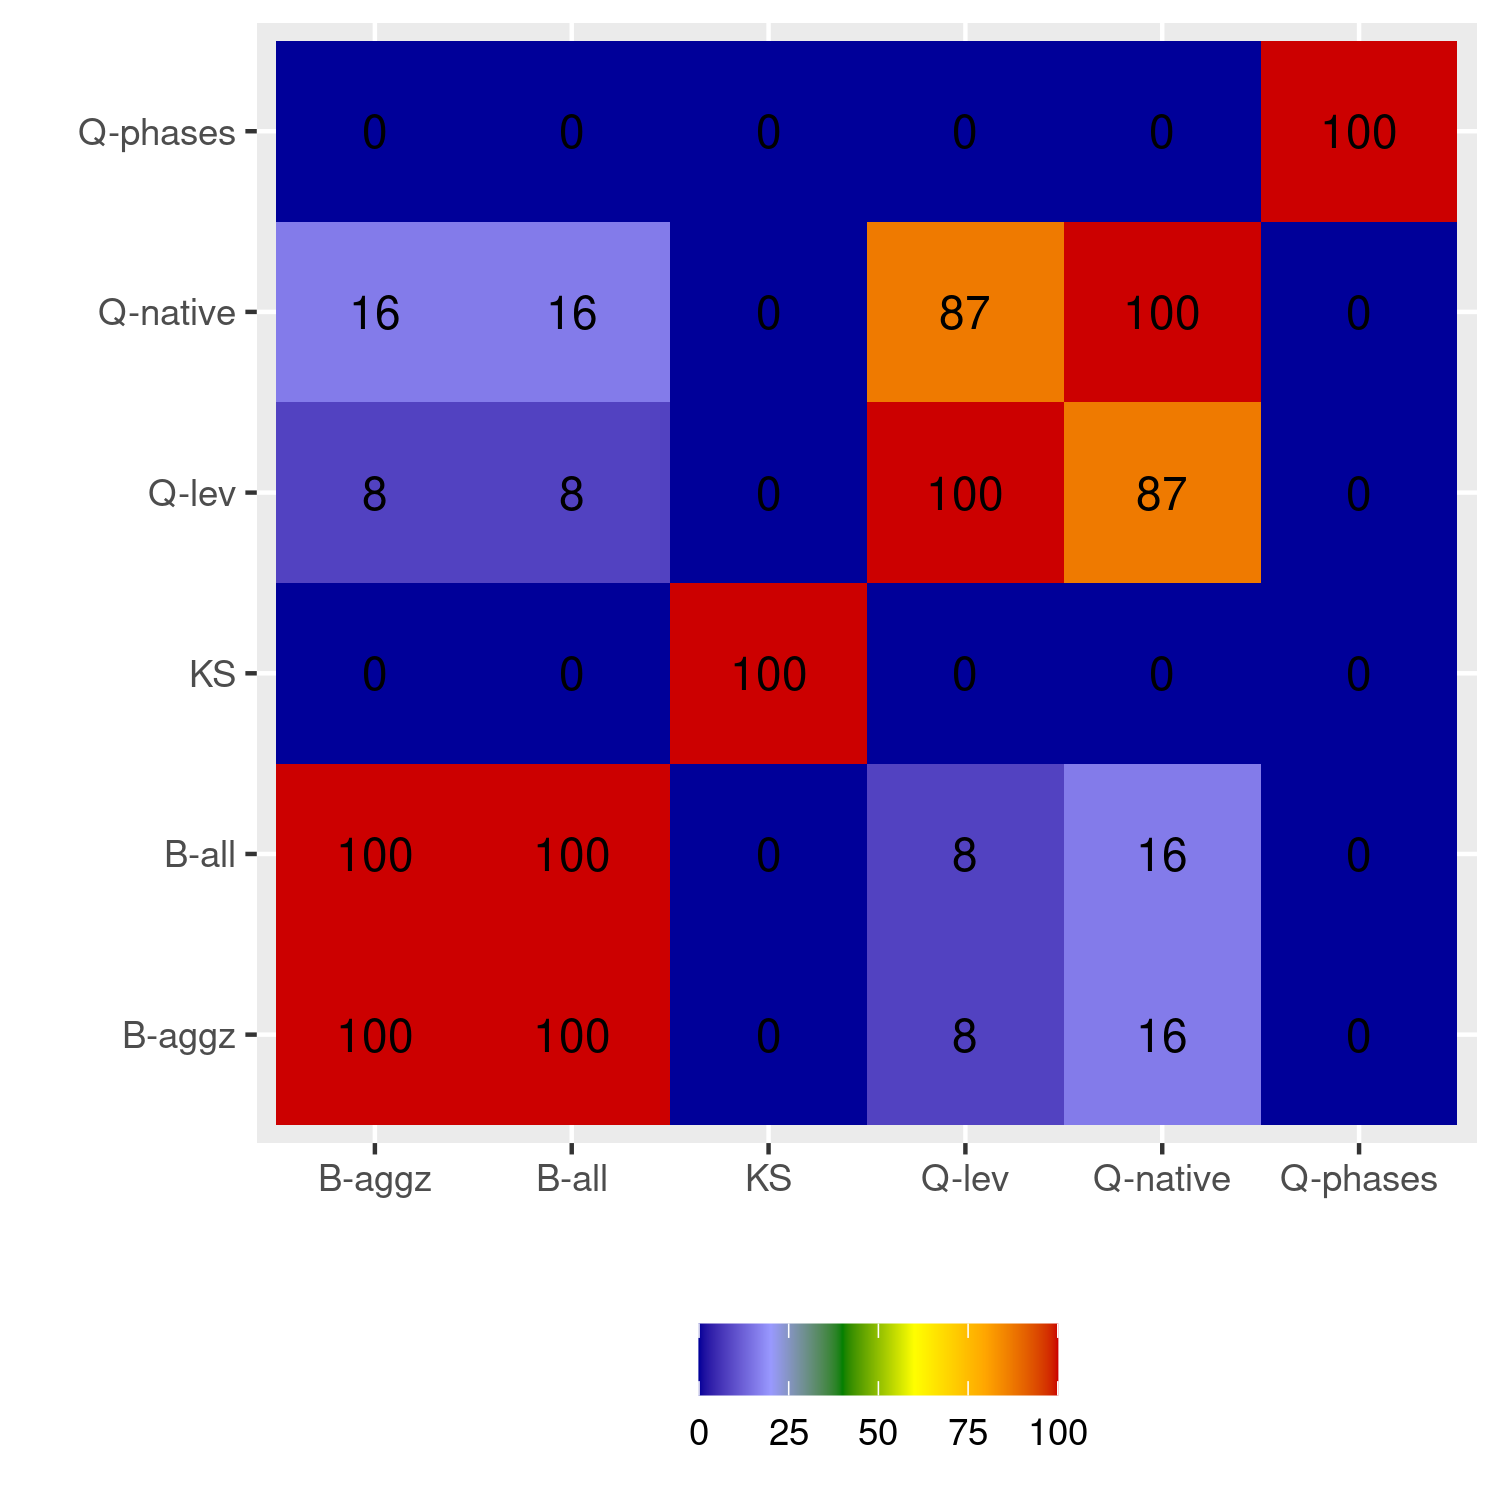
\includegraphics[width=\textwidth]{job_similarities_7488914-out/intersection-heatmap}
\caption{Job-L}\label{fig:heatmap-job-L}
\end{subfigure}

\centering
\caption{Intersection of the 100 top-ranked jobs for different algorithms}%
\label{fig:heatmap-job}
\end{figure}

%%%%%%%%%%% %%%%%%%%%%% %%%%%%%%%%% %%%%%%%%%%% %%%%%%%%%%% %%%%%%%%%%% %%%%%%%%%%% %%%%%%%%%%%

\section{Assessing Timelines for Similar Jobs}%
\label{sec:timelines}
To verify the suitability of the similarity metrics, for each algorithm, we carefully investigated the timelines of each of the jobs in the Top\,100.
We subjectively found that the approach works very well and identifies suitable similar jobs.
To demonstrate this, we include a selection of job timelines  and selected interesting job profiles.
These can be visually and subjectively compared to our reference jobs shown in \Cref{fig:refJobs}.
For space reasons, the included images will be scaled down making it difficult to read the text.
However, we believe that they are still well suited for a visual inspection and comparison.

\subsection{Job-S}

This job represents post-processing (CMORization) which is a typical step.
It is executed for different simulations and variables across timesteps.
The job name suggests that it is applied to the control variable.
In the metadata, we found 22,580 jobs with “cmor” in the name of which 367 jobs mention “control”.

The B and KS algorithms identify one job whose name doesn't include “cmor”.
All other algorithms identify only “cmor” jobs and 26-38 of these jobs are applied to “control” (see \Cref{tbl:control-jobs}) -- only the KS algorithm doesn't identify any job with control.
A selection of job timelines on control variables is given in \Cref{fig:job-S-hex-lev}.
The single non-cmor job and a high-ranked non-control cmor job is shown in \Cref{fig:job-S-bin-agg}.
While we cannot visually see many differences between these two jobs compared to the control job, the algorithms indicate that jobs processing the control variables are more similar as they are more frequent in the Top\,100 jobs.
For Job-S, we found that all algorithms work well and, therefore, omit further timelines.

\begin{table}[bt]
\centering
\begin{tabular}{r|r|r|r|r|r}
  B-aggz & B-all & Q-lev & Q-native & Q-phases & KS\\ \hline
  38 &   38 &   33 &   26 &   33 &       0
\end{tabular}

  \caption{Job-S: number of jobs with “control” in their name in the Top-100}%
  \label{tbl:control-jobs}
\end{table}

\begin{figure}[bt]
\centering
\begin{subfigure}{0.47\textwidth}
\centering
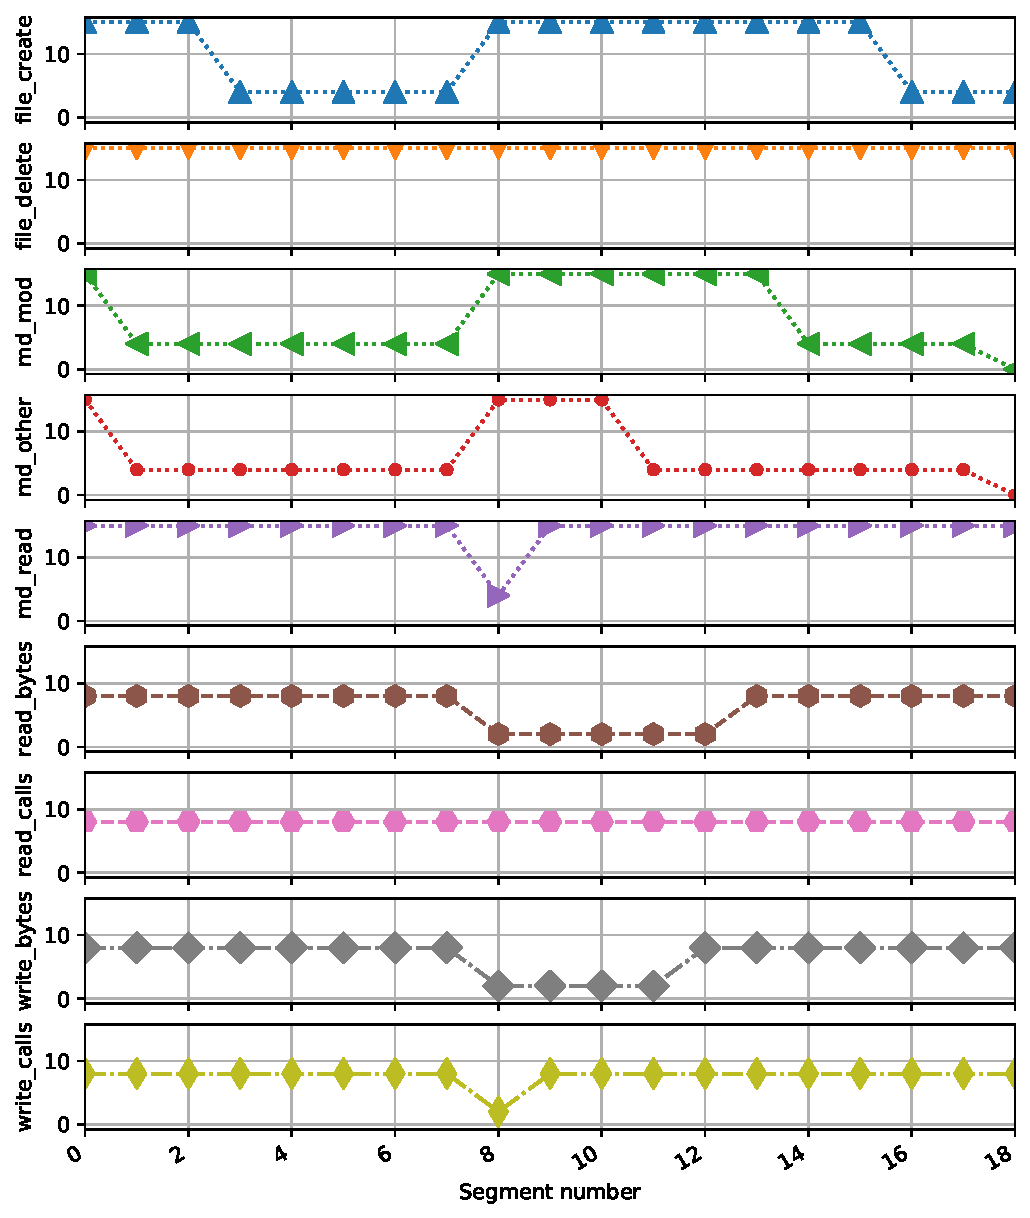
\includegraphics[width=\textwidth]{job_similarities_4296426-out/bin_aggzeros-0.6923--76timeseries4235560}
\caption{Non-cmor job: Rank\,76, SIM=69\%}
\end{subfigure}
\qquad
\begin{subfigure}{0.47\textwidth}
\centering
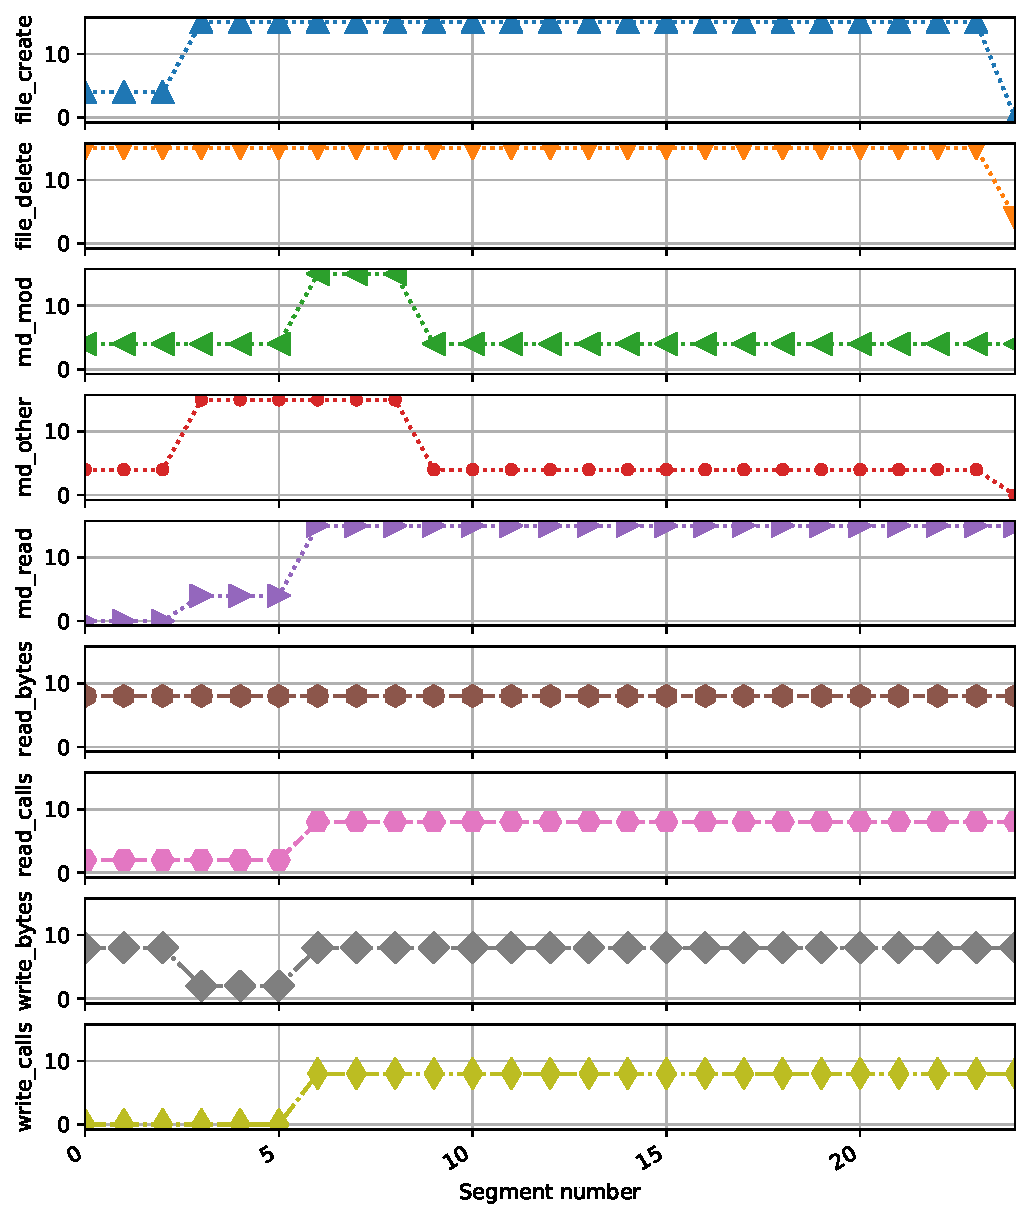
\includegraphics[width=\textwidth]{job_similarities_4296426-out/bin_aggzeros-0.8077--4timeseries4483904}
\caption{Non-control job: Rank\,4, SIM=81\%}
\end{subfigure}

\caption{Job-S: jobs with different job names when using B-aggz}%
\label{fig:job-S-bin-agg}
\end{figure}


\begin{figure}[bt]
\begin{subfigure}{0.47\textwidth}
\centering
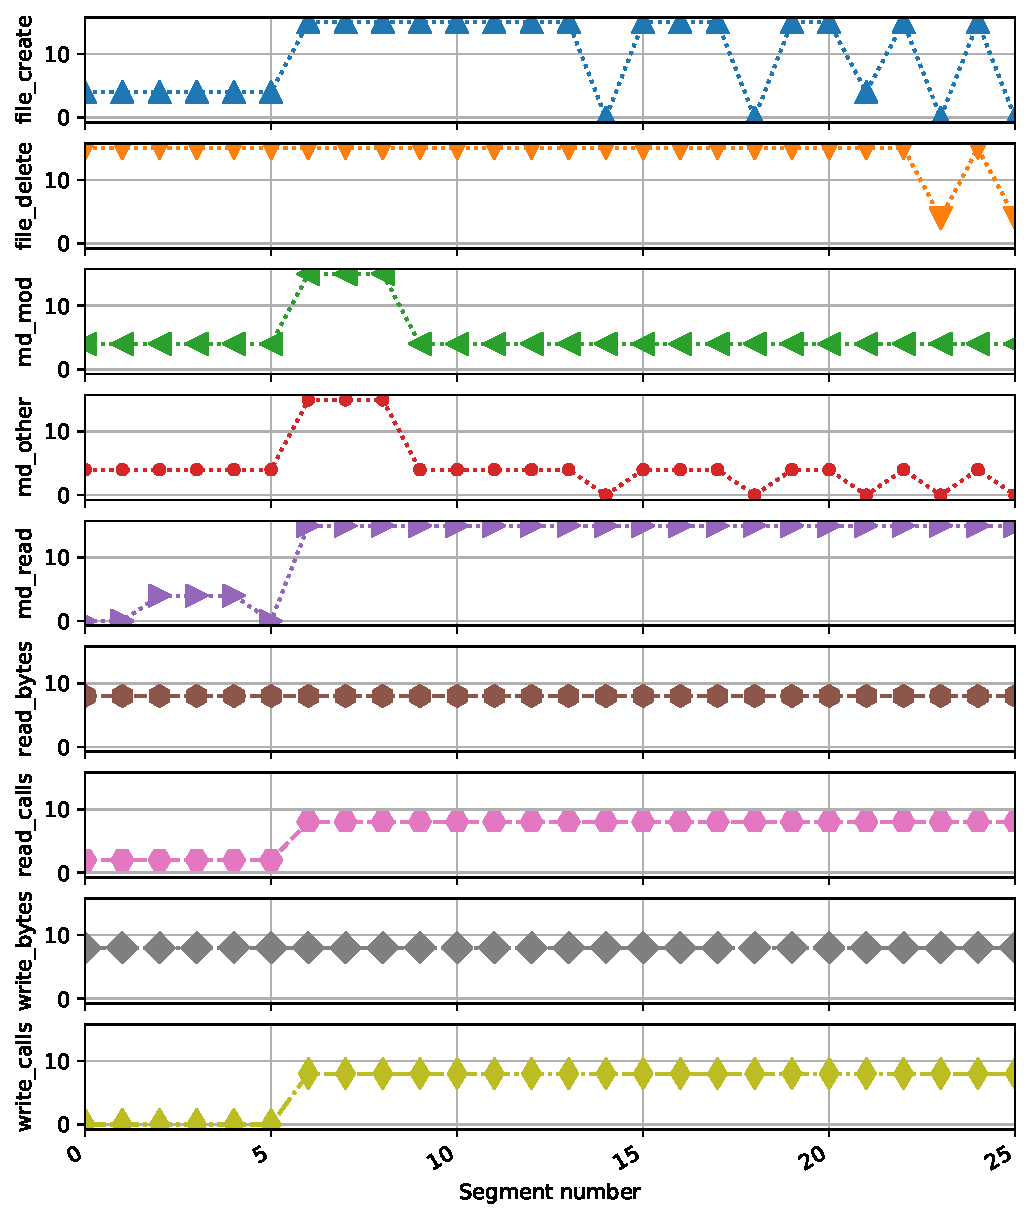
\includegraphics[width=\textwidth]{job_similarities_4296426-out/hex_lev-0.9615--1timeseries4296288}
\caption{Rank 2, SIM=96\%}
\end{subfigure}
\begin{subfigure}{0.47\textwidth}
\centering
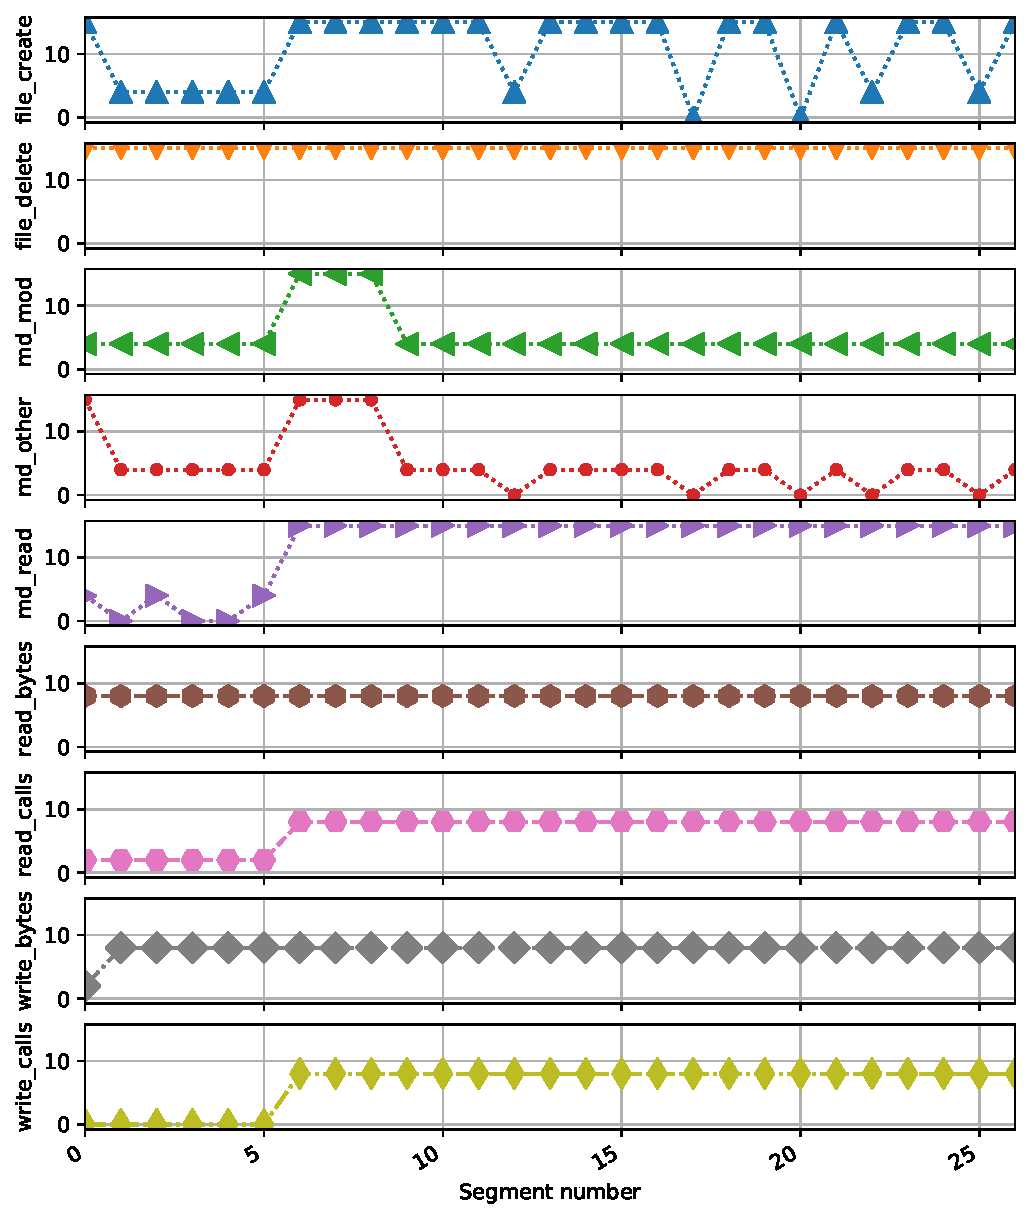
\includegraphics[width=\textwidth]{job_similarities_4296426-out/hex_lev-0.9012--15timeseries4296277}
\caption{Rank 15, SIM=90\%}
\end{subfigure}
\begin{subfigure}{0.47\textwidth}
\centering
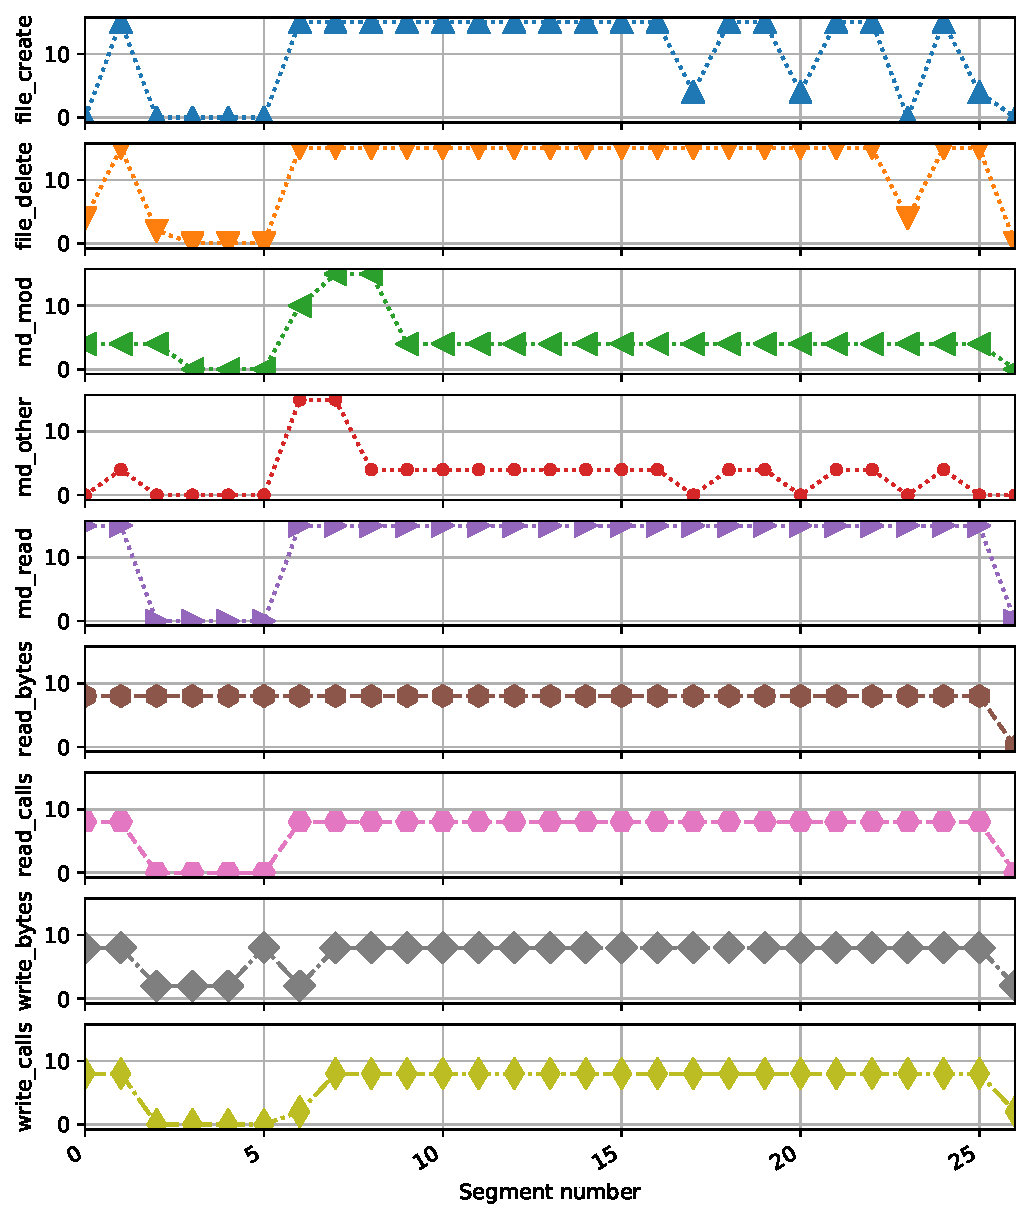
\includegraphics[width=\textwidth]{job_similarities_4296426-out/hex_lev-0.7901--99timeseries4297842}
\caption{Rank\,100, SIM=79\%}
\end{subfigure}

\caption{Job-S with Q-Lev, selection of similar jobs}%
\label{fig:job-S-hex-lev}
\end{figure}

% \begin{figure}
% \begin{subfigure}{0.3\textwidth}
% \centering
% \includegraphics[width=\textwidth]{job_similarities_4296426-out/hex_native-0.9808--1timeseries4296288}
% \caption{Rank 2, SIM=}
% \end{subfigure}
% \begin{subfigure}{0.3\textwidth}
% \centering
% \includegraphics[width=\textwidth]{job_similarities_4296426-out/hex_native-0.9375--15timeseries4564296}
% \caption{Rank 15, SIM=}
% \end{subfigure}
% \begin{subfigure}{0.3\textwidth}
% \centering
% \includegraphics[width=\textwidth]{job_similarities_4296426-out/hex_native-0.8915--99timeseries4296785}
% \caption{Rank\,100, SIM=}
% \end{subfigure}
% \caption{Job-S with Hex-Native, selection of similar jobs}
% \label{fig:job-S-hex-native}
% \end{figure}
%
% \ContinuedFloat

%
% \begin{figure}
% \begin{subfigure}{0.3\textwidth}
% \centering
% \includegraphics[width=\textwidth]{job_similarities_4296426-out/bin_aggzeros-0.8462--1timeseries4296280}
% \caption{Rank 2, SIM=}
% \end{subfigure}
% \begin{subfigure}{0.3\textwidth}
% \centering
% \includegraphics[width=\textwidth]{job_similarities_4296426-out/bin_aggzeros-0.7778--14timeseries4555405}
% \caption{Rank 15, SIM=}
% \end{subfigure}
% \begin{subfigure}{0.3\textwidth}
% \centering
% \includegraphics[width=\textwidth]{job_similarities_4296426-out/bin_aggzeros-0.6923--99timeseries4687419}
% \caption{Rank\,100, SIM=}
% \end{subfigure}
% \caption{Job-S with B-aggzero, selection of similar jobs}
% \label{fig:job-S-bin-aggzeros}
% \end{figure}


\subsection{Job-M}

Inspecting the Top\,100 for this reference job is highlighting the differences between the algorithms.
All algorithms identify a diverse range of job names for this reference job in the Top\,100.
Firstly, the same name of the reference job appears 30 times in the whole dataset. 
Additional 932 jobs have a slightly modified name.
So this job type isn't necessarily executed frequently and, therefore, our Top\,100 is expected to contain other names.
All algorithms identify only the reference job but none of the other jobs with the identical name but 1 (KS), 2 (B-* and Q-native) to 3 (Q-lev and Q-phases) jobs with slightly modified names.
Some applications are more prominent in these sets, e.g., for B-aggzero, 32~jobs contain WRF (a model) in the name.
The number of unique names is 19, 38, 49, and 51 for B-aggzero, Q-phases, Q-native and Q-lev, respectively.

When inspecting their timelines, the jobs that are similar according to the B algorithms (see \Cref{fig:job-M-bin-aggzero}) subjectively appear to us to be different. 
The reason lies in the definition of the B-* similarity which aggregate all I/O statistics into one timeline.
The other algorithms like Q-lev (\Cref{fig:job-M-hex-lev}) and Q-native (\Cref{fig:job-M-hex-native}) seem to work as intended:
While jobs exhibit short bursts of other active metrics even for low similarity, we can eyeball a relevant similarity particularly for Rank\,2 and Rank\,3 which have the high similarity of 90+\%. For Rank\,15 to Rank\,100, with around 70\% similarity, a partial match of the metrics is still given.
The KS algorithm working on the histograms ranks the jobs correctly on the similarity of their histograms.
However, as it does not deal with the length of the jobs, it may identify jobs of very different length.
In \Cref{fig:job-M-ks}, we see the 3rd ranked job whose profile is indeed quite similar but the time series differs but it is just running for 10min (1 segment) on 10\,nodes.
Remember, for the KS algorithm, we concatenate the metrics of all nodes together instead of averaging it in order to explore if node-specific information helps the similarity.

\begin{figure}[bt]
\begin{subfigure}{0.5\textwidth}
\centering
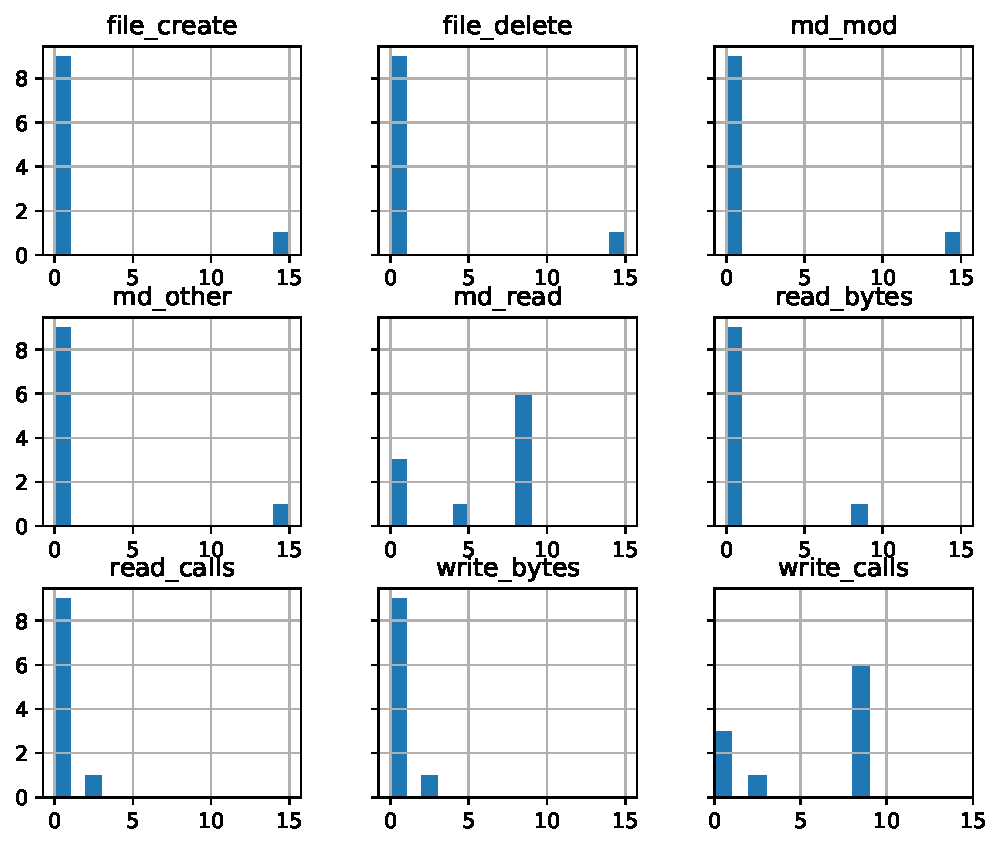
\includegraphics[width=\textwidth]{job_similarities_5024292-out/ks-0.7863--ks-2hist7827264}
\caption{Histogram}
\end{subfigure}
\qquad
\begin{subfigure}{0.36\textwidth}
\centering
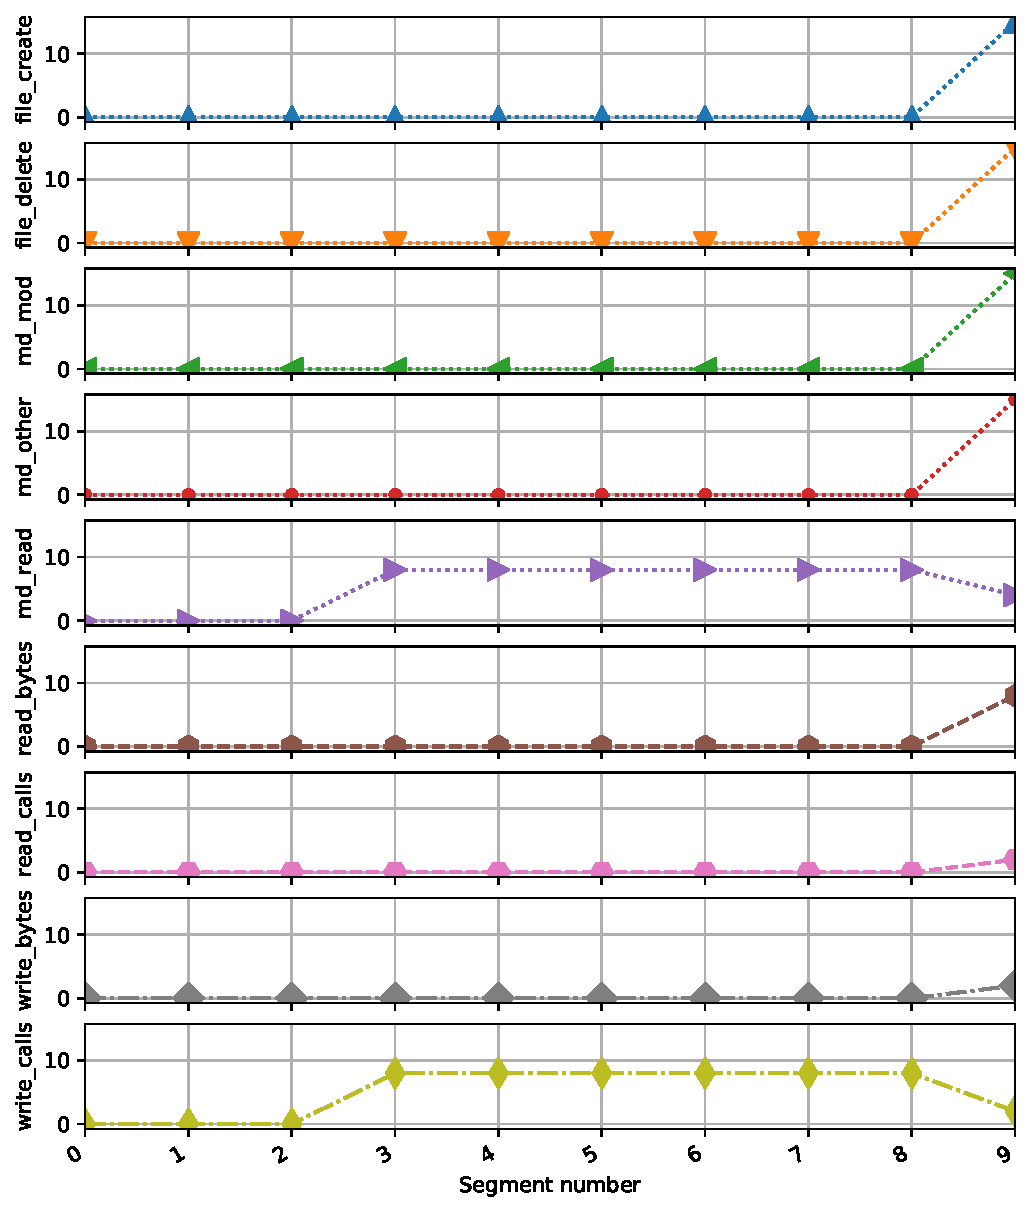
\includegraphics[width=\textwidth]{job_similarities_5024292-out/ks-0.7863--ks-2timeseries7827264}
\caption{Concatenated time series}
\end{subfigure}

\caption{Job-M with KS, for Rank\,3, SIM=78\%}%
\label{fig:job-M-ks}
\end{figure}




\begin{figure}[bt]
\begin{subfigure}{0.47\textwidth}
\centering
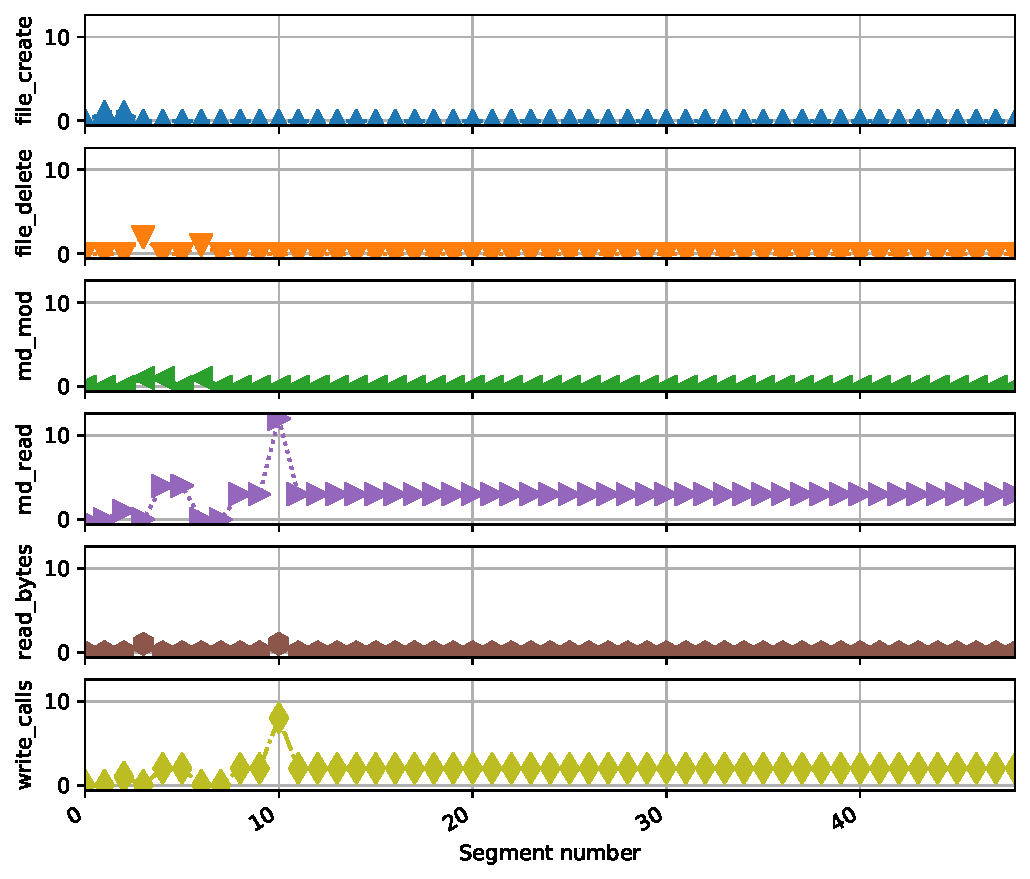
\includegraphics[width=\textwidth]{job_similarities_5024292-out/bin_aggzeros-0.7347--14timeseries4498983}
\caption{Rank\,15, SIM=73\%}
\end{subfigure}
\begin{subfigure}{0.47\textwidth}
\centering
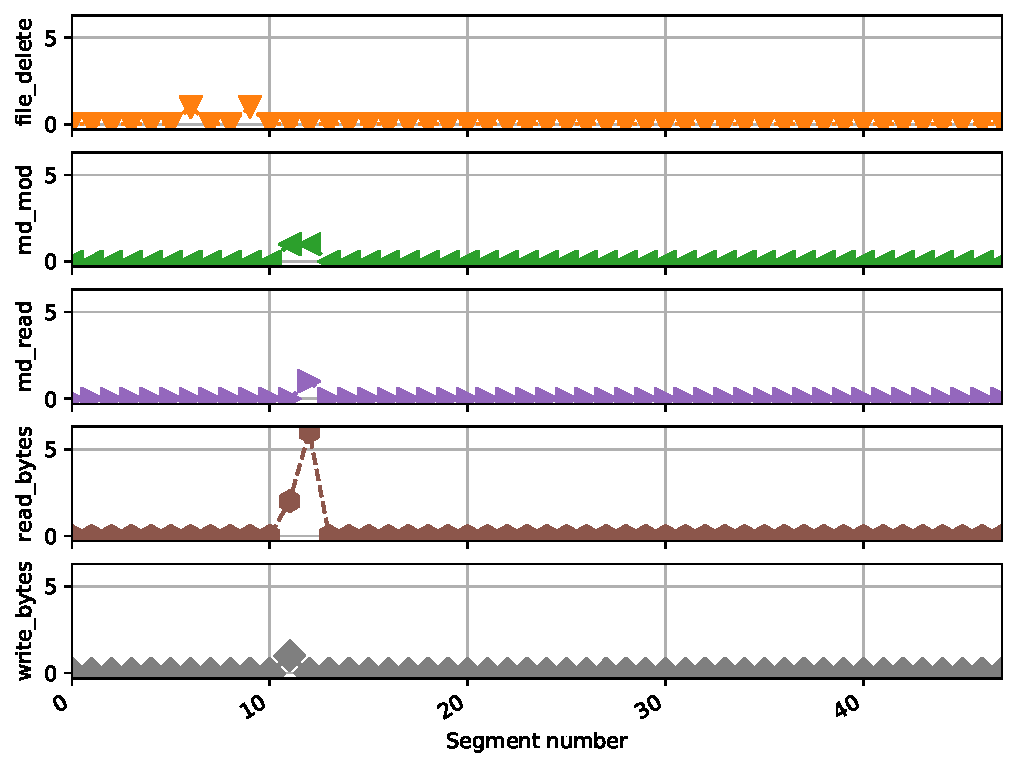
\includegraphics[width=\textwidth]{job_similarities_5024292-out/bin_aggzeros-0.5102--99timeseries5120077}
\caption{Rank\,100, SIM=51\% }
\end{subfigure}

\begin{subfigure}{0.47\textwidth}
\centering
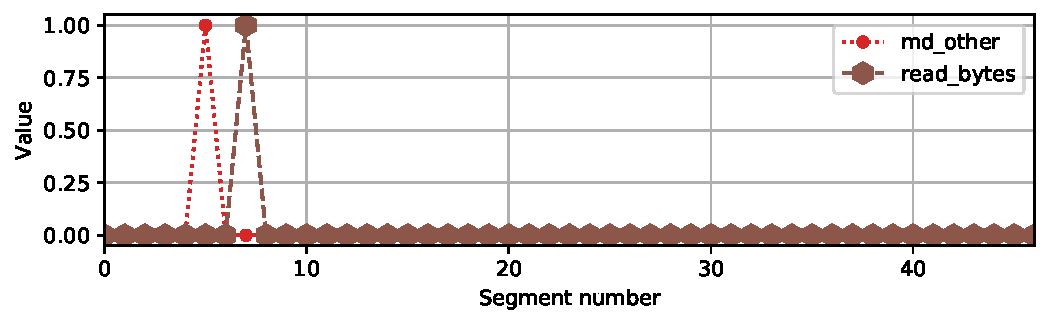
\includegraphics[width=\textwidth]{job_similarities_5024292-out/bin_aggzeros-0.7755--1timeseries8010306}
\caption{Rank\,2, SIM=78\%}
\end{subfigure}
\caption{Job-M with Bin-Aggzero, selection of similar jobs}%
\label{fig:job-M-bin-aggzero}
\end{figure}



\begin{figure}[bt]
\begin{subfigure}{0.47\textwidth}
\centering
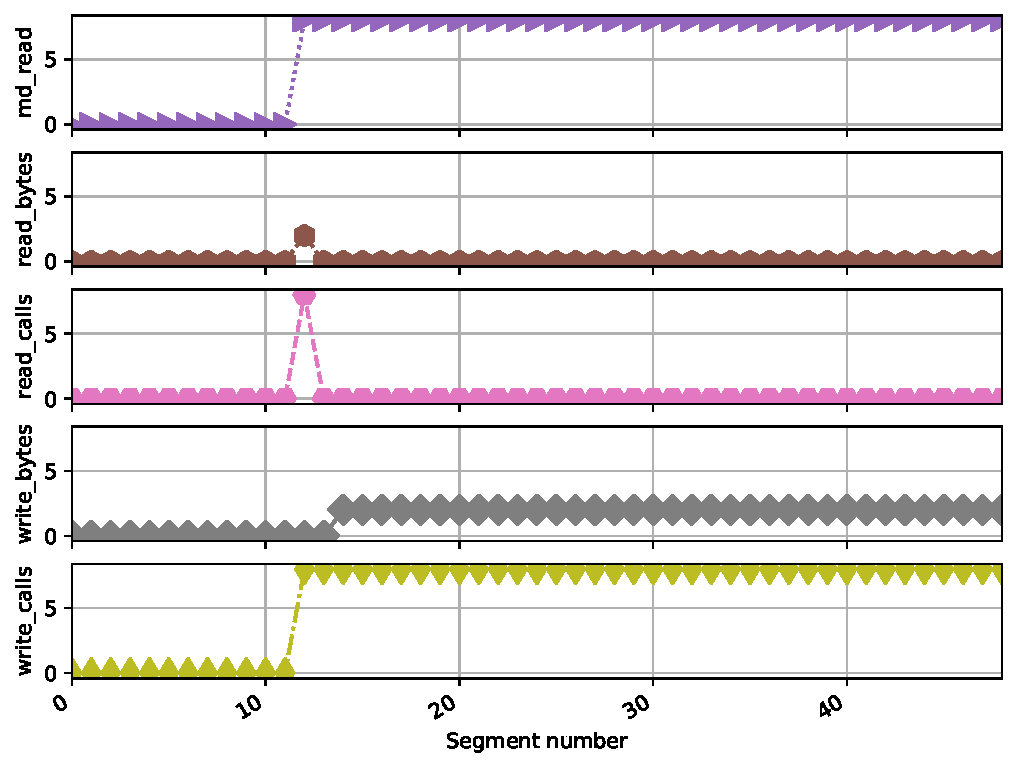
\includegraphics[width=\textwidth]{job_similarities_5024292-out/hex_lev-0.9365--2timeseries5240733}
\caption{Rank 3, SIM=94\%}
\end{subfigure}
\begin{subfigure}{0.47\textwidth}
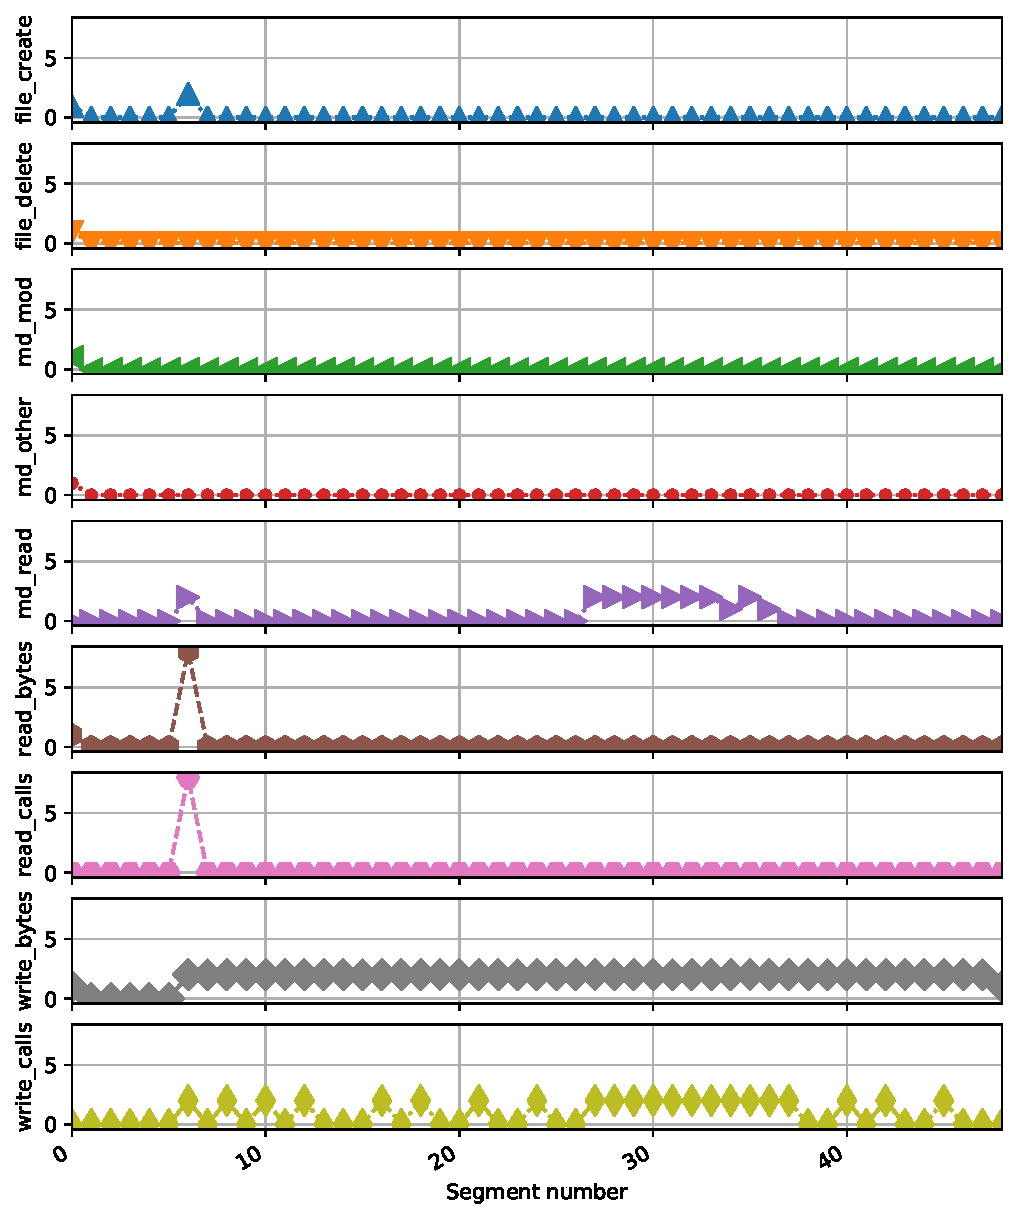
\includegraphics[width=\textwidth]{job_similarities_5024292-out/hex_lev-0.7392--15timeseries7651420}
\caption{Rank\,15, SIM=74\%}
\end{subfigure}

\begin{subfigure}{0.47\textwidth}
\centering
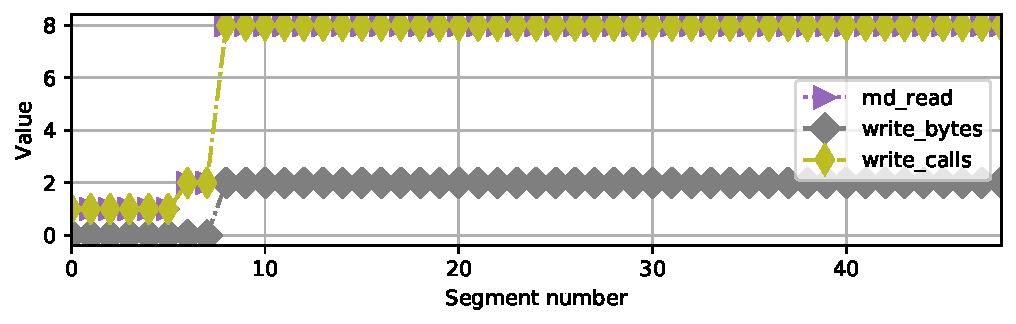
\includegraphics[width=\textwidth]{job_similarities_5024292-out/hex_lev-0.9546--1timeseries7826634}
\caption{Rank\,2, SIM=95\%}
\end{subfigure}
\begin{subfigure}{0.47\textwidth}
\centering
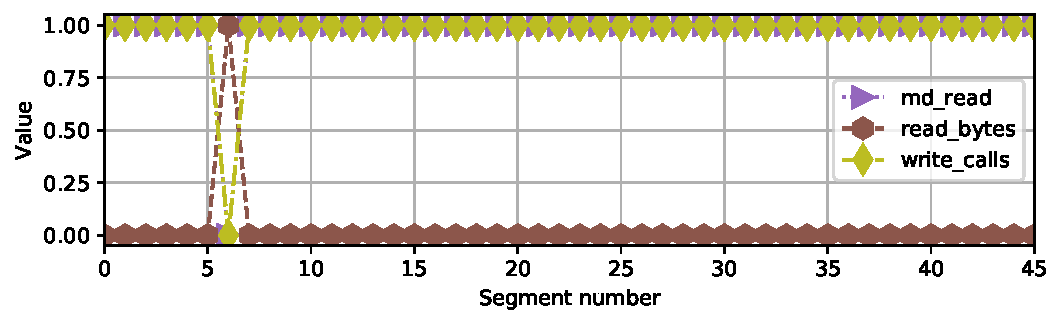
\includegraphics[width=\textwidth]{job_similarities_5024292-out/hex_lev-0.7007--99timeseries8201967}
\caption{Rank\,100, SIM=70\%}
\end{subfigure}

\caption{Job-M with Q-lev, selection of similar jobs}%
\label{fig:job-M-hex-lev}
\end{figure}



\begin{figure}[bt]
\begin{subfigure}{0.47\textwidth}
\centering
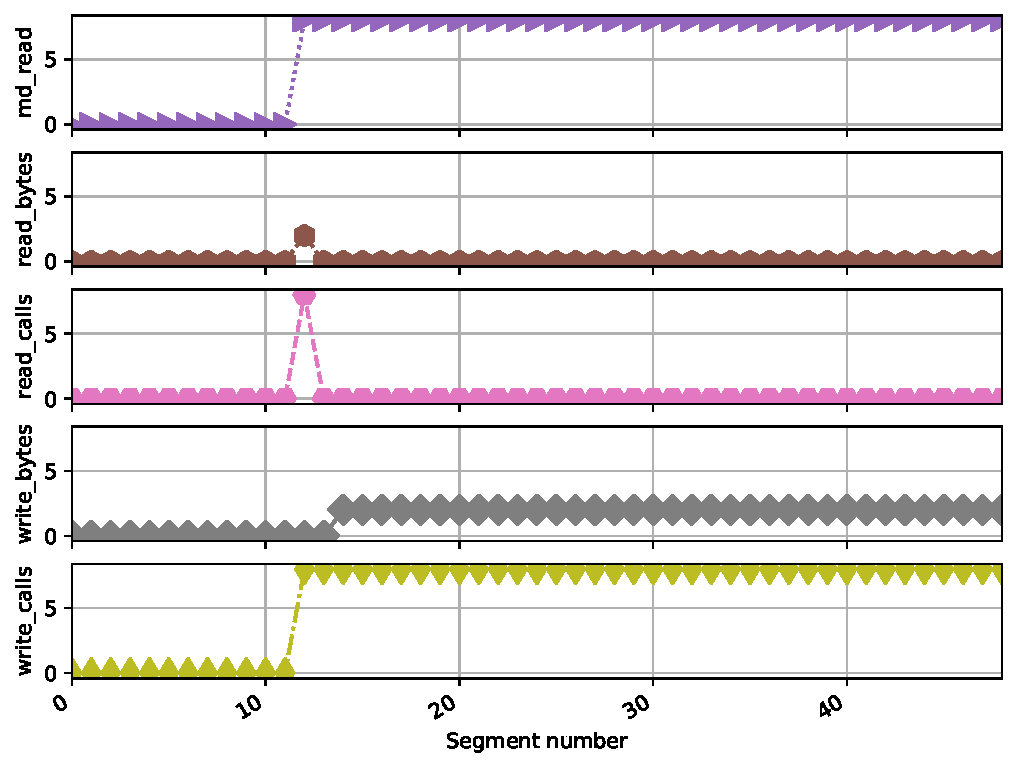
\includegraphics[width=\textwidth]{job_similarities_5024292-out/hex_native-0.9878--1timeseries5240733}
\caption{Rank 2, SIM=99\%}
\end{subfigure}
\begin{subfigure}{0.47\textwidth}
\centering
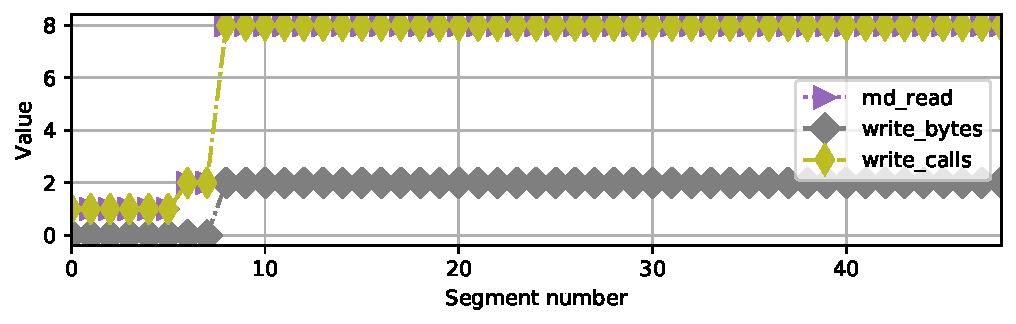
\includegraphics[width=\textwidth]{job_similarities_5024292-out/hex_native-0.9651--2timeseries7826634}
\caption{Rank 3, SIM=97\%}
\end{subfigure}
\begin{subfigure}{0.47\textwidth}
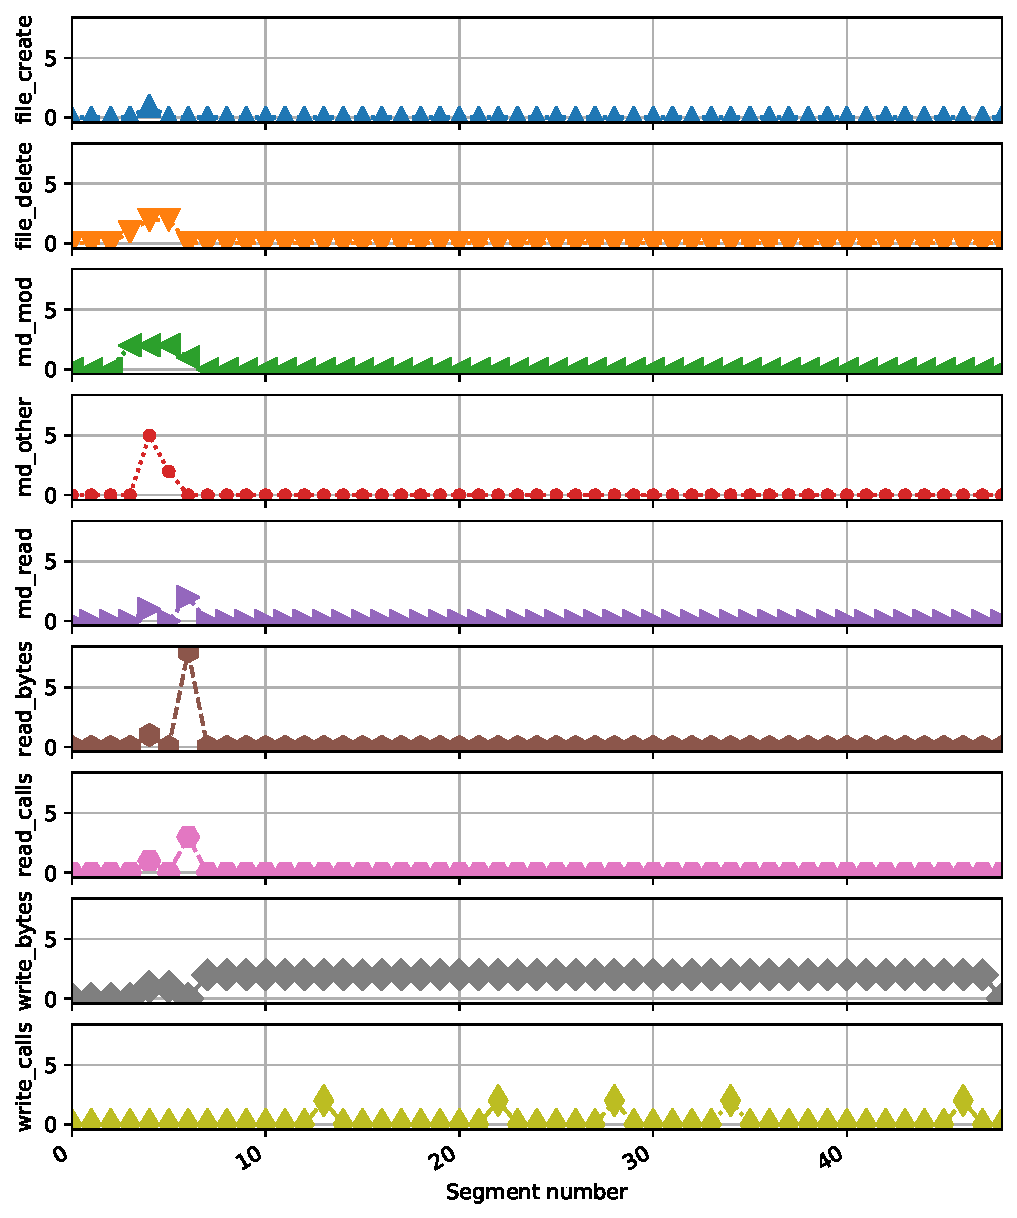
\includegraphics[width=\textwidth]{job_similarities_5024292-out/hex_native-0.9084--14timeseries8037817}
\caption{Rank 15, SIM=91\%}
\end{subfigure}
\begin{subfigure}{0.47\textwidth}
\centering
\includegraphics[width=\textwidth]{job_similarities_5024292-out/hex_native-0.8838--99timeseries7571967}
\caption{Rank 100, SIM=88\%}
\end{subfigure}

\caption{Job-M with Q-native, selection of similar jobs}%
\label{fig:job-M-hex-native}
\end{figure}

%
% \begin{figure}[bt]
% \begin{subfigure}{0.3\textwidth}
% \centering
% \includegraphics[width=\textwidth]{job_similarities_5024292-out/hex_phases-0.8831--1timeseries7826634}
% \caption{Rank 2, SIM=88\%}
% \end{subfigure}
% \begin{subfigure}{0.3\textwidth}
% \centering
% \includegraphics[width=\textwidth]{job_similarities_5024292-out/hex_phases-0.7963--2timeseries5240733}
% \caption{Rank 3, SIM=80\%}
% \end{subfigure}
% \begin{subfigure}{0.3\textwidth}
% \includegraphics[width=\textwidth]{job_similarities_5024292-out/hex_phases-0.4583--14timeseries4244400}
% \caption{Rank 15, SIM=46\%}
% \end{subfigure}
% \begin{subfigure}{0.3\textwidth}
% \centering
% \includegraphics[width=\textwidth]{job_similarities_5024292-out/hex_phases-0.2397--99timeseries7644009}
% \caption{Rank 100, SIM=24\%}
% \end{subfigure}
%
% \caption{Job-M with Q-phases, selection of similar jobs}
% \label{fig:job-M-hex-phases}
% \end{figure}

\subsection{Job-L}

The B algorithms find a low similarity (the best 2nd ranked job is 17\% similar), the inspection of job names (14 unique names) leads to two prominent applications: bash and xmessy with 45 and 48 instances, respectively.
In \Cref{fig:job-L-bin-aggzero}, it can be seen that the found jobs have little in common with the reference job.

The Q-lev and Q-native algorithms identify a more diverse set of applications (18 unique names and no xmessy job).
Q-native \Cref{fig:job-L-hex-native} finds long jobs with only little activity which, therefore, is similar to our reference job.
The Q-phases algorithm finds 85 unique names but as there is only one short I/O phase in the reference job, it finds many (short) jobs with 100\% similarity as seen in \Cref{fig:job-L-hex-phases}.
The KS algorithm is even more inclusive having 1285 jobs with 100\% similarity; the 100 selected ones contain 71 jobs ending with t127, which is a typical model configuration.
As expected, the histograms mimic the profile of the reference job, and thus, the algorithm does what it is expected to do.


\begin{figure}[bt]
\begin{subfigure}{0.47\textwidth}
\centering
\includegraphics[width=\textwidth]{job_similarities_7488914-out/bin_aggzeros-0.1671--1timeseries7869050}
\caption{Rank 2, SIM=17\%}
\end{subfigure}
\begin{subfigure}{0.47\textwidth}
\centering
\includegraphics[width=\textwidth]{job_similarities_7488914-out/bin_aggzeros-0.1671--2timeseries7990497}
\caption{Rank 3, SIM=17\%}
\end{subfigure}
\begin{subfigure}{0.47\textwidth}
\includegraphics[width=\textwidth]{job_similarities_7488914-out/bin_aggzeros-0.1521--14timeseries8363584}
\caption{Rank 15, SIM=15\%}
\end{subfigure}
\begin{subfigure}{0.47\textwidth}
\centering
\includegraphics[width=\textwidth]{job_similarities_7488914-out/bin_aggzeros-0.1097--97timeseries4262983}
\caption{Rank 100, SIM=11\%}
\end{subfigure}

\caption{Job-L with B-aggzero, selection of similar jobs}%
\label{fig:job-L-bin-aggzero}
\end{figure}

%
% \begin{figure}[bt]
% \begin{subfigure}{0.3\textwidth}
% \centering
% \includegraphics[width=\textwidth]{job_similarities_7488914-out/hex_lev-0.9386--1timeseries7266845}
% \caption{Rank 2, SIM=94\%}
% \end{subfigure}
% \begin{subfigure}{0.3\textwidth}
% \centering
% \includegraphics[width=\textwidth]{job_similarities_7488914-out/hex_lev-0.9375--2timeseries7214657}
% \caption{Rank 3, SIM=94\%}
% \end{subfigure}
% \begin{subfigure}{0.3\textwidth}
% \includegraphics[width=\textwidth]{job_similarities_7488914-out/hex_lev-0.7251--14timeseries4341304}
% \caption{Rank 15, SIM=73\%}
% \end{subfigure}
% % \begin{subfigure}{0.3\textwidth}
% % \centering
% % \includegraphics[width=\textwidth]{job_similarities_7488914-out/hex_lev-0.1657--99timeseries8036223}
% % \caption{Rank 100, SIM=17\%}
% % \end{subfigure}
%
% \caption{Job-L with Q-lev, selection of similar jobs}
% \label{fig:job-L-hex-lev}
% \end{figure}


\begin{figure}[bt]
\begin{subfigure}{0.47\textwidth}
\centering
\includegraphics[width=\textwidth]{job_similarities_7488914-out/hex_native-0.9390--1timeseries7266845}
\caption{Rank 2, SIM=94\%}
\end{subfigure}
\begin{subfigure}{0.47\textwidth}
\centering
\includegraphics[width=\textwidth]{job_similarities_7488914-out/hex_native-0.9333--2timeseries7214657}
\caption{Rank 3, SIM=93\%}
\end{subfigure}
\begin{subfigure}{0.47\textwidth}
\includegraphics[width=\textwidth]{job_similarities_7488914-out/hex_native-0.8708--14timeseries4936553}
\caption{Rank 15, SIM=87\%}
\end{subfigure}
% \begin{subfigure}{0.3\textwidth}
% \centering
% \includegraphics[width=\textwidth]{job_similarities_7488914-out/hex_native-0.1695--99timeseries7942052}
% \caption{Rank 100, SIM=17\%}
% \end{subfigure}

\caption{Job-L with Q-native, selection of similar jobs}%
\label{fig:job-L-hex-native}
\end{figure}

\begin{figure}[bt]
\begin{subfigure}{0.47\textwidth}
\centering
\includegraphics[width=\textwidth]{job_similarities_7488914-out/hex_phases-1.0000--14timeseries4577917}
\caption{Rank 2, SIM=100\%}
\end{subfigure}
\begin{subfigure}{0.47\textwidth}
\centering
\includegraphics[width=\textwidth]{job_similarities_7488914-out/hex_phases-1.0000--1timeseries4405671}
\caption{Rank 3, SIM=100\%}
\end{subfigure}
% \begin{subfigure}{0.3\textwidth}
% \includegraphics[width=\textwidth]{job_similarities_7488914-out/hex_phases-1.0000--2timeseries4621422}
% \caption{Rank 15, SIM=100\%}
% \end{subfigure}
\begin{subfigure}{0.47\textwidth}
\centering
\includegraphics[width=\textwidth]{job_similarities_7488914-out/hex_phases-1.0000--99timeseries4232293}
\caption{Rank 100, SIM=100\%}
\end{subfigure}

\caption{Job-L with Q-phases, selection of similar jobs}%
\label{fig:job-L-hex-phases}
\end{figure}




\section{Conclusion}%
\label{sec:summary}

We conducted a study to identify similar jobs based on timelines of nine I/O statistics.
Therefore, we applied six different algorithmic strategies developed before and included this time as well a distance metric based on the Kolmogorov-Smirnov-Test.
The quantitative analysis shows that a diverse set of results can be found and that only a tiny subset of the 500k jobs is very similar to each of the three reference jobs.
For the small post-processing job, which is executed many times, all algorithms produce suitable results.
For Job-M, the algorithms exhibit a different behavior.
Job-L is tricky to analyze, because it is compute-intense with only a single I/O phase at the beginning.
Generally, the KS algorithm finds jobs with similar histograms which are not necessarily what we subjectively are looking for.
We found that the approach to compute similarity of reference jobs to all jobs and ranking these was successful to find related jobs that we were interested in.
The Q-lev and Q-native work best according to our subjective qualitative analysis.
Typically, a related job stems from the same user/group and may have a related job name, but the approach was able to find other jobs as well.
The pre-processing of the algorithms and distance metrics differ leading to a different definition of similarity.
The data center support/user must define how to define similarity to select the algorithm that suits best.
Another consideration could be to identify jobs that are found by all algorithms, i.e., jobs that meet a certain (rank) threshold for different algorithms.
That would increase the likelihood that these jobs are very similar and what the user is looking for.

Our next step is to foster a discussion in the community to identify and define suitable similarity metrics for the different analysis purposes.



\subsection*{Acknowledgment} %% Remove this section if not needed
\textit{We thank the reviewers.}

  % The bibliography
\addcontentsline{toc}{section}{Bibliography}
\bibliography{bibliography.bib}



\reviews   % The review section

\subsection*{Reviewer: Feiyi Wang, Date: 2020-07-07}

\paragraph{Overall summary and proposal for acceptance}

The paper proposed the method of identifying jobs having an I/O pattern similar to a referenced job. The work could be an important contribution to the HPC community. The work takes three reference jobs and then finds out the jobs similar to the reference jobs from job pools. Jobs have been collected for six months in production operation, ca. 500K jobs.
Overall, the paper should be accepted, provided that the authors answer the comments.




\subsection*{Reviewer: \href{https://www.arcos.inf.uc3m.es/fjblas/}{Garcia-Blas Javier}, Date: 2021-05-17}

\paragraph{Overall summary and proposal for acceptance}

The paper presents an experimental study of a methodology employed for identifying similarities between concurrent running applications in clusters, using the I/O pattern of them. The methodology aims to enable the adaptation of the system, allowing the optimization of the I/O subsystem. Additionally, this paper provides a novel method for calculating the similarity of I/O patterns.

The paper is well addressed and the topic interesting. The authors compared a significant amount of data to cope with the problem.

Yes, I recommend this paper to be accepted.

\paragraph{Scope}   % in regards to the journal, i.e., does the topic fit?

The paper fits the workshop’s topics.

\paragraph{Significance}   % of the research, minor vs. major

Major.

\paragraph{Readability}   % English and structure appropriate?

Good.

\paragraph{Presentation}

The paper presentation is good. The language and the paper structure is clear.

\paragraph{References}   % Correctly formatted?

Yes

\paragraph{Correctness}   % Is the research correct


\subsection*{Reviewer: Gorini Stefano Claudio, Date: 2021-05-18}

\paragraph{Overall summary and proposal for acceptance}

The paper is presenting a methodology for identifying similarities in concurrent job running similar I/O pattern leveraging Kolmogorov-Smirnov algorithm to reduce the dimension to be considered (factor 2 simplification).The goal of optimizing the I/O subsystem could give fantastic benefit to a user that is willing to optimise his code. Considering the trend these days where data oriented workflows are predominant this work is definitively interesting.

The paper is well structured and the authors analyzed a conspicuous dataset giving the article a solid ground.

I do recommend this paper to be accepted.

\paragraph{Scope}   % in regards to the journal, i.e., does the topic fit?

It is definitively in the scope of the workshop.

\paragraph{Significance}   % of the research, minor vs. major

Major

\paragraph{Readability}   % English and structure appropriate?

Well written with perfect English and perfect structure.

\paragraph{Presentation}

Clear structure and optimal presentation following a very well set logical structure.

\paragraph{References}   % Correctly formatted?

Yes

\paragraph{Correctness}   % Is the research correct

Based on my knowledge I would say yes it is correct.

\end{document}
